% !TeX root = main.tex

\documentclass[10pt,aspectratio=169,dvipsnames]{beamer} % sets document type, default font size, slide aspect ratio, and loads color names
\usetheme[color/block=transparent]{metropolis} % sets the theme of the document

\usepackage[absolute,overlay]{textpos} % allows absolute positioning of text
\usepackage{booktabs} % enhances quality of tables
\usepackage[utf8]{inputenc} % allows input encoding in UTF-8
\usepackage{tikz} % used for creating vector graphics
\usetikzlibrary{arrows.meta} % loads additional arrow types
\usepackage[europeanresistors,americaninductors]{circuitikz} % for drawing electrical circuits
\usepackage[scale=2]{ccicons} % loads Creative Commons icons
\usepackage[official]{eurosym} % loads the official symbol for the Euro
\usepackage{hyperref} % allows creating hyperlinks in the document

\newcommand{\ra}[1]{\renewcommand{\arraystretch}{#1}} % creates command to adjust spacing between rows
\newcommand{\hrefc}[2]{\href{#1}{\bf\color{blue}{\underline{#2}}}} % defines command for underlined, blue hyperlink
\newcommand{\urlc}[1]{\hrefc{#1}{#1}} % defines command for URL hyperlink

\newcommand{\R}{\mathbb{R}} % creates a shortcut for typing real numbers symbol
\newcommand{\ubar}[1]{\text{\b{$#1$}}} % defines a command for underlined text

\xdefinecolor{TUred}{RGB}{197,14,31} % defines a new color TUred
\setbeamerfont{alerted text}{series=\bfseries} % sets the font of alerted text to bold
\setbeamercolor{alerted text}{fg=TUred} % sets the color of alerted text to TUred
\setbeamercolor{background canvas}{bg=white} % sets the background color to white
\setbeamercolor{frametitle}{bg=lightgray!40, fg=TUred} % sets the background color of the frame title to light gray and text color to TUred
\setbeamercolor{title}{fg=TUred} % sets the color of the title to TUred

\addtobeamertemplate{frametitle}{}{% adds image to every frame title
  \begin{textblock*}{100mm}(1.01\textwidth,2pt)
    
\includegraphics[width=1.5cm]{images/TUB.png}
    \end{textblock*}}

\def\l{\lambda} % defines a shortcut for lambda symbol
\def\m{\mu} % defines a shortcut for mu symbol
\def\d{\partial} % defines a shortcut for partial symbol
\def\cL{\mathcal{L}} % defines a shortcut for caligraphic L symbol
\def\co{CO${}_2$} % defines a shortcut for CO2 symbol
\def\el{${}_{el}$} % defines a subscript for el
\def\th{${}_{th}$} % defines a subscript for th
\def\gas{${}_{gas}$} % defines a subscript for gas

\setbeamercolor{framesource}{fg=gray} % sets color of framesource to gray
\setbeamerfont{framesource}{size=\tiny} % sets font size of framesource to tiny
\newcommand{\source}[1]{% creates command for inserting a source footnote
\begin{textblock*}{5cm}(10.5cm,8.35cm)
    \begin{beamercolorbox}[ht=0.5cm,right]{framesource}
        \usebeamerfont{framesource}\usebeamercolor[fg]{framesource} {#1}
    \end{beamercolorbox}
\end{textblock*}}

\graphicspath{{../results/}} % sets the path where graphics can be found
\DeclareGraphicsExtensions{.pdf,.jpeg,.png,.jpg} % defines the types of graphic files that can be used

\def\goat#1{{\scriptsize\color{green}{[#1]}}} % defines a command for green, scriptsize text

\let\olditem\item % saves the old item command
\renewcommand{\item}{\olditem\vspace{5pt}} % redefines the item command to add space after each item


\title{On space-time load-shifting flexibility for data centers \\ 
      and 24/7 carbon-free electricity procurement}

%\subtitle{---}
\author{
  Iegor Riepin, Tom Brown\\
  \hrefc{https://www.tu.berlin/en/ensys}{Department of Digital Transformation in Energy Systems}, TU Berlin
  }

\date{30 June 2023}

\titlegraphic{%
  \vspace{0cm}
  \hspace{10.7cm}
    
\includegraphics[trim=0 0cm 0 0cm,height=1.2cm,clip=true]{images/TUB.png}
  \vspace{5.5cm}
  
  }

\begin{document}

\maketitle

\begin{frame}
  \frametitle{Preface}

  \begin{itemize}
    {\small
    \item This study is done in a spirit of open and reproducible research: \faGithub~\hrefc{https://github.com/PyPSA/247-cfe}{GitHub}.
    \item {\bf Funding:} This study was supported by a grant from Google, Inc. 
    \item {\bf Acknowledgements:} The authors thank members of the Google energy markets and policy team 
    for their feedback and inputs on earlier drafts of this study. 
    We also thank the \hrefc{https://pypsa.org/}{PyPSA team} and many contributors to the open-source 
    energy system modelling ecosystem used for this study (see: \hrefc{https://github.com/PyPSA/PyPSA}{github.com/PyPSA}).
    Warm thanks to Fabian~Hofmann for making complex optimization simpler with \hrefc{https://linopy.readthedocs.io/}{linopy}. 
    \item 
    {\bf Copyright:} Unless otherwise stated, graphics and text are Copyright \copyright Tom Brown and Iegor Riepin, 2023.
    Graphics and text for which no other attribution are given are licensed under a 
    \href{https://creativecommons.org/licenses/by/4.0/}{CC BY 4.0}.  {\footnotesize \ccby} 
    \item The content of this study, including any errors or omissions, are the responsibility
    of the authors alone.
    }
  \end{itemize}

\end{frame}


\begin{frame}{Key findings}

  \centering
  {\footnotesize

    \begin{enumerate}

      \item Data centers can shift computational jobs in time and location. Space-time load-shifting flexibility enables \alert{better access to clean electricity} and creates \alert{more options} for consumers to match demand with carbon-free electricity around-the-clock. 

      \item Increasing the potential of demand flexibility facilitates the \alert{efficiency and affordability} of 24/7 CFE procurement. Space-time
      load-shifting can reduce the costs of achieving 24/7~CFE by up to 34\%.

      \item Demand flexibility is \alert{especially helpful for resource-constrained locations} where hourly matching with 24/7~CFE is difficult.

      \item Space-time load-shifting flexibility facilitates \alert{economically efficient redistribution of (data center) loads} to locations with good renewable resources. When paired with long-duration energy storage, the efficiency gains of this effect are even larger.
      
      \item In the European energy system, the hourly profiles of wind power
      generation have a low correlation over long distances due to
      different weather conditions. Spatial load flexibility
      allows the system to take advantage of these differences, thus \alert{saving costs of energy storage} and \alert{reducing curtailment} of excess generation. 

  \end{enumerate}
  }
  
\end{frame}



\begin{frame}
  \frametitle{Table of Contents}
  {\small
  \setbeamertemplate{section in toc}[sections numbered]
  \tableofcontents[hideallsubsections]
  }
\end{frame}


%----------------------------------------
%----------------------------------------

\section{Introduction}


\begin{frame}{Introduction}

  {\footnotesize
  \centering
  \begin{columns}[T]
  \begin{column}{9cm}
    \begin{itemize}
    \item Climate change is driving a global effort to \alert{rapidly decarbonise} 
    electricity systems across the globe. Many public and private energy buyers join this effort. For example, more than 380 members of the \hrefc{https://www.there100.org/}{RE100 group} have committed to procure enough renewable energy to match 100\% of their electricity consumption on an annual basis.

    \item Fully decarbonizing electricity grids, however, requires generating carbon-free energy when it is needed, not just during periods of abundant sunshine or wind. This challenge requires embracing \hrefc{https://www.iea.org/reports/advancing-decarbonisation-through-clean-electricity-procurement}{innovative strategies} for decarbonization. 
    There is growing interest from leaders in voluntary clean  electricity procurement to cover their consumption with clean energy supply on a \alert{truly 24/7 basis}.  Achieving 24/7 Carbon-Free Energy (CFE) means that every kilowatt-hour of electricity consumption is met
    with carbon-free electricity sources around-the-clock.

    \item The \hrefc{https://www.un.org/en/energy-compacts/page/compact-247-carbon-free-energy}{24/7 Carbon-Free Energy Compact}, coordinated by the United Nations now includes more than 120 signatories on a mission to realize a 24/7 Carbon-Free Energy future. 

    \end{itemize}
    \end{column}

    \begin{column}{6cm}
    \centering
    \vspace{0.3cm}
    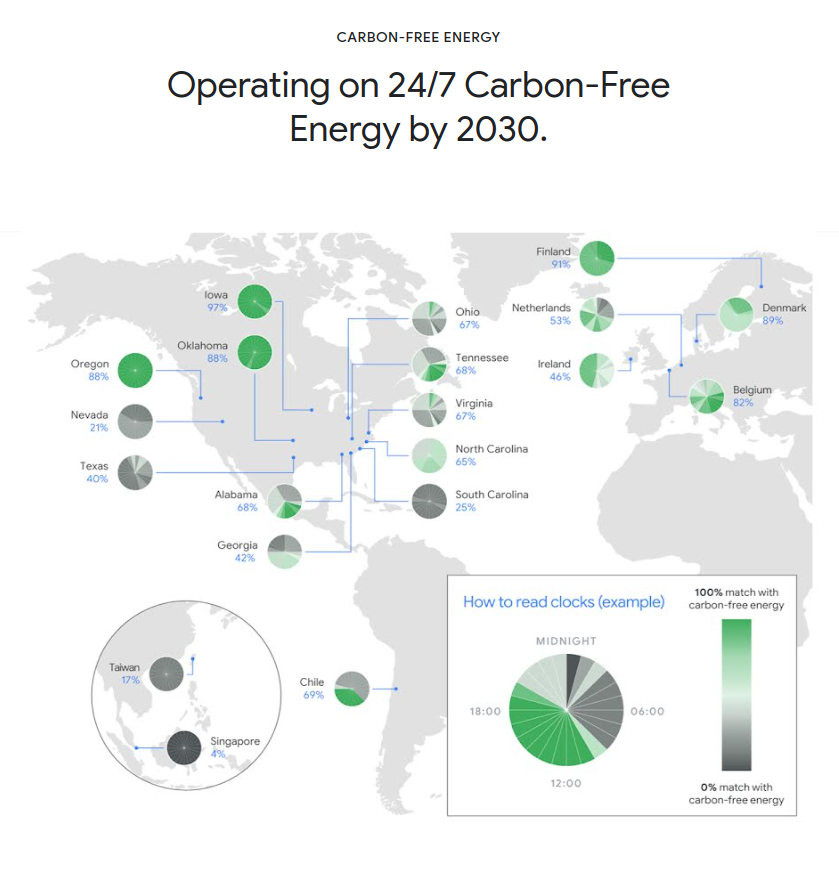
\includegraphics[width=6cm]{images/247-google-web.png}
    \vspace{.1cm}
  \end{column}

  \source{\href{https://sustainability.google/progress/energy/}{Image: sustainability.google/progress/energy/}}
  \end{columns}

  }
\end{frame}


\begin{frame}{Introduction}

  {\footnotesize
  \begin{itemize}
  \item In October 2022, we published a study on the \hrefc{https://zenodo.org/record/7180097}{"System-level impacts of 24/7 carbon-free electricity procurement in Europe"} \\
  \faGithub~\hrefc{https://github.com/PyPSA/247-cfe/releases/tag/v0.1}{Code behind the study}. 
  
  \item In the study, we investigated the \alert{means and costs} of pursuing different clean electricity procurement strategies for companies in a selection of European countries. We also explored how the 24/7~CFE commitments \alert{affect the European electricity system} as a whole. 
  
  \item The study concluded with the following take-aways: \\ 
  (i) 24/7~CFE commitments lead to lower emissions for both the
  participants and the system;\\ 
  (ii) 24/7~CFE also reduces the needs for flexibility in the rest of the system; \\ 
  (iii) Reaching CFE for 90-95\% of the time can be done with only a small cost premium. Reaching 100\% CFE target is possible but costly with existing renewable and storage technologies, with costs increasing rapidly above 95\%. 100\% CFE target could have a much smaller cost premium if long duration storage or clean firm generation technologies are available. \\ 
  (iv) 24/7 CFE procurement stimulates innovation and learning, and creates an early market for the advanced technologies.

  \item  These European study results align with the results in studies done by \hrefc{https://acee.princeton.edu/24-7/}{Princeton ZERO lab (2021)} for regions in the United States and by \hrefc{https://www.iea.org/reports/advancing-decarbonisation-through-clean-electricity-procurement}{IEA (2022)} for regions in Asia and Indonesia.

  \end{itemize}
  }

\end{frame}
  


\begin{frame}{Motivations}

  {\footnotesize
  \begin{itemize}
  \item In the previous study, however, we focused on a large range of European companies from the commercial and industry (C\&I) sectors that join 24/7~CFE efforts in aggregate. The implicit assumption we made was that all 24/7~CFE participants have \alert{inflexible demand}.
  
  \item In reality, many participants of the 24/7~CFE movement have some degree of flexibility in their electricity consumption. This flexibility takes the form of various demand response mechanisms available for \hrefc{https://doi.org/10.1016/j.rser.2021.111963}{a wide range} of commercial and industry consumers.

  \item  A \hrefc{https://cerre.eu/publications/data-centres-and-the-energy-grid}{large potential for demand side flexibility} is available in the information and communications technology (ICT) sector. Big companies such as Amazon, Google, IBM, and Microsoft are centralizing data centers to achieve economies of scale and form a computing infrastructure that is managed collectively via network operation centers. Thus, data center operators have the ability to \alert{shift computing jobs and associated power loads} in time (via scheduling of flexible compute jobs) and in space (via migration of flexible compute jobs across locations). 
  \end{itemize}

  }

\end{frame}
  

\begin{frame}{Why is this important? 1/2}

  {\footnotesize

  \begin{columns}[T]
    \begin{column}{9cm}
      \begin{itemize}
        \item   
        Demand for computing resources and data center power is rapidly growing, now representing nearly \hrefc{https://doi.org/10.1126/science.aba3758}{1\% of final electricity demand} worldwide. 
        Data centres and data transmission networks are responsible for \hrefc{https://www.iea.org/reports/data-centres-and-data-transmission-networks}{0.9\% of energy-related GHG emissions} (around 300~Mt \co-eq in 2020).
      
        \item Despite rapidly growing demand for digital services, the growth of associated emissions was modest due to energy efficiency improvements, decarbonisation of electricity grids and renewable energy purchases by ICT companies above and beyond the policy obligations. Based on \hrefc{https://www.iea.org/reports/data-centres-and-data-transmission-networks}{IEA (2022)} estimates, Amazon, Microsoft, Meta and Google have become the four largest purchasers of corporate renewable energy, having contracted over 38~GW to date with power purchase agreements (PPAs).
      
        \item Moreover, some of the ICT companies have become the front runners of the 24/7~CFE movement. Google has committed to the goal of \hrefc{https://www.gstatic.com/gumdrop/sustainability/247-carbon-free-energy.pdf}{24/7 Carbon-Free Energy by 2030}. Similarly, Microsoft has announced own \hrefc{https://blogs.microsoft.com/blog/2021/07/14/made-to-measure-sustainability-commitment-progress-and-updates/}{100/100/0 by 2030} commitment.

      \end{itemize}
      \end{column}
  
      \begin{column}{6cm}
      \centering
      \vspace{.3cm}
      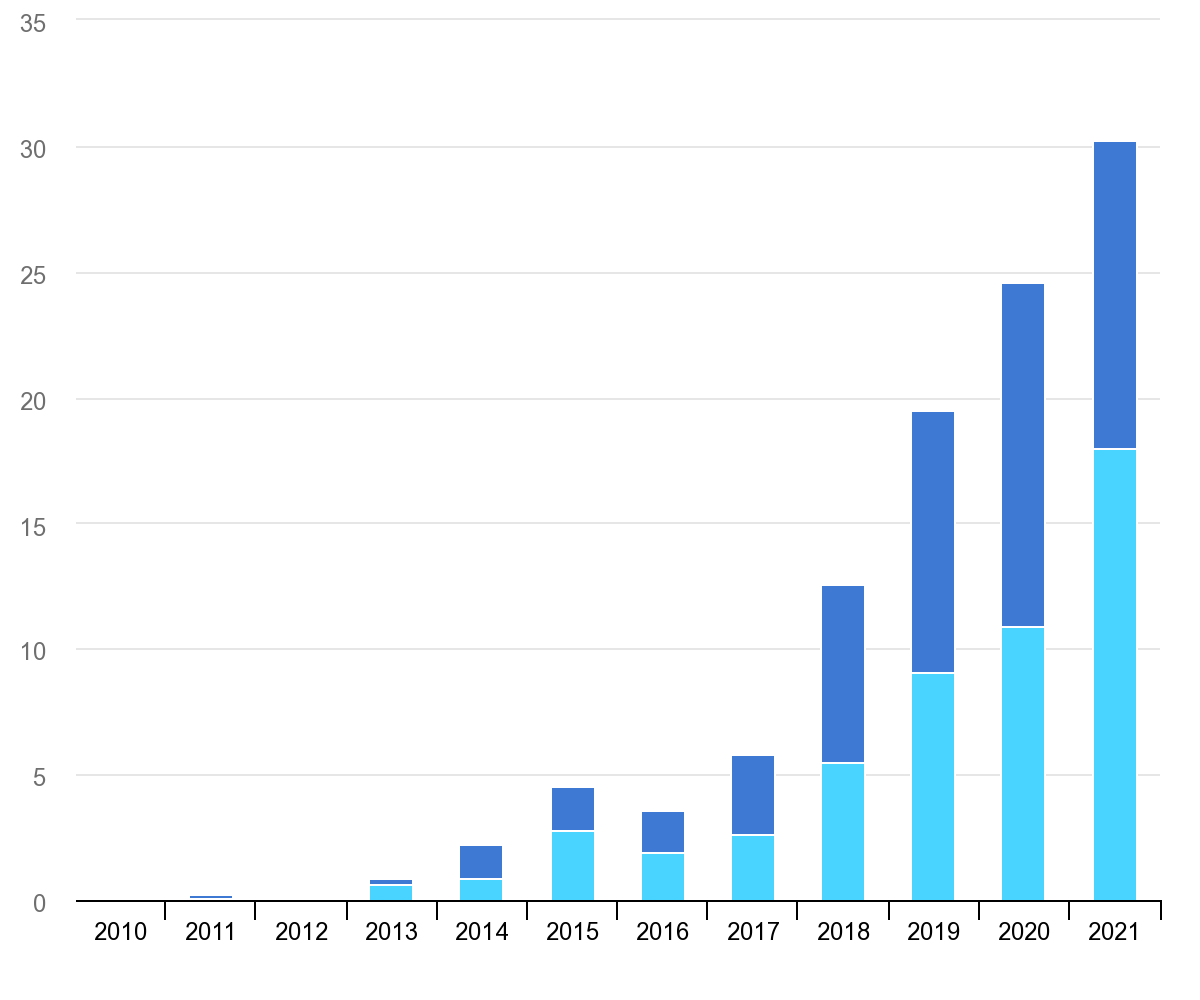
\includegraphics[width=6cm]{images/iea-PPAbysector-2010-2021.png}
      {\scriptsize
      Renewable energy capacity procured with power purchase agreements globally~[GW]. \\
      ICT sector (dark blue), all other sectors (light blue)}
    \end{column}
  
    \source{\href{https://www.iea.org/reports/data-centres-and-data-transmission-networks}{Image: IEA 2022}}
    \end{columns}

  }
\end{frame}


\begin{frame}{Why is this important? 2/2}

  {\footnotesize

  \begin{columns}[T]

    \begin{column}{6cm}
      \centering
      \vspace{.5cm}
      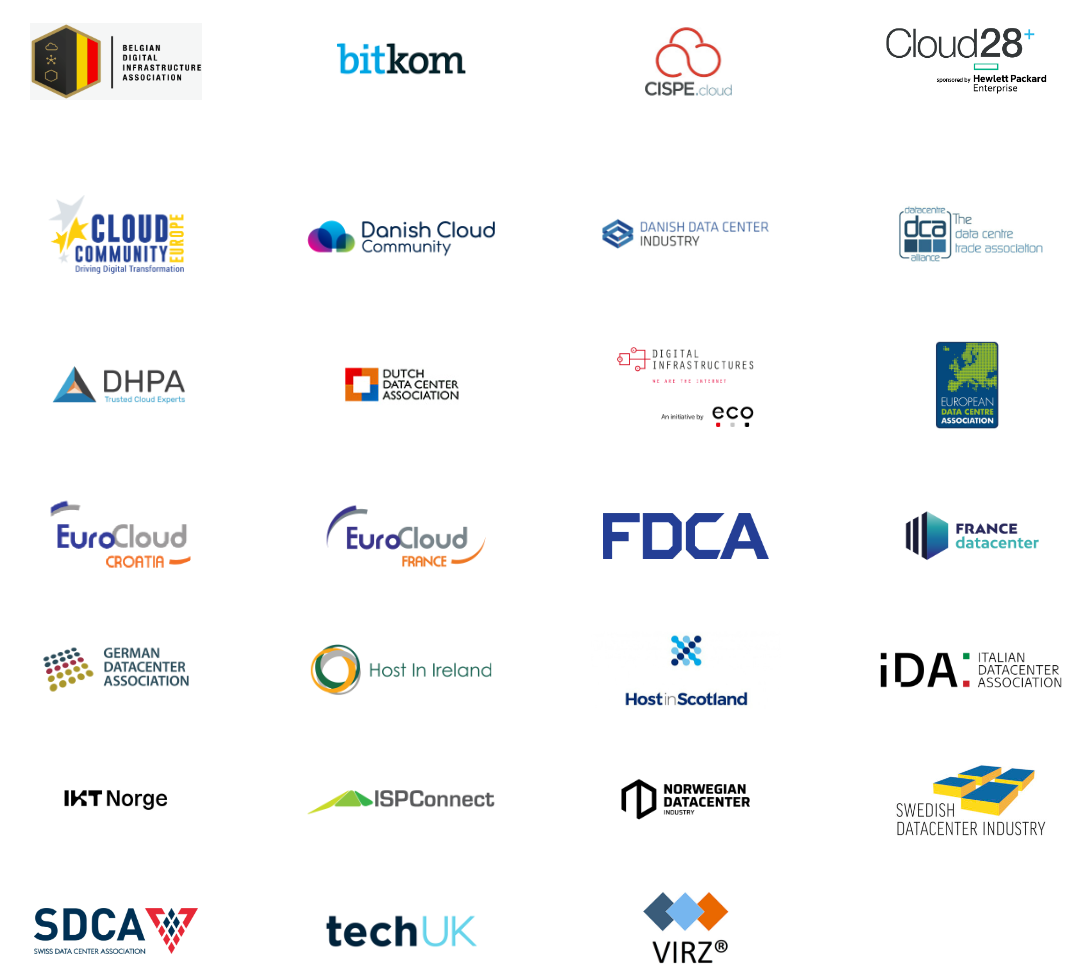
\includegraphics[width=6cm]{images/climateneutraldatacentre.png}
      {\scriptsize
      Data centre operators (Pact Associations) that signed \\ 
      the Climate Neutral Data Centre Pact}
    \end{column}

    \begin{column}{9cm}

      \begin{itemize}
        \item  The initiatives to measure and reduce the environmental impacts of digital infrastructure is spanning far beyond big companies like Google and  Microsoft.
        
        \item In 2021, over 100 data data centre operators and industry associations in Europe signed \hrefc{https://www.climateneutraldatacentre.net/}{the Climate Neutral Data Centre Pact} aiming to make data centres climate neutral by 2030. The pledged targets include measures to increase power usage effectiveness and carbon-free energy supply. The CFE target is declared to be \enquote{[..] 75\% of renewable energy or hourly carbon-free energy by December 31, 2025 and 100\% by December 31, 2030.} 

        \item Considering (i) a constant growth of global internet traffic, (ii) a large electricity consumption of data centers distributed in power grids worldwide, and (iii) the need to rapidly decarbonise electricity systems across the globe, it is \alert{important to understand the possible efficiency benefits that space-time load shifting flexibility can provide for the 24/7 carbon-free energy paradigm}. 

      \end{itemize}
      \end{column}
  

    \source{\href{Image: https://www.climateneutraldatacentre.net/signatories/}{Image: climateneutraldatacentre.net/signatories/}}
    \end{columns}

  }
\end{frame}



\begin{frame}{A growing body of research}

  {\footnotesize
  \begin{itemize}

  \item The unique characteristics of data centers as electricity consumers and the active interest of ICT sector companies in sustainable energy drive a growing interest in the research community. Among many other, \hrefc{https://doi.org/10.1016/j.simpat.2015.01.005}{Wang et al. (2015)}, \hrefc{https://doi.org/10.1016/j.comcom.2014.03.004}{Toosi et al. (2017)},
  \hrefc{https://doi.org/10.1016/j.future.2018.03.049}{Grange et al. (2018)},
  \hrefc{https://doi.org/10.1016/j.comcom.2014.03.004}{Velasco et al. (2018)}, and
  \hrefc{https://doi.org/10.1016/j.jcss.2020.11.004}{He \& Shen (2021)} investigated selected aspects of spatial or temporal demand management strategies in the context of supplying data centers power demand with intermittent renewable energy supply. 
  
  \item \hrefc{https://doi.org/10.1016/j.apenergy.2022.119930}{Zhang \& Zavala (2022)} elaborated a mathematical problem that captures both spatial \& temporal load-shifting flexibility provided by data centers. The authors suggest market clearing formulation treats data centers as prosumers that simultaneously request load and provide a load-shifting flexibility service to the grid. The illustrated clearing formulation satisfies fundamental economic properties of the competitive markets, such as revenue adequacy and cost recovery.

  \item The Google research team published a paper on \hrefc{https://doi.org/10.1109/TPWRS.2022.3173250}{Carbon-Aware Computing for Datacenters} \href{https://doi.org/10.1109/TPWRS.2022.3173250}{(Radovanović~et~al.~(2023})). The paper introduced methodology and principles behind a carbon-intelligent compute management system, which minimizes electricity-based carbon footprint and power infrastructure costs by shifting temporally flexible workloads for all datacenter clusters across Google's fleet.

  \end{itemize}
  }

\end{frame}


\begin{frame}{Focus of the study}

  {\footnotesize
  \begin{itemize}
    \item In this study, we explore the potential benefits for 24/7 carbon-free energy buyers and rest of energy system associated with demand flexibility. We aim to answer the following questions: \\

    \vspace{0.1cm}
    -- How can demand flexibility reduce the \alert{resources} and \alert{costs} for 24/7~CFE matching?\\ 
    -- How can demand flexibility promote \alert{economic efficiency}?\\
    -- What are the \alert{individual effects} of spatial and temporal demand flexibility, as well what are the synergies from their co-optimization? \\
    -- How would advanced technologies, such as long duration storage, affect \alert{the value of demand flexibility}?

    \item For this purpose, we elaborate the mathematical model developed in the previous study, by including spatial and temporal demand flexibility provided by electricity consumers following 24/7~CFE goal. Thus, a flexible 24/7 participant could benefit from \alert{co-optimising} utilisation of available demand flexibility (across space and/or time) and procurement strategies to match every kWh of electiricty consumption with carbon-free energy around-the-clock \alert{more efficiently}.
    
    \item The modelling exercise in this study is focused on \textit{data centers}, i.e., facilities used to house networked computer servers that store, process and distribute large amounts of data. Nevertheless, the findings of this study are likely to be of interest to a wide range of companies and organisations with flexible demand and an interest in 24/7 carbon-free energy procurement, as well as to energy industry experts and stakeholders with an empirical interest in the European energy system.

  \end{itemize}

  }
\end{frame}



%----------------------------------------
%----------------------------------------
\section{Study design}


\begin{frame}
  \frametitle{A quick overview}

{\footnotesize
  \begin{itemize}
    
    \item This study is done in a spirit of open and reproducible research. The whole scientific workflow from the publicly available raw input data to optimized electricity system, visualizations and compilation of this study is available at \hrefc{https://github.com/PyPSA/247-cfe}{github.com/PyPSA/247-cfe}. 
    
    \item In this study, we build upon the mathematical model of 24/7~CFE procurement developed in the former work of authors: \hrefc{https://zenodo.org/record/7180097}{System-level impacts of 24/7 carbon-free electricity procurement in Europe} (October 2022)
    
    \item We encode a set of new equations and routines, which allow for modelling \alert{spatial} (computing jobs migration) and \alert{temporal} (computing jobs scheduling) load flexibility provided by data centers.

    \item We place data centers (i.e., electricity consumers committed to 24/7~CFE goals) in a selection of European countries: Ireland, Denmark, Germany, Finland, and Portugal. These countries have different weather patterns, renewable potentials, national energy and climate policies, legacy fleets of generation capacities, degree of interconnectons, etc. Apart form that, we consider several scenarios for CFE procurement targets, degrees of data center flexibility, and technologies available for 24/7 consumers. These differences help to \alert{understand and generalize} the interplay of demand flexibility and 24/7~CFE procurement.

  \end{itemize}
}
\end{frame}


\begin{frame}{Study design: European power system}
  
  {\footnotesize
  \begin{columns}[T]

  \begin{column}{7cm}
  \centering

  \vspace{0.6cm}
  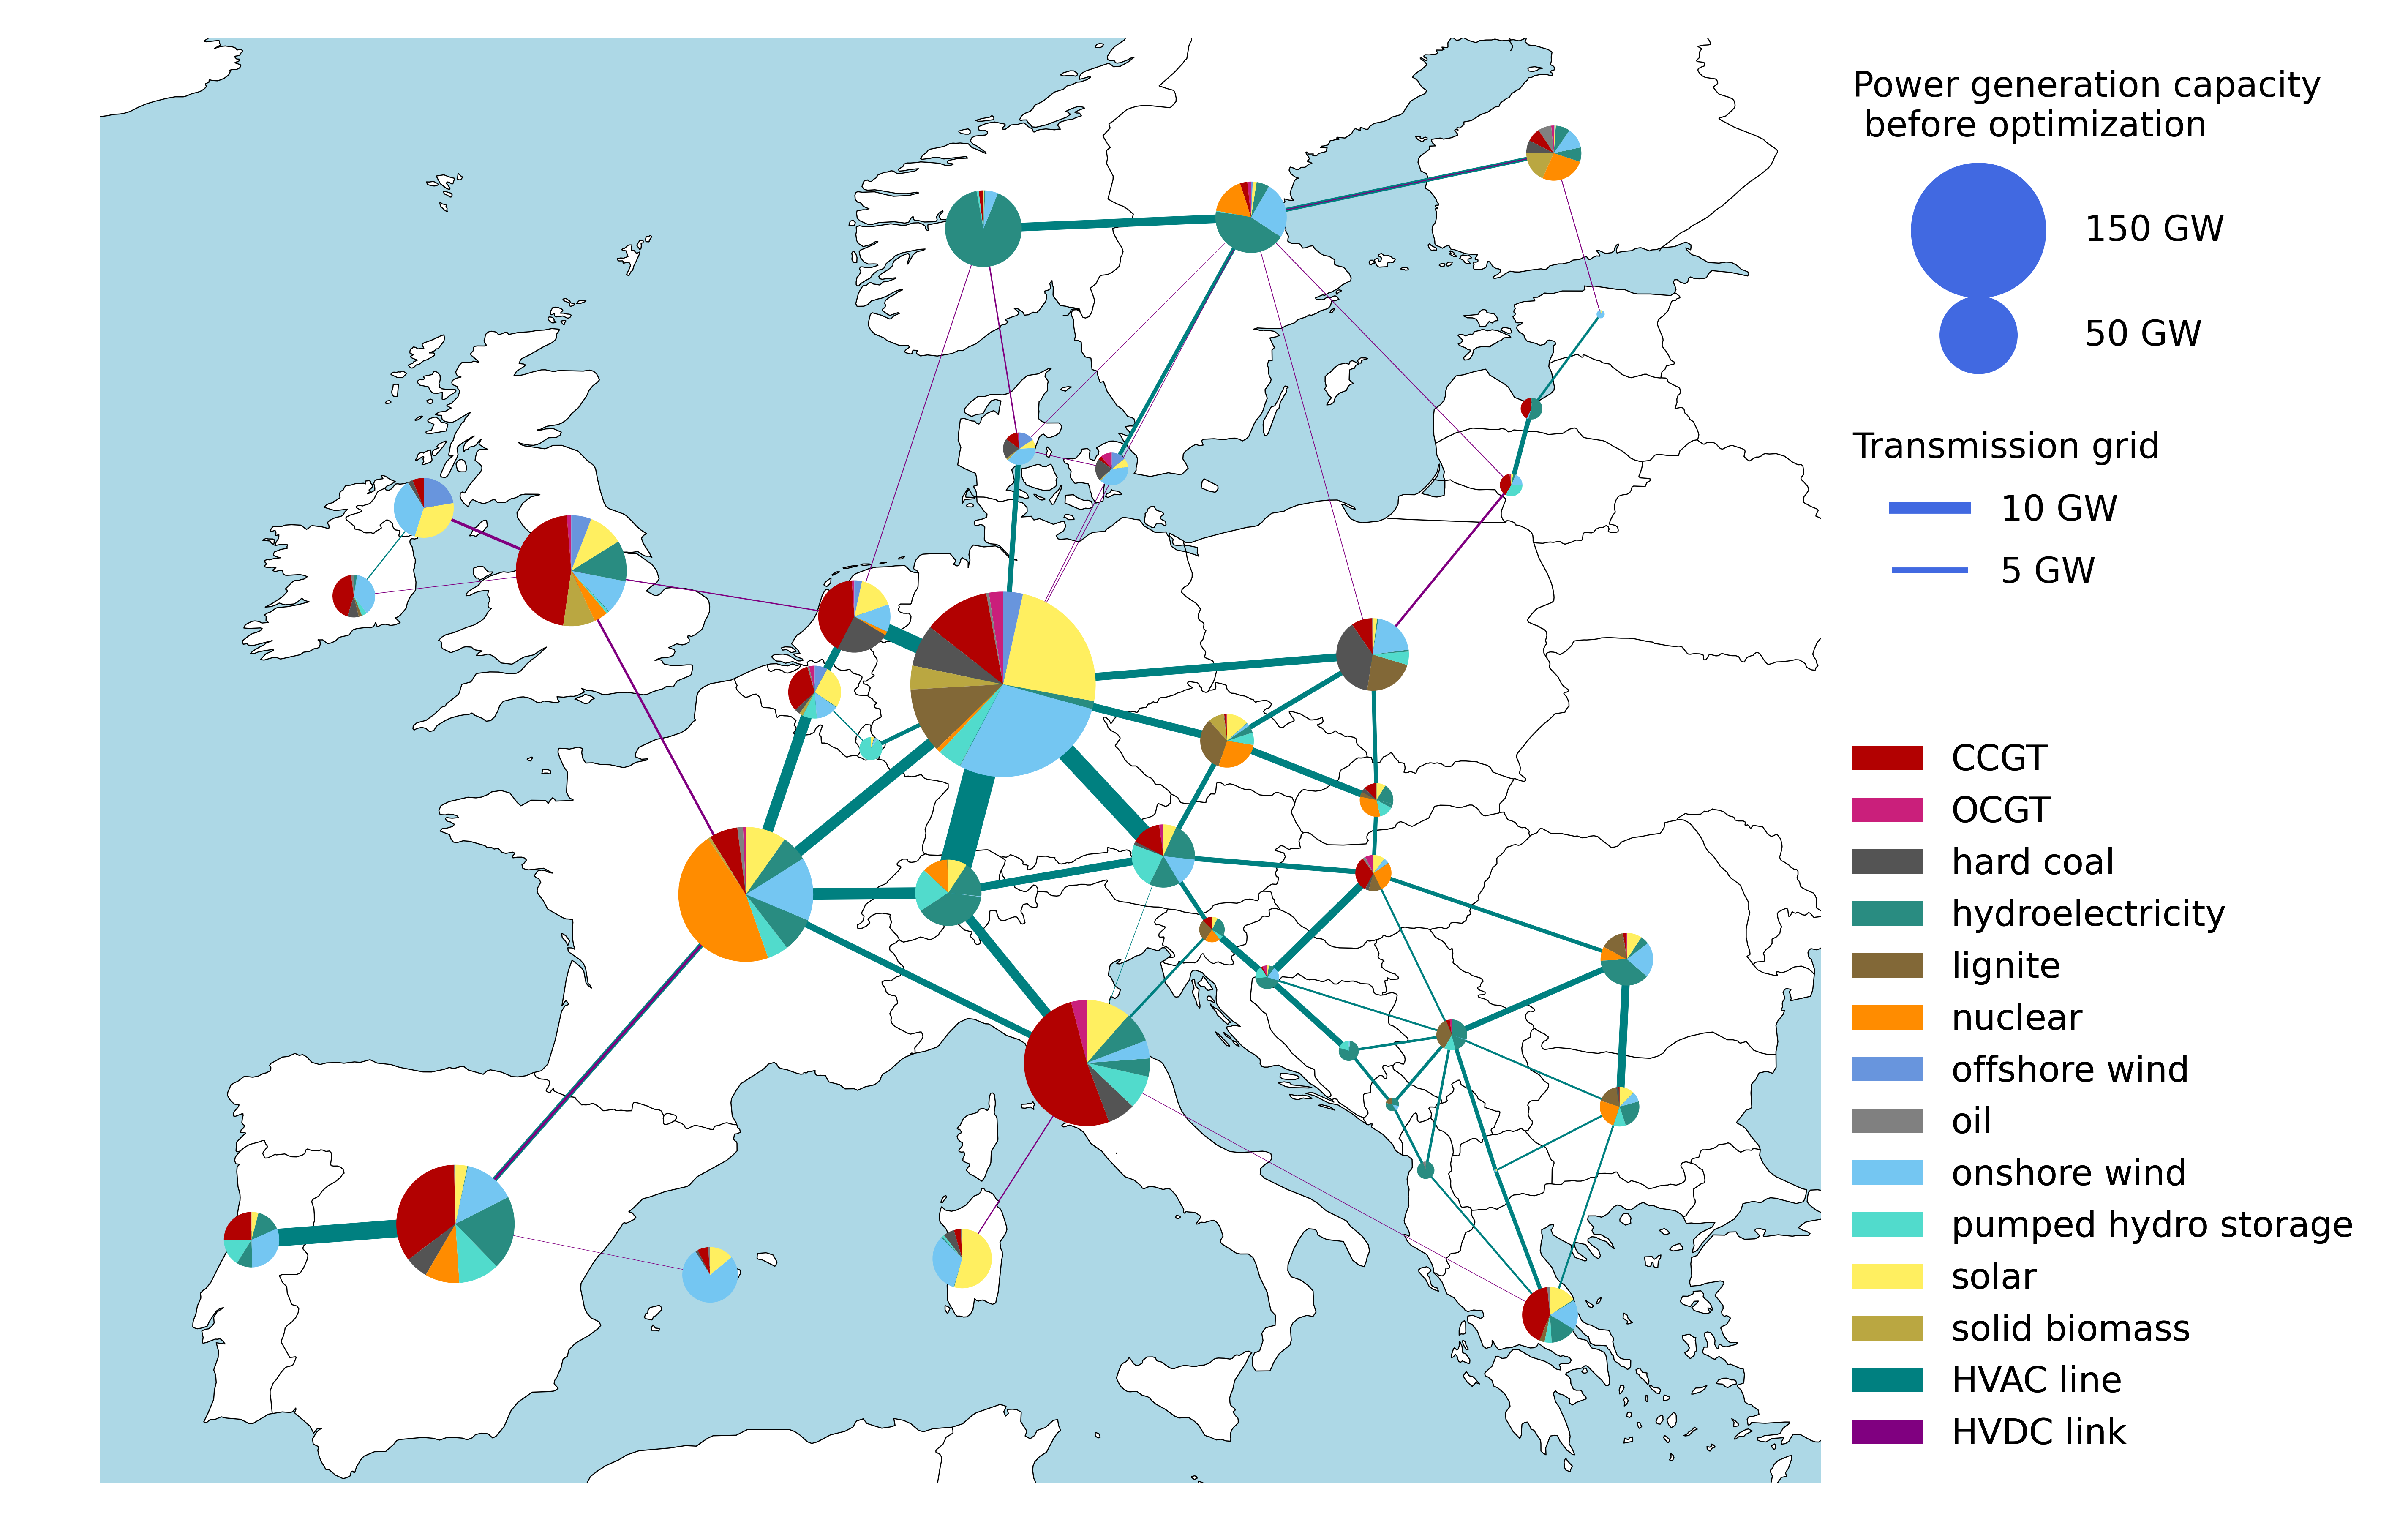
\includegraphics[width=7.7cm]{images/map-fleet.pdf}
  {\scriptsize European electricity system clustered to 37 zones \\ 
  NB power generation capacity fleet before optimization}
  \end{column}

  \begin{column}{8cm}
  \begin{itemize}
  \vspace{-0.2cm}
  \item In each scenario, we model the full European power system (\hrefc{https://www.entsoe.eu/data/map/}{ENTSO-E area}) 
  clustered to \alert{37~zones}. Each zone represents an individual country. Some countries
  that straddle different synchronous areas are split to individual bidding zones, 
  such as DK1 (West) and DK2 (East).

  \item The model \alert{co-optimizes} investment and dispatch decisions of generation \& storage assets to meet electricity demand of data centers (flexible 24/7~CFE consumers), as well as investment and dispatch decisions of assets in the rest of the European electricity system to meet the demand of other consumers. 
  
  \item The modelling is done for \alert{2025}. Input data such as technology cost assumptions,
  national renewable policies, decommissioning of legacy power plant fleet, and system-wide assumptions (e.g., price for EU ETS) are parametrised accordingly.

  \item All model runs are done with \alert{hourly resolution}, i.e., no time sampling.
  
  \end{itemize}

  \end{column}
  \end{columns}
  }

\end{frame}



\begin{frame}{Study design: data centers}
  
  {\footnotesize
  \begin{columns}[T]

  \begin{column}{7cm}
  \centering
  \vspace{0.5cm}
  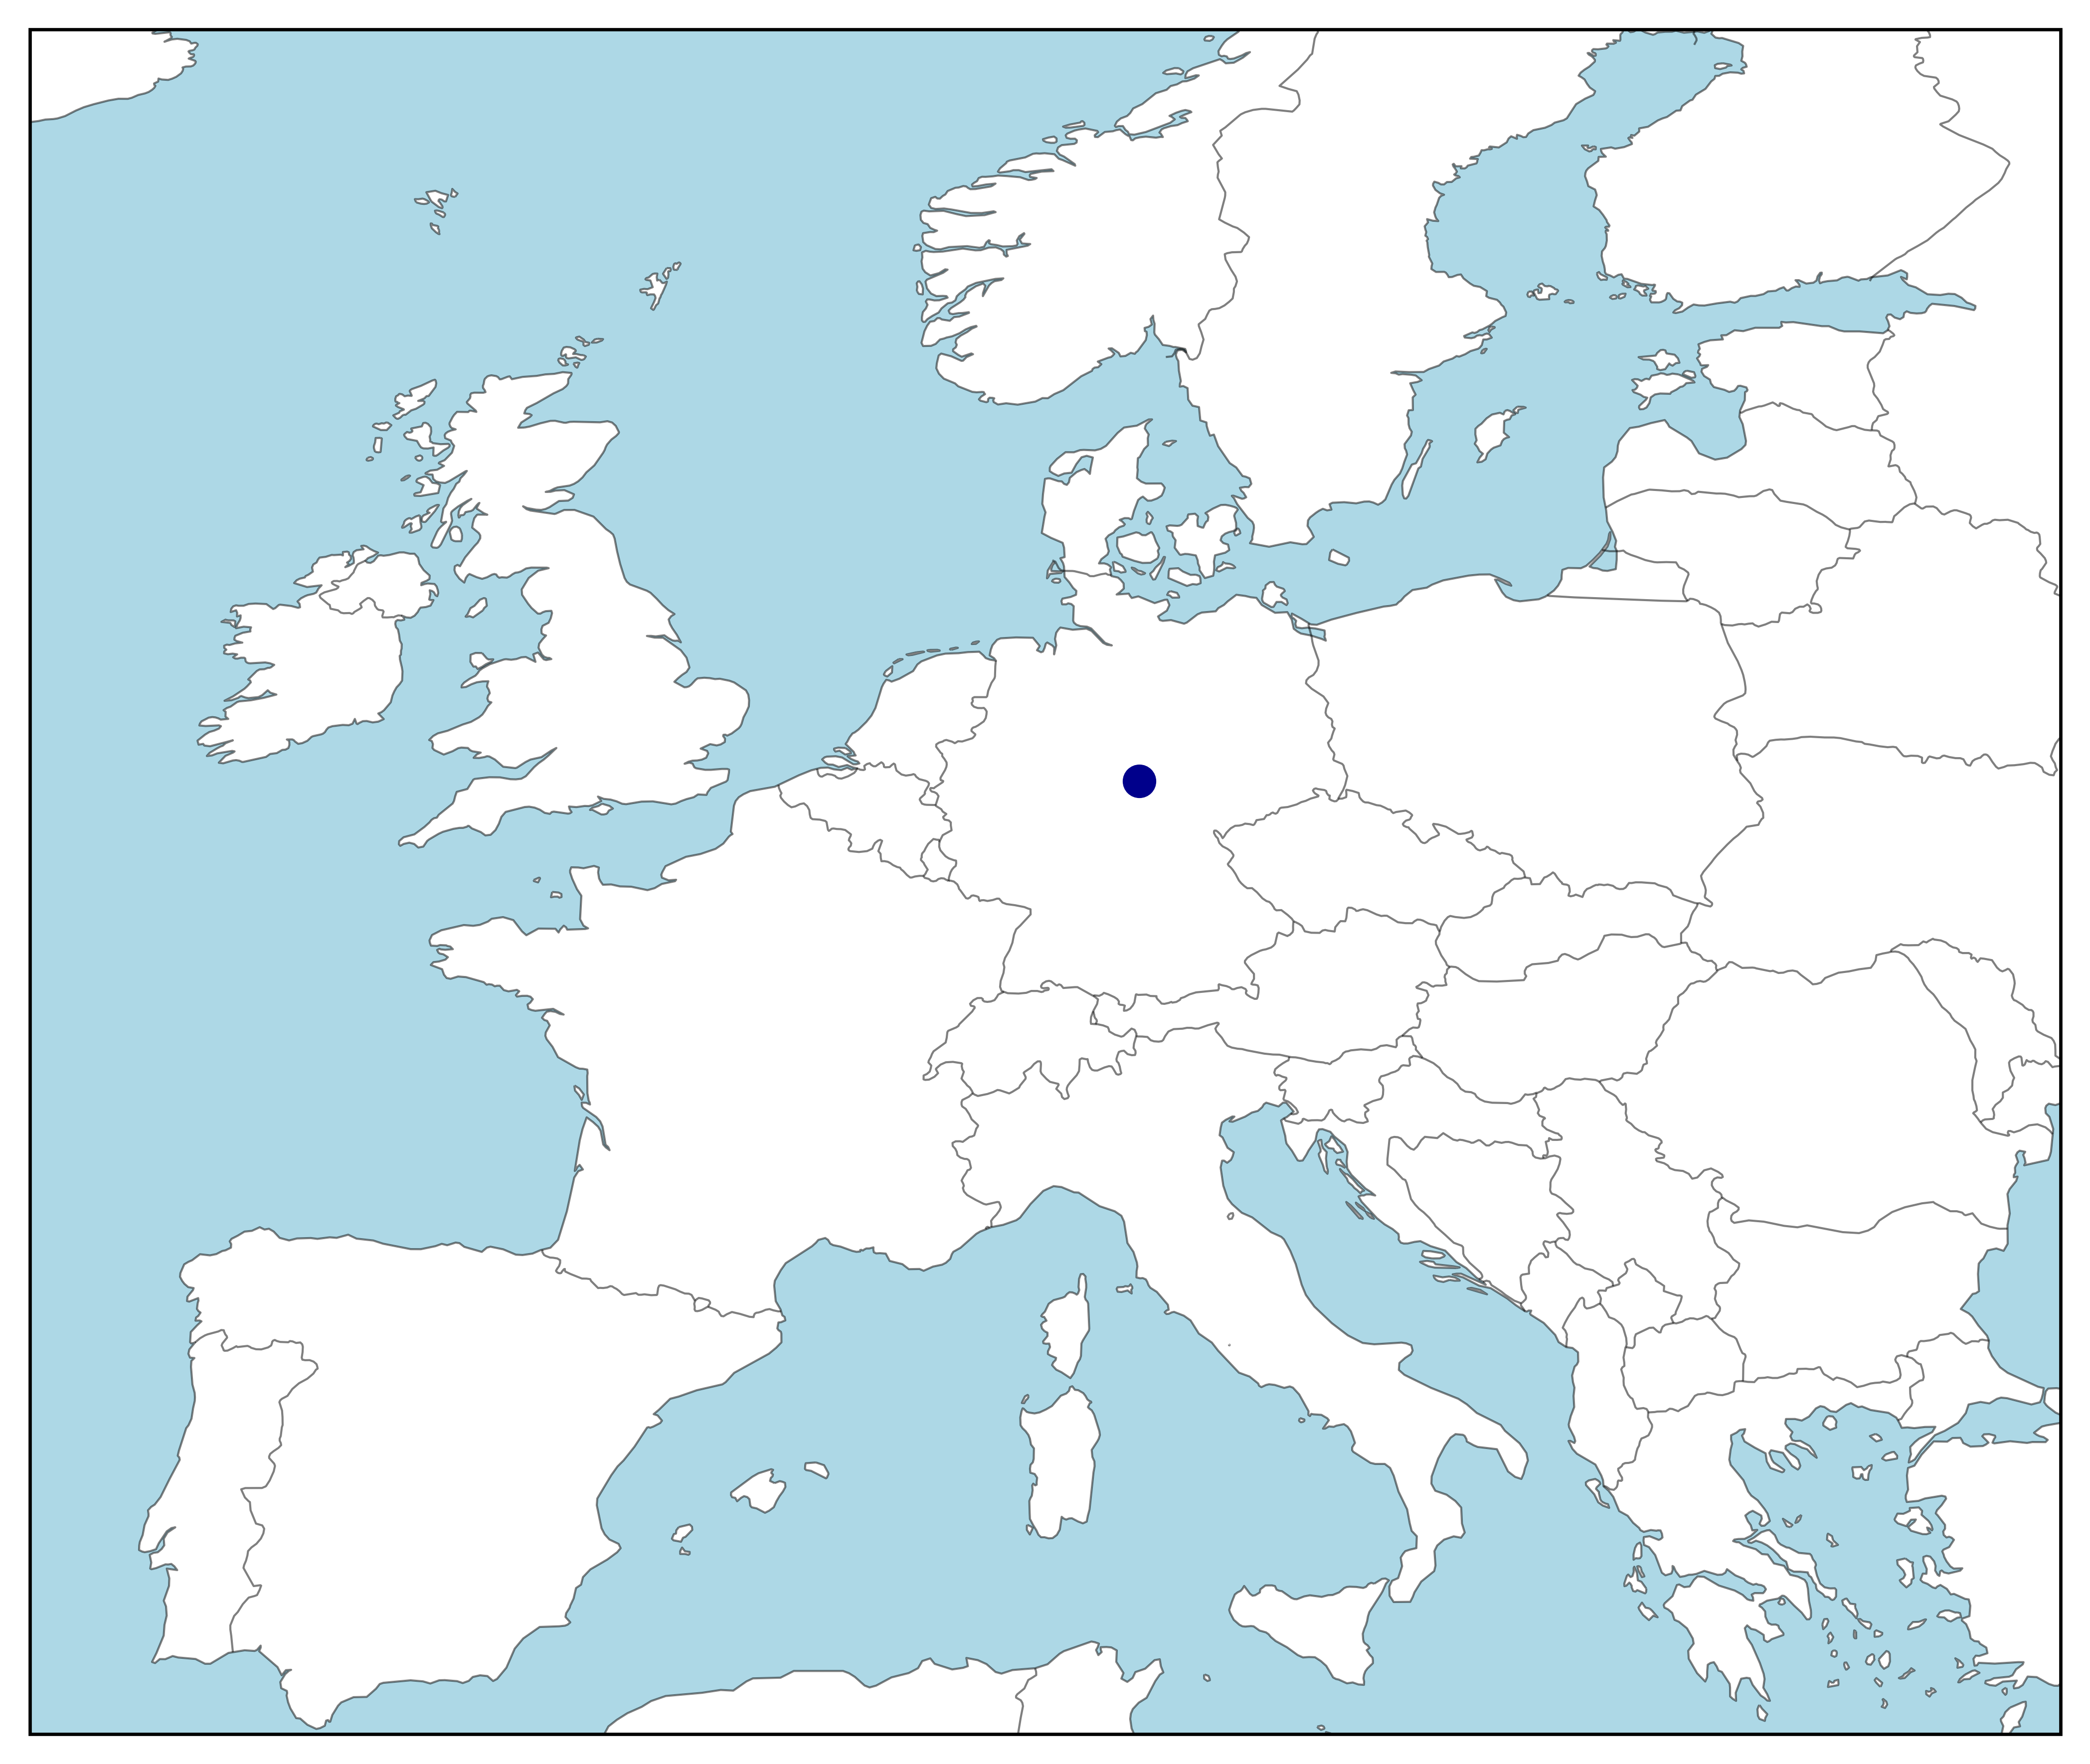
\includegraphics[width=7cm]{images/map-DCs.pdf}
  {\scriptsize Five data centers interconnected by virtual links, \\ 
  forming a complete graph}
  \end{column}

  \begin{column}{8cm}
  \begin{itemize}
    \item We consider \alert{five data centers} that are located in Ireland, Denmark (West/DK1), Germany, Finland, and Portugal. These locations (i) include zones where data centers have an important share in national electricity demand [\hrefc{https://www.statista.com/statistics/878621/european-data-centers-by-country/}{1},\hrefc{https://backend.orbit.dtu.dk/ws/portalfiles/portal/236202284/The_role_of_data_centres_in_the_future_DES_clean_version.pdf}{2},\hrefc{https://www.cso.ie/en/releasesandpublications/ep/p-dcmec/datacentresmeteredelectricityconsumption2021/keyfindings/}{3}], and (ii) include zones that have electricity systems with unique characteristics, such as local generation mix, renewable potentials, national energy and climate policies, degree of interconnections, etc. 
    \item Data centers have a nominal load of \alert{100~MW} (baseload profile). The data center operator aims to achieve a given 24/7~CFE matching score \alert{at all locations}. 
    \item Data centers are interconnected by \enquote{virtual links} (non-physical pathways between data centers) forming a \alert{complete graph}, i.e., every pair is connected by a unique virtual link.
    \item Data centers have the \alert{same share of flexible workloads}. 
  \end{itemize}

  \end{column}
  \end{columns}
  }

\end{frame}



\begin{frame}{Study design: data center load flexibility}

  {\footnotesize
    \begin{columns}[T]
  
    \begin{column}{6cm}
    \centering
    \vspace{0.2cm}
    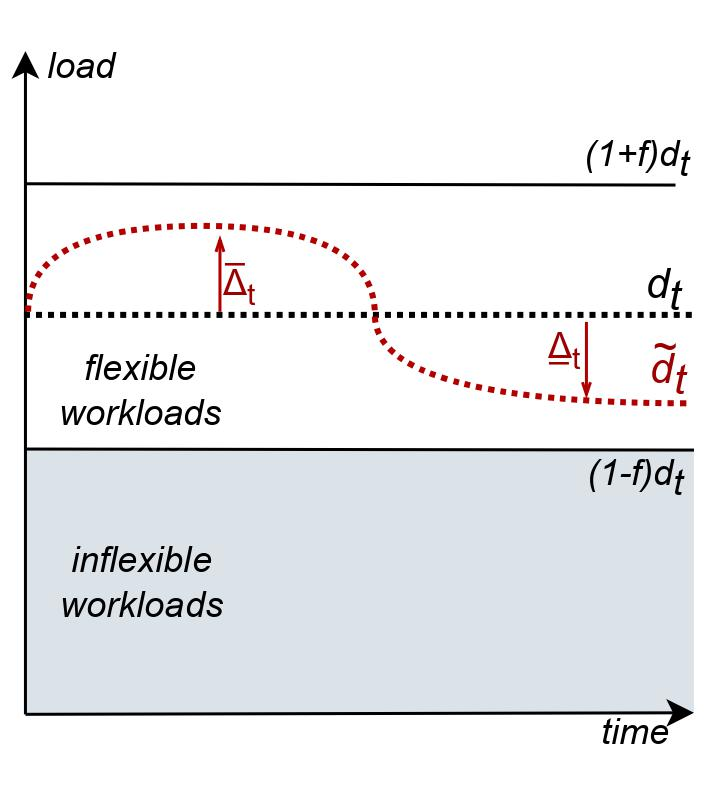
\includegraphics[width=6cm]{images/drawio_flexrange_d.pdf}
    \end{column}
  
    \begin{column}{9cm}
    \begin{itemize}
    \vspace{-0.1cm}
    \item The premise of data center flexibility is that a known number of computing jobs, and associated power usage is \enquote{flexible}, i.e., electricity loads can potentially be shifted in space (across datacenter locations), or to other times (by delaying jobs' execution).\footnote{{\scriptsize A change in cluster-level CPU usage can be accurately mapped into a change in its power usage, see \href{https://arxiv.org/abs/2106.11750}{Radovanovic et al. (2021)}}}
  
    \item Thus, the \alert{dispatched load $\widetilde{d}_t$} of a data center can deviate from the nominal requested load $d_t$. The dispatched load $\widetilde{d}_t$ is constrained by the data center capacity (an upper limit) and the inflexible loads (a lower limit). The range of possible deviations of the dispatched and nominal loads is assumed to lie within $f$~[\%] of the nominal load, such as:
    \begin{subequations}
      \begin{align}
        [1-f] \cdot d_t \le  \widetilde{d}_t  \le [1+f] \cdot d_t \quad \forall t \in T  
        \label{eqn:range} \\
        \widetilde{d}_t = d_t + (\overline{\Delta}_t - \underline{\Delta}_t) \quad \forall t \in T  
        \label{eqn:widetilde}
      \end{align}
    \end{subequations}
    \noindent where $\overline{\Delta}_t, \underline{\Delta}_t \in \mathbb{R}_{+}$ stand for positive/negative deviation of $\widetilde{d}_t$ and $d_t$ in hour $t$.
    \end{itemize}
  
    \end{column}
    \end{columns}
  }
  \end{frame}



\begin{frame}{Study design: space-time load shifting}

  {\footnotesize
  \begin{columns}[T]
  
  \hspace{-1.5cm}
  \begin{column}{10cm}
  \vspace{0.3cm}
  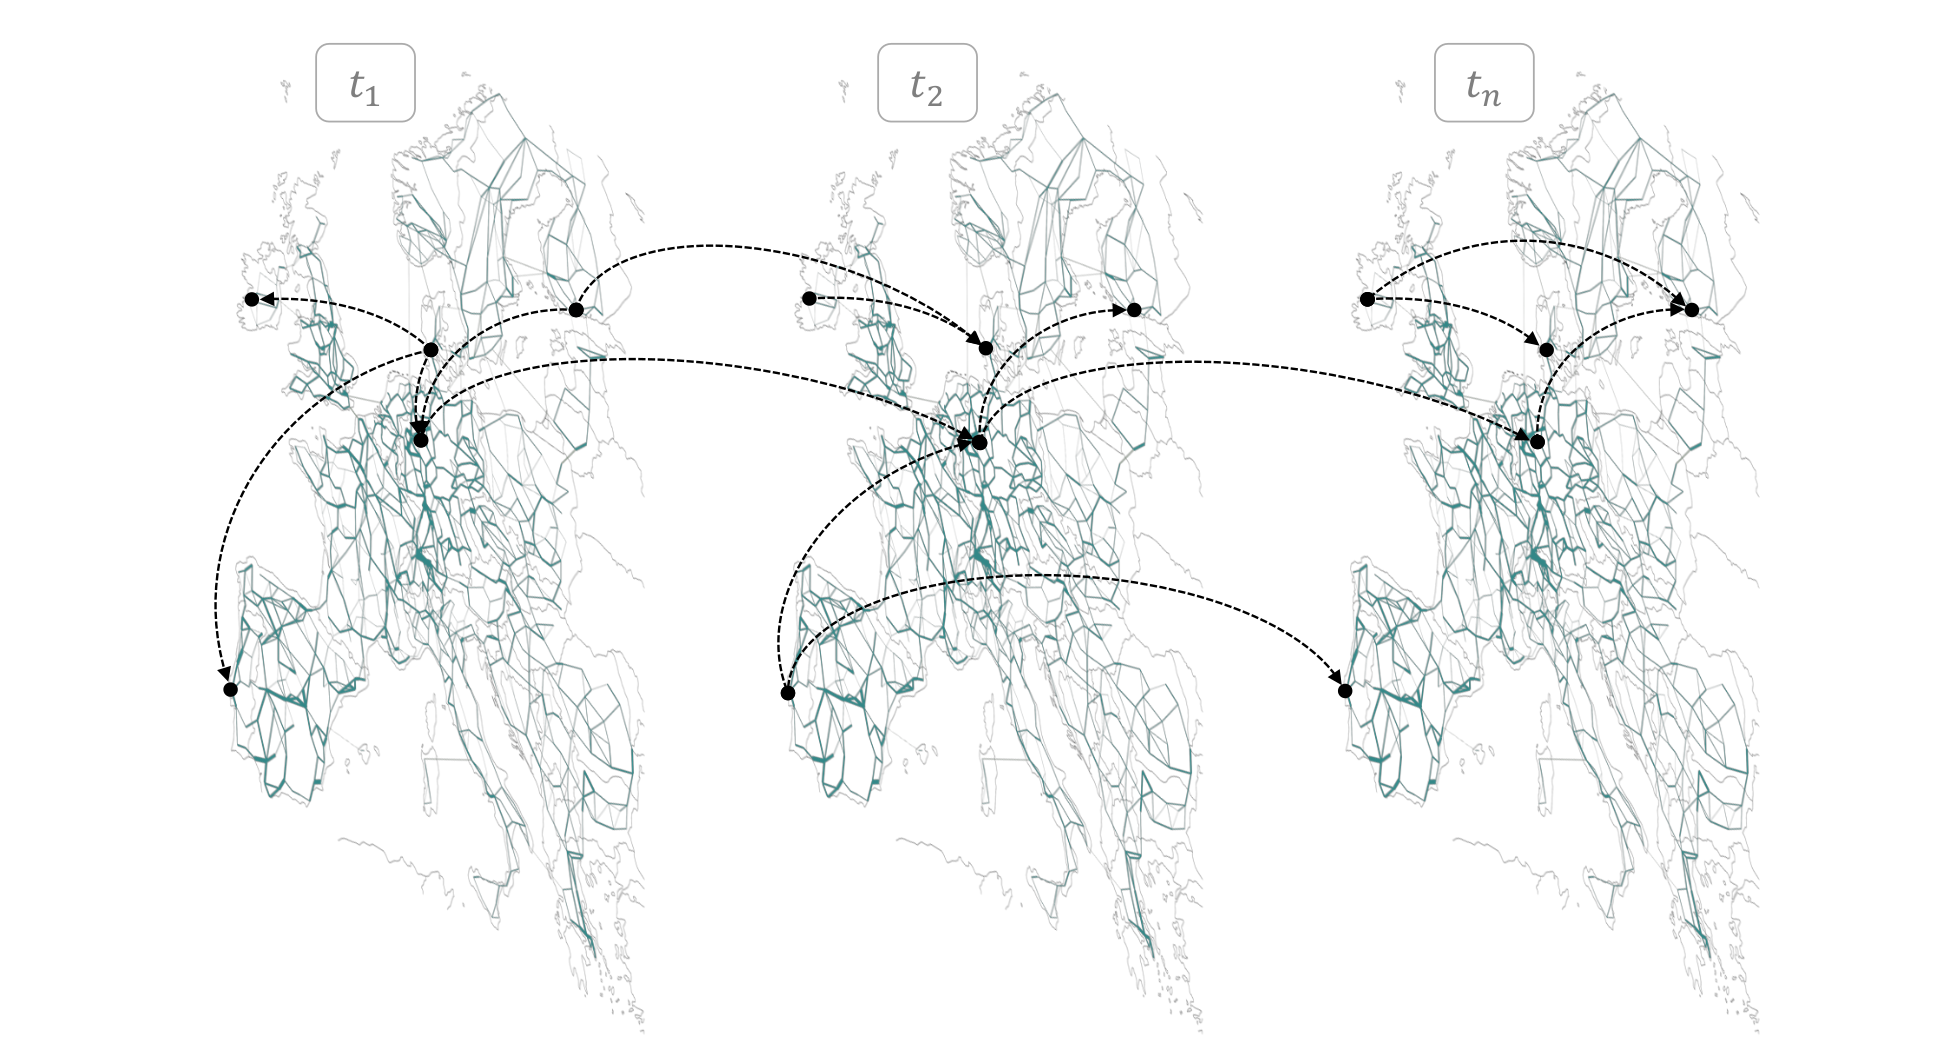
\includegraphics[width=11.5cm]{images/spatial-temporal-vlinks.png}
  \end{column}

  \begin{column}{6cm}
  \begin{itemize}
    \vspace{0.3cm}
    \item To capture spatial flexibility, we implement a spatial load management system that can shift load across data center locations via virtual links.
    \item To capture temporal flexibility, we implement a load scheduling system that can shift load of a data center over time.
    \item For the mathematics and detail on the optimization model, see \alert{\hyperlink{methodology}{Annex A: Methodology}}.
  \end{itemize}

  \end{column}
  \end{columns}
  }
\end{frame}


\begin{frame}{Study design: scenario space}

  {\footnotesize 
  \begin{itemize}

  \item We model various scenarios for data center demand flexibility, which include \\
  \vspace{0.1cm}
  Three modes of operation: \\
    -- Co-optimized \alert{spatial and temporal} load management \\
    -- Isolated \alert{spatial} load management (shifting flexible workloads across locations)\\ 
    -- Isolated \alert{temporal} load management (shifting flexible workloads in time) \\ 
  \vspace{0.1cm}
  and four scenarios for flexible workloads range: \alert{$f$ = \{0\%, 10\%, 20\%, 40\%\}}.

  \item Two scenarios for 24/7~CFE hourly matching targets:
  \alert{$CFE scores$ = \{98\% and 100\%\}}.
  
  \item Further, we assume two palettes of carbon-free technologies available for procurement for data center operators participating in 24/7-CFE: \\
  \vspace{0.1cm}
  -- \alert{Palette~1} includes technologies available on the European market now: onshore wind, utility scale solar PV, battery storage. \\
  -- \alert{Palette~2} includes all above plus Long Duration Energy Storage (LDES) in the form of a hydrogen storage system. 

  \item For interested parties, we publish an \faLink~\hrefc{tba}{online Annex} with a full pack of modelling results alongside this study. The materials include modelling results for all scenario combinations in a form of plots and summary csv files. 

  \end{itemize}
  }
\end{frame}



\begin{frame}{Study design: limitations}
  
  {\footnotesize 
  \begin{itemize}

  \item This study is done in a spirit of \alert{modelling for insight} rather than \alert{modelling for numbers}. The design of this study does not aim at quantifying the real-life benefits of demand side flexibility for data centers. It is rather a model experiment to explore \textit{why and how} flexibility of demand can be beneficial for achiving 24/7 carbon-free energy goals. The results we present can thus be viewed with a fair degree of caution, i.e., as a modelling-based insight rather than quantitative projection. 
  
  \item Quantifying the actual costs benefits for the ICT industry of utilising demand flexibility requires \alert{additional empirical research}. Further studies could usefully explore the costs of achieving a certain share of flexible workloads beared by data center operators, which are \alert{not considered} in this study. Including information on implicit flexibility costs would help to quantify the flexibility benefits with a greater degree of accuracy. Another empirical improvement could address technical aspects and properties of flexible workloads, such as physical constraints associated with quick ramping of power usage up/down, safety constraints, etc.
  
  \end{itemize}
  }
  \end{frame}


%---------------------------------------------
%---------------------------------------------
\section{Modelling results and analysis}



\begin{frame}{An overview}

  {\small 

  The results section is organized as follows:

  \begin{enumerate}

  \item \hyperlink{sec:procurement}{Procurement and 24/7 CFE costs as a function of load flexibility}.
  \item \hyperlink{sec:efficiency}{Economic efficiency of co-optimized space-time load shifts}.
  \item \hyperlink{isolated-hook}{Isolating values of spatial and temporal load shifting}.
  \item \hyperlink{ssec:time-series}{Insights from time-series data for optimized space-time load shifts}.
  \item \hyperlink{ssec:redistribution}{Economically efficient redistribution of data center average loads}.
  \item \hyperlink{ssec:remarks}{Further remarks}.

  \end{enumerate}
  }
  \end{frame}


%---------------------------------------- Portfolio and Costs
%----------------------------------------


\begin{frame}{Procurement as a function of load flexibility (100\% CFE)}
\label{sec:procurement}

  {\footnotesize
  \vspace{0.2cm}
  
  \begin{columns}[T]
  \begin{column}{9cm}
  \centering
  
  \includegraphics[width=9.2cm]{../results/1H-IEDKDEFIPT-allflex/plots/2025/EU/p1/cfe100/capacity.pdf}

  \end{column}

  \begin{column}{6cm}
  
  Let us first consider the following scenario:
  (i) 100\% CFE target, (ii) technology palette~1 (without LDES), and (iii)  co-optimized spatial \& temporal load flexibility.
  
  \vspace{0.1cm}
  A plot on the left shows the cost-optimal \alert{portfolio capacity} required to match demand with carbon-free electricity around-the-clock. Results are displayed per each location and share of flexible loads $f$.
  
  \vspace{0.1cm}
  As shown in the previous study, 100\% hourly matching with renewable generators and battery storage requires a large portfolio for inflexible demand case. The cost-optimal mix of solar PV, wind and battery storage depends on the local resources.

  \vspace{0.1cm}
  The required portfolio capacity \alert{is significantly reduced when load shifting becomes possible}. This effect takes place in all locations.
  \end{column}
  \end{columns}
  }
  \source{24/7 CFE 100\% -- palette~1 tech -- spatial \& temporal shifts}
\end{frame}


\begin{frame}{24/7~CFE costs as a function of load flexibility (100\% CFE)}

  {\footnotesize
  \vspace{0.2cm}
  
  \begin{columns}[T]
  \begin{column}{9cm}
  \centering
  \includegraphics[width=9.2cm]{../results/1H-IEDKDEFIPT-allflex/plots/2025/EU/p1/cfe100/ci_costandrev.pdf}
  \end{column}

  \begin{column}{6cm}
  The \alert{cost breakdown} on the left shows the average costs (per MWh of consumption) of meeting demand with the 24/7~CFE policy netted by revenue selling to the regional grid. (NB for the 100\% CFE target, 24/7 consumers have nearly no grid imports in the consumption mix.) With inflexible demand, only selected regions benefit from good resources for solar (PT) or wind (DK) and achieve hourly CFE matching with lower costs. Overall, the 100\%~CFE hourly matching target remains costly with palette~1 technologies.

  \vspace{0.1cm}
  \alert{Load shifting reduces the costs for 24/7 procurement in all locations}, and especially in locations where hourly matching with CFE is expensive (IE, DE). Flexibility evens out the average costs across locations, making 24/7~CFE more affordable in resource-constrained places.

  \end{column}
  \end{columns}
  }
  \source{24/7 CFE 100\% -- palette~1 tech -- spatial \& temporal shifts}
\end{frame}
  


\begin{frame}{Procurement as a function of load flexibility (98\% CFE)}
  \label{cfe98portfolio}

  {\footnotesize
  \vspace{0.2cm}
  
  \begin{columns}[T]

  \begin{column}{6cm}
  If we now turn to a scenario with \alert{lower CFE target of 98~\%} (keeping technology palette~1 and both spatial \& temporal load flexibility enabled), we see that this procurement policy can be met by procuring much less onshore wind and solar capacity.
  
  \vspace{0.1cm}
  This observation is in line with the previous study, which showed that the last 2\% of hourly CFE matching nearly doubles the required resources and costs (without LDES or clean firm generation).

  \vspace{0.1cm}
  With a CFE target of 98\%, the total procured capacity still reduces in all locations with increasing potential for demand flexibility, i.e., increasing share of flexible workloads. The effects include (i) a reduction of battery storage, (ii) a small reduction of overall renewable capacity, and (iii) a swap of solar capacity with wind due to higher capacity factor of the latter. 
  
  \end{column}

  \begin{column}{9cm}
    \centering
    \includegraphics[width=9.2cm]{../results/1H-IEDKDEFIPT-allflex/plots/2025/EU/p1/cfe98/capacity.pdf}
  \end{column}
  \end{columns}
  }
  \source{24/7 CFE 98\% -- palette~1 tech -- spatial \& temporal shifts}
  \end{frame}


\begin{frame}{24/7~CFE costs as a function of load flexibility (98\% CFE)}
  \label{cfe98cost}

  {\footnotesize
  \vspace{0.2cm}
  
  \begin{columns}[T]

  \begin{column}{6cm}
  There are two distinct observations in the breakdown of costs for meeting the CFE 98\% policy: (i) the cost component associated with imports of electricity from the regional grid enters the mix of options to meet the CFE policy; (ii) as mentioned above, the net average cost of CFE procurement is much lower than for CFE~100\%.

  \vspace{0.1cm}
  Shifting of load across space and time \alert{enables access to clean electricity} at times of day when certain locations have high renewable penetration and \alert{creates more options to match demand with CFE} for times and locations where renewable potential is scarce (for details, we provide a time-series analysis below). 

  \vspace{0.1cm}
  As a result, CFE 98\% policy is more affordable in all locations with increasing demand flexibility. 

  \end{column}

  \begin{column}{9cm}
    \centering
    \includegraphics[width=9.2cm]{../results/1H-IEDKDEFIPT-allflex/plots/2025/EU/p1/cfe98/ci_costandrev.pdf}
  \end{column}

  \end{columns}
  }
  \source{24/7 CFE 98\% -- palette~1 tech -- spatial \& temporal shifts}
\end{frame}



\begin{frame}{Procurement as a function of load flexibility (100\% CFE w/ LDES)}

  {\footnotesize
  \vspace{0.2cm}
  
  \begin{columns}[T]

  \begin{column}{9cm}
  \centering
  \includegraphics[width=9.2cm]{../results/1H-IEDKDEFIPT-allflex/plots/2025/EU/p2/cfe100/capacity.pdf}
  \end{column}

  \begin{column}{6cm}
  \vspace{0.1cm}
  Let's now look at the results for the \alert{technological palette~2 (with LDES)}, keeping the CFE~100\% target and both spatial \& temporal load flexibility enabled.
  
  \vspace{0.1cm} 
  When 24/7 consumers have access to a LDES system, the required portfolio of renewable capacity for the 100\% CFE target is significantly reduced. The LDES system helps to align the load with the generation of procured variable renewable resources. 
  
  \vspace{0.1cm} 
  Co-optimization of demand flexibility with LDES \alert{promotes further efficiency gains}. LDES paired with load shifting makes it possible to smooths out variations of renewable generation and achieve 24/7 hourly matching with even fewer resources. Though, the absolute values of capacity reduction with higher flexibility are expectedly lower than w/o LDES.

  \end{column}
  \end{columns}
  }
  \source{24/7 CFE 100\% -- palette~2 tech -- spatial \& temporal shifts}
\end{frame}


\begin{frame}{24/7~CFE costs as a function of load flexibility (100\% CFE w/ LDES)}
\label{247costs-p2}

  {\footnotesize
  \vspace{0.2cm}
  
  \begin{columns}[T]

  \begin{column}{9cm}
  \centering
  \includegraphics[width=9.2cm]{../results/1H-IEDKDEFIPT-allflex/plots/2025/EU/p2/cfe100/ci_costandrev.pdf}
  \end{column}

  \begin{column}{6cm}
  These efficiency gains translate to further 24/7 costs reduction.
  
  \vspace{0.1cm} 
  For the inflexible demand case, a LDES system (with costs of 2.5~€/kWh) helps to bridge hours with no renewable feed-in and reduce the costs compared to the technology palette~1 case. 

  \vspace{0.1cm} 
  Once load shifting is possible, co-optimization of spatial shifting, temporal shifting, and LDES helps a 24/7 consumer to match its demand with carbon-free electricity around-the-clock at lower costs.

  \vspace{0.1cm} 
  Co-optimization of load shifting and LDES eliminates the need for battery storage for the 100\% CFE target in wind-dominant locations (DK); however, for solar-dominant locations (PT), some share of batteries is still cost-optimal, even with high degree of flexibility.

  \end{column}
  \end{columns}
  }
  \source{24/7 CFE 100\% -- palette~2 tech -- spatial \& temporal shifts}
\end{frame}


%---------------------------------------- Net costs + isolated runs
%----------------------------------------

\begin{frame}{Economic efficiency of co-optimized space-time load shifts (100\% CFE)}
\label{sec:efficiency}

  {\footnotesize
  \vspace{0.2cm}
  
  \begin{columns}
  \begin{column}{8cm}
  \centering
  \vspace{0.2cm}
  \includegraphics[width=8cm]{../results/1H-IEDKDEFIPT-allflex/plots/2025/EU/p1/cfe100/ci_abs_costs.pdf}
  \end{column}
  
  \begin{column}{7cm}
    A plot on the left shows the \alert{net annual costs [\euro/a]} for achieving 24/7~CFE policy in all locations as a function of load flexibility potential. 
    
    \vspace{0.1cm} 
    The plot gives a summary perspective on the observations above: increasing potential of demand flexibility facilitates the \alert{efficiency and affordability} of 24/7 CFE procurement. The costs of achieving 100\%~CFE score in all five locations is reduced by one third (34\%) if 40\% of workloads are flexible (right column), compared to the inflexible demand scenario (left column).

    \vspace{0.1cm} 
    The cost reduction is proportionally higher in the resource-constrained locations (IE, DE) where hourly matching with CFE is more expensive. This suggests that demand flexibility is especially helpful for locations \alert{where 24/7 approach is difficult}.

    \end{column}
  \end{columns}
  
  \source{24/7 CFE 100\% -- palette~1 tech -- spatial \& temporal shifts}
  }
\end{frame}


\begin{frame}{Isolating values of spatial and temporal load shifting}
\label{isolated-hook}

  {\footnotesize
  The results above are for the case when data centers \alert{co-optimize} shifting of the flexible loads across locations and over time. It is also interesting to look at the economic efficiency when flexibility usage is isolated, i.e., data centers implement either a spatial or a temporal load management system. The plots below show net annual costs for achieving 24/7 policy with isolated {\bf spatial (left)} and {\bf temporal (right)} load shifting.

  \vspace{0.4cm} 
  \begin{columns}
    \begin{column}{7cm}
    \includegraphics[width=6.8cm]{../results/1H-IEDKDEFIPT-spatial/plots/2025/EU/p1/cfe100/ci_abs_costs.pdf}
    \end{column}
    
    \begin{column}{7cm}
    \includegraphics[width=6.8cm]{../results/1H-IEDKDEFIPT-temporal/plots/2025/EU/p1/cfe100/ci_abs_costs.pdf}
    \end{column}
  \end{columns}

  \source{24/7 CFE 100\% -- palette~1 tech -- isolated shifts}
  }
  
\end{frame}


\begin{frame}{Isolating values of spatial and temporal load shifts (100\% CFE)}

  {\footnotesize 

  The modelling results for isolated spatial and temporal load shifting shown above reveal the following: \\

  \begin{itemize}

    \item The estimated value of spatial load management (for this scenario) is nearly \alert{six times bigger} (31\% and 6\% of cost reductions, accordingly). 

    \item When implemented together, the space-time load shifting can yield higher overall economic efficiency gains (34\%); however, \alert{the effects do not add up} because the spatial and temporal load shifts are subject to a shared set of computing capacity constraints (eq. \ref{eqn:botha}-\ref{eqn:bothc}).

    \item When analysing time-series data below, we show four individual channels for cost savings attributed to both spatial and temporal load management (two channels for each). The relatively low value of temporal flexibility can be explained by the fact that the two cost saving channels of temporal load shifting are limited in this scenario, while the two cost saving channels of spatial load shifting are actively utilized.\footnote{{\scriptsize For temporal shifts: (i) the variability of grid emission intensity does not play a role because data centers have to rely on locally procured resources at 100\% CFE score; (ii) the daily compute usage conservation rule (eq. \ref{eqn:dailyconserv}) limits the ability of using temporal shifts to reduce the capacity fleet of wind and solar PV. For spatial shifts: (i) shifting workloads across locations enables taking advantage of difference in weather conditions and  (ii) taking advantage of differences in local resources.}}

    \item {\bf \hyperlink{isolated_spatial_cfe100_p1}{Supplementary graphics}} in the Annex reveal that spatial load management enables reduction of both locally procured generation and battery storage capacity, while temporal load management mainly reduces the needs for battery storage.\\ \vspace{0.3cm}
  
  \end{itemize}
  }
\end{frame}


\begin{frame}{Isolating values of spatial and temporal load shifts (98\% CFE)}

  {\footnotesize
  \vspace{-0.2cm}
  Let's switch our focus to the scenario with \alert{98\% CFE score and technology palette~1}. Similarly, the plots below show results for isolated spatial (left) and temporal (right) load shifting. A notable difference is that the value of spatial flexibility is much smaller (18\% of cost savings), while the value of temporal flexibility is larger (14\%). At the 98\% CFE score, 24/7 consumer complements own portfolio of procured CFE technologies with imports of electricity from the regional grid (as shown \hyperlink{cfe98cost}{above}). Thus, temporal shifts are also \alert{responsive to local grid's carbon intensity}, what drives its rising value. Shifting loads across locations still delivers a larger chunk of efficiency gains, but the absolute gains drop with a smaller portfolio of the CFE resources and the option to occasionally rely grid imports.

  \begin{columns}
    \begin{column}{7cm}
    \includegraphics[width=6.8cm]{../results/1H-IEDKDEFIPT-spatial/plots/2025/EU/p1/cfe98/ci_abs_costs.pdf}
    \end{column}
    
    \begin{column}{7cm}
    \includegraphics[width=6.8cm]{../results/1H-IEDKDEFIPT-temporal/plots/2025/EU/p1/cfe98/ci_abs_costs.pdf}
    \end{column}
  \end{columns}

  }
\end{frame}


\begin{frame}{Isolating values of spatial and temporal load shifts (100\% CFE w/ LDES)}
\label{isolated-p2}

  {\footnotesize

  Finally, the same perspective for the scenario with \alert{100\% CFE score and palette~2 (with LDES)}. 
  Once a LDES system is added to the technology mix of the 24/7 consumer, it 
  can store excess generation from variable renewable resources for extended periods. It helps matching demand with CFE around-the-clock with considerably fewer resources everywhere, including the resource-constrained locations. Co-optimization of spatial load management and LDES brings additional synergies. Lond duration storage helps harvesting renewable electricity in the best locations and spatial flexibility \textit{indirectly} opens access to the cheaper clean electricity for all locations. We discuss this effect in more detail in the analysis of {\bf \hyperlink{redistribution-p2}{redistribution of average data center loads}}.

  \begin{columns}
    \begin{column}{7cm}
    \includegraphics[width=6.8cm]{../results/1H-IEDKDEFIPT-spatial/plots/2025/EU/p2/cfe100/ci_abs_costs.pdf}
    \end{column}
    
    \begin{column}{7cm}
    \includegraphics[width=6.8cm]{../results/1H-IEDKDEFIPT-temporal/plots/2025/EU/p2/cfe100/ci_abs_costs.pdf}
    \end{column}
  \end{columns}

  }
\end{frame}


%---------------------------------------- Load Shifting Time-Series
%----------------------------------------


\begin{frame}{Insights from time-series data for optimized space-time load shifts}

  {\footnotesize

  The time-series data for space-time load shifts reveals several distinct patterns in the load-shifting. Let's take a look at the selected scenario (see bottom right for details). The plot below shows \alert{ the hourly spatial load shifts} for a data center in Ireland. {\bf Negative} values mapped to \textcolor{blue}{blue color} represent loads \enquote{received} from other locations in a given hour, while {\bf positive} values mapped to \textcolor{TUred}{red color} represent loads \enquote{sent} away. 

  \includegraphics[height=5.3cm]{../results/1H-IEDKDEFIPT-allflex/plots/2025/EU/p1/cfe100/heatmaps/40_spatial_shift_ireland.pdf}
  \vspace{0.3cm}

  \source{DC in IE zone -- 24/7 CFE 100\% -- palette~1 tech -- spatial \& temporal shifts -- 40\% flexible workloads}
  }
  
\end{frame}


\begin{frame}{Insights from time-series data for optimized space-time load shifts}
\label{ssec:time-series}

  {\footnotesize

  Another perspective on the \alert{hourly spatial load shifts} for the same scenario (i.e., the same model run) but another location: a data center in Germany. Similarly, the {\bf negative} values mapped to \textcolor{blue}{blue color} represent loads \enquote{received} from other locations in a given hour, while {\bf positive} values mapped to \textcolor{TUred}{red color} represent loads \enquote{sent} away. 

  \vspace{0.1cm}
  \includegraphics[height=5.3cm]{../results/1H-IEDKDEFIPT-allflex/plots/2025/EU/p1/cfe100/heatmaps/40_spatial_shift_germany.pdf}
  }
  
  \source{DC in DE zone -- 24/7 CFE 100\% -- palette~1 tech -- spatial \& temporal shifts -- 40\% flexible workloads}
\end{frame}


\begin{frame}{Insights from time-series data for optimized space-time load shifts}

  {\footnotesize 

  \vspace{-0.1cm}
  The heatmap plots above reveal several insightful observations on utilization of spatial flexibility. The spatial shifts of load have two distinct utilization patterns:

  \vspace{-0.2cm}
  \begin{enumerate}
    \item {\bf A stochastic pattern:} In the European energy system, the hourly profiles of wind power generation have a low correlation over long distances due to different weather conditions. Spatial flexibility allows the system to take advantage of these differences: spatial flexibility enables \enquote{load arbitrage} between locations with different weather conditions. These load shifts are notable by the \enquote{vertical stripes} of a sudden color change (i.e., directions of spatial shifts) in the heatmaps above.

    \vspace{0.1cm}
    In the Annex, we provide {\bf \hyperlink{nb1-40}{energy balance plots}} illustrating an example this behavior: a data center located in Ireland experiences a tough situation on 03-04 March, due to calm days in the region and low feed-in of the wind generators procured with PPAs. Imports from the regional grid do not help, because the local electricity mix is dirty in this period and data center's planned CFE score is 100\%. However, a data center in Denmark experiences good wind conditions on 03-04 March and has excess generation of CFE from the procured porfolio. Thus, a load shift between the two data centers helps to resolve the situation. 
    
    \vspace{0.1cm}
    To cover the load with CFE around-the-clock in a scenario with limited load flexibility (10\% of flexible workloads instead of 40\%---see {\bf \hyperlink{nb1-10}{this scenario}} in the Annex), a data center in Ireland has to procure a \alert{much bigger portfolio} of solar PV and battery storage. Furthermore, a data center in Denmark has to curtail the excess generation of clean electricity (unless it is sold to the regional grid). Overall, load flexibility facilitates a \alert{better utilization} of locally procured resources by reducing the volume of renewable curtailment ({\bf \hyperlink{curtailment}{more detail}} in the Annex).

  \end{enumerate}
  }
\end{frame}


\begin{frame}{Insights from time-series data for optimized space-time load shifts}

  {\footnotesize 

  \begin{enumerate}
    \setcounter{enumi}{1}

    \item {\bf A daily/seasonal pattern:} other load shifts are caused by the \alert{differences in quality of local resources}. These load shifts are notable by the structured shapes a color change (i.e., directions of spatial shifts) in the flexibility utilization heatmaps.

    \vspace{0.1cm}
    The quality of local resources, i.e., the average capacity factors of wind or solar PV in a given region, translates into the levelised costs of electricity (LCOE) for renewable generators. When spatial load shifting is possible, a rational 24/7 consumer can adjust their own procurement strategy by contracting generators in better locations (lower LCOE) and co-optimizing spatial loads shifts accordingly. 

    \vspace{0.1cm}
    The heatmaps above illustrate this behavior well: a data center located in Ireland---a region with poor solar resources---tends to shift loads away during the daytime from the mid-spring till mid-autumn. Instead, a data center located in Germany---a region with better solar resources---tends to receive loads during this period. It works just about reciprocally for wind-related load shifts: a data center in Germany benefits from having partners in Denmark and Ireland, the two very windy regions in Europe.

    \vspace{0.1cm}
    In the supplementary graphics, we provide an example of a {\bf \hyperlink{nb3}{data center in Germany}} in the first week of May, where spatial load shifts have a clear daily profile (as can also be seen in the heatmap).

  \end{enumerate}

  }
\end{frame}


\begin{frame}{Insights from time-series data for optimized space-time load shifts}

  {\footnotesize

  Let us switch our attention to the temporal load management (while staying with the same scenario, see bottom right for details). The plot below shows the \alert{hourly temporal load shifts} for a data center in Portugal. {\bf Negative} values mapped to \textcolor{blue}{blue color} represent \enquote{increase} of a load, i.e., workloads are shifted to a given hour from other times, while {\bf positive} values mapped to \textcolor{TUred}{red color} represent \enquote{decrease} of a load, thus workloads are shifted away from a given hour to another time. 

  \vspace{0.1cm}
  \includegraphics[height=5.3cm]{../results/1H-IEDKDEFIPT-allflex/plots/2025/EU/p1/cfe100/heatmaps/40_temporal_shift_portugal.pdf}
  }

  \source{DC in PT zone -- 24/7 CFE 100\% -- palette~1 tech -- spatial \& temporal shifts -- 40\% flexible workloads}
\end{frame}


\begin{frame}{Insights from time-series data for optimized space-time load shifts}

  {\footnotesize

  Another perspective on the \alert{hourly temporal load shifts} for the same location (data center in Portugal) but another CFE score: 98\%. The color mapping stays as above.

  \vspace{0.3cm}
  \includegraphics[height=5.3cm]{../results/1H-IEDKDEFIPT-allflex/plots/2025/EU/p1/cfe98/heatmaps/40_temporal_shift_portugal.pdf}
  }
  
  \source{DC in PT zone -- 24/7 CFE 98\% -- palette~1 tech -- spatial \& temporal shifts -- 40\% flexible workloads}
\end{frame}

\begin{frame}{Hourly CFE score of supply from grid}

  {\footnotesize
  The (modelled) \alert{hourly CFE score of electricity supply from grid} for Portugal. 

  \vspace{.3cm}
  \includegraphics[height=5.4cm]{../results/1H-IEDKDEFIPT-allflex/plots/2025/EU/p1/cfe98/heatmaps/0_GridCFE_PT1 0.pdf}
  }
  \source{A model-based estimate for 2025}
\end{frame}


\begin{frame}{Insights from time-series data for optimized space-time load shifts}

  {\footnotesize 

  What can we learn about the temporal flexibility usage from the utilization heatmap plots above?

  \begin{enumerate}

    \item In the scenario with a 100\% CFE score, data centers barely make use of temporal flexibility.

    \vspace{0.1cm}
    The potential for carbon-aware temporal load shifting is created by the variability of the regional grid emission intensity. However, to achieve the 100\% CFE score, the 24/7 consumer relies mainly on its own procured generators and storages, i.e., there is (nearly) no imports from the regional grid. This effect was explained in detail in our \hrefc{https://zenodo.org/record/7180097}{previous research} (pp. 33, 41, 47).\footnote{\scriptsize{In fact, in the discussion section of the previous study, we show that 24/7 consumers can occasionally rely on grid imports in the 100\%~CFE case, but that requires certain conditions to be met.}} Thus, the variability of grid emission intensity does not have much influence.
    
    \vspace{0.1cm} Temporal flexibility could also be helpful in aligning the demand with the generation of procured renewable generators; however, the potential of using temporal shifts to reduce the capacity fleet is limited by (i) the daily compute usage conservation rule (eq. \ref{eqn:dailyconserv}) and (ii) the fact that temporal and spatial load shifts are subject to a shared set of computing capacity constraints (eq. \ref{eqn:botha}-\ref{eqn:bothc}), whereas spatial shifts bring more efficiency gains in this scenario, as shown {\bf \hyperlink{isolated-hook}{above}}.

  \end{enumerate}
  }
\end{frame}


\begin{frame}{Insights from time-series data for optimized space-time load shifts}

  {\footnotesize 

  \begin{enumerate}
    \setcounter{enumi}{1}
    \item The results for the scenario with 98\% CFE score show a different trend: temporal flexibility is actively utilized to shift load from night to mid-day hours, and this pattern has a seasonal profile.

    \vspace{0.1cm}
    At the 98\% CFE score, 24/7 consumer complements own portfolio of procured CFE technologies with imports of electricity from the regional grid. Thus, temporal shifts are \alert{responsive to the regional grids' carbon intensity}, i.e., workloads are shifted to \enquote{greener} times. The carbon content of the regional grid correlates with a profile of solar PV feed-in, what gives the shape for the temporal flexibility utilization. 
    
    \vspace{0.1cm}
    The hourly CFE score of the electricity supply from the regional grid in Portugal is provided above, the {\bf \hyperlink{CFEheatmaps}{data other locations}} is the the Annex.

    \vspace{0.1cm}
    We provide supplementary graphics illustrating utilization of temporal flexibility in different contexts with energy balance plots for selected locations and time frames. For a {\bf \hyperlink{nbtemp-40-PT}{data center in Portugal (the first week of May)}}, the energy balance plot shows that the temporal load shifting helps to align data center's demand profile with procured solar PV generation and electricity imports in hours when the regional grid has a high CFE score. For a {\bf \hyperlink{nbtemp-40-PT}{data center in Ireland (the first week of December)}}, the temporal load flexibility is used to minimize consumption during a difficult period of low renewable energy feed-in.

  \end{enumerate}
  }
\end{frame}


\begin{frame}{Insights from time-series data for optimized space-time load shifts}
\label{timeseries-p2}

  {\footnotesize

  \vspace{-0.1cm}
  We wrap up our time-series results section with a brief look at the \alert{hourly spatial load shifts} for the scenario when LDES is added to the technology mix. Spatial flexibility utilization has a more \enquote{binary} and complex pattern. This can be attributed to optimization across the \textit{nodes x time periods graph} of all flexibility elements' dispatch decisions and the synergies among them. In particular, co-optimized utilization of spatial shifts and LDES system enables harvesting renewable electricity in the best locations and providing an access to low-cost clean electricity for all data centers.

  \includegraphics[height=5.3cm]{../results/1H-IEDKDEFIPT-allflex/plots/2025/EU/p2/cfe100/heatmaps/40_spatial_shift_ireland.pdf}
  }
  
  \source{DC in IE zone -- 24/7 CFE 100\% -- palette~2 tech -- spatial \& temporal shifts -- 40\% flexible workloads}
\end{frame}


%---------------------------------------- Load Shifting Net 
%---------------------------------------- (DCs CF redistribution)

\begin{frame}{{\normalsize Economically efficient redistribution of data center average loads (100\% CFE)}}
\label{ssec:redistribution}

  {\footnotesize
  
  \begin{columns}[T]
  \begin{column}{6cm}
    \centering
    \includegraphics[width=6cm]{../results/1H-IEDKDEFIPT-allflex/plots/2025/EU/p1/cfe100/utilization_dc/utilization_dc.pdf} 
  \end{column}

  \begin{column}{8.5cm}

  \vspace{0.3cm}
  The analysis of the time-series data for space-time load shifts revealed interesting insights. However, a natural question to ask based on the results above is whether space-time flexibility also leads to the \textit{net shift} of loads? In other words: \textit{Does load flexibility facilitates a redistribution of the average utilization of data centers?}
  
  \vspace{0.1cm}
  A plot on the left summarised the time-series data and shows changes in the \alert{average utilization} of data centers in each of the five locations as a function of load flexibility.

  \vspace{0.1cm}
  A interesting aspect of this result is that the increase of data center average utilization does not occur in locations with \enquote{greener} backgrounds grids, such as DK or FI. As shown above, for 100\% CFE, the carbon content of the background system does not play a big role. 
  Instead, the average utilization of data centers increases in locations wwith good renewable resources that have generation profiles distinct to other locations, such PT (a high capacity factor for solar PV) or IE (a good wind profile that is also uncorrelated to the four continental locations). 

  \end{column}
  \end{columns}
  }
  \source{24/7 CFE 100\% -- palette~1 tech -- spatial \& temporal shifts}
\end{frame}


\begin{frame}{{\normalsize Economically efficient redistribution of data center average loads (100\% CFE w/ LDES)}}
  \label{redistribution-p2}

  {\footnotesize
  
  \begin{columns}[T]
  \begin{column}{6cm}
    \centering
    \includegraphics[width=6cm]{../results/1H-IEDKDEFIPT-allflex/plots/2025/EU/p2/cfe100/utilization_dc/utilization_dc.pdf}  
  \end{column}

  \begin{column}{8.5cm}
    When LDES is added to the technology mix, the changes in data center average loads have another pattern. The average utilization increases only for the data center in Denmark, which has \alert{the best wind conditions} among the five locations.
    This observation supports the findings on the synergy between space-time load flexibility and LDES in the context of 24/7~CFE shown in the sections on {\bf \hyperlink{247costs-p2}{24/7 costs}}, {\bf \hyperlink{isolated-p2}{isolated values of space-time flexibility}}, and {\bf \hyperlink{timeseries-p2}{time-series analysis}}. 
      
    \vspace{0.1cm}
    Overall, the space-time load-shifting flexibility enables taking advantage of differences in local resource quality, harvesting renewable electricity in the best locations and indirectly \alert{opening access to it for all locations}.
    When paired with the LDES, the efficiency gains of this effect become even larger. The LDES allows storing CFE over long periods, thus overcoming the restrictions of battery storage and the daily usage conservation rule of the temporal shifts. 
    
    \vspace{0.1cm}
    Finally, the space-time load-shifting flexibility facilitates the \alert{economically efficient redistribution of loads}, helping data centers to match demand with carbon-free electricity around-the-clock in a more cost-effective way. 

  \end{column}
  \end{columns}
  }
  \source{24/7 CFE 100\% -- palette~2 tech -- spatial \& temporal shifts}
\end{frame}


%---------------------------------------- Other observations 
%----------------------------------------


\begin{frame}{Further remarks}

  {\footnotesize 

  \begin{itemize}

  \item  In the \hrefc{https://zenodo.org/record/7180097}{previous study}, we showed that 24/7 carbon free energy matching results in a \alert{notable and systematic reduction of emissions} both for participating consumers and in a regional grid (system-level emissions). 
  
  \item While preparing this study, we observed that load flexibility \textit{per se} does not decrease emissions further below relative to the high 24/7~CFE procurement baseline; however, flexibility makes achieving CFE targets \alert{more cost-effective}.

  \item This effect takes place because 24/7 participants rely \textit{more} on their own portfolio of CFE resources and \textit{less} on grid imports with higher CFE scores.
  For the high CFE scores considered in this study, imports from the local grid are possible; however, the hourly CFE score of imported electricity has to be high enough to match the CFE target. 
  Thus, load flexibility is \textit{mainly} used to optimise resources for matching demand with carbon-free electricity around-the-clock. 

  \item Test model runs done without the 24/7 procurement constraint (eq. \ref{eqn:bothCFE}), i.e., simulating a case when data centers cover demand purely with grid purchases without any policy regarding the origin of electricity, result in active shifting flexible loads to \enquote{greener} times and locations (driven by the merit-order economics), and a significant reduction of the system-level emissions.

  \end{itemize}
  }
\end{frame}



\begin{frame}{Further remarks}
\label{ssec:remarks}

  {\footnotesize 

  \begin{itemize}

  \item As shown in this study, space-time load shifting makes clean electricity more accessible and gives flexible consumers more options for matching demand with carbon-free electricity around-the-clock. Thus, the system decarbonization impact associated with the 24/7~CFE procurement can be achieved with fewer resources. As a result, more data center operators, as well as businesses from commercial and industrial sectors with flexible demands, may be interested in \alert{joining the 24/7 CFE campaign}. 
  
  \item Furthermore, if granular certificates allow companies to trade carbon-free electricity credits in each hour, the space-time load-shifting flexibility provided by data centers will decrease certificate costs for \alert{all electricity consumers} interested in sustainability goals, \alert{regardless of their ability to shift loads}.
  \end{itemize}

  }

\end{frame}



% %----------------------------------------
% %----------------------------------------
% \section{Technical summary}

%     \item [Spatial load management mechanisms] Shifting workloads across locations enables \\
%           (i) taking advantage from \alert{difference in weather conditions} for distant DCs \\
%           (ii) taking advantage from \alert{difference in local resources}, i.e., location-specific average CFs for RES technologies
    
%     \item [Temporal load management mechanisms] Shifting workloads across time enables\\ 
%           (i) \alert{execution of flexible loads in 'greener' times}, i.e., optimize consumption as function of the local grid's carbon intensity (CFE targets $<100\%$) \\
%           (ii) facilitating \alert{better utilization of locally procured resources}

%     \item [24/7 CFE procurement] Impacts on optimal procurement strategy:\\ 
%           (i) Procurement strategy adjusts in presense of the spatial and temporal load management systems \\ 
%           (ii) Co-optimized utilization of spatial and temporal load flexibility \alert{reduces and re-allocates RES portfolio} needed for achieving 24/7 procurement goals \\
%           (iii) Spatial load management enables reduction of both locally procured generation and battery storage portfolio, while temporal load management mainly reduces the needs for battery storage \\

%   \item [24/7 CFE costs] Impacts on costs of meeting demand with the CFE policy:\\ 
%         (i) Co-optimized utilization of spatial and temporal load flexibility \alert{considerably reduces the costs of achieving 24/7 CFE goals} \\
%         (ii) [CFE target 100\%] For tech palette of wind, solar PV and battery storage, the values of load management mechanisms are in a range of 6--9 (spatial) to 1 (temporal) \\
%         (iii) [CFE target 100\%] If LDES is available on a market (here at 2.5 €/kWh hydrogen storage), the range is at 2--2.5~(spatial) to 1~(temporal) \\
%         (iv) With LDES, data center operators can maximise utilization of local resources

%   \item Operational aspects:\\
%         (i) Optimal utilization of spatial load flexibility can have 
%         \alert {a clear daily \& seasonal profiles} (driven by diff. in local resources), 
%         as well as a \alert{stochastic profile} (driven by diff. in weather conditions -- vertical stripes in utilization heatmaps) \\
%         (ii) Optimal utilization of temporal load flexibility can have \alert{unimodal- and bimodal distributions} (driven by the shape CFE profile in a local grid)


%   \item Average utilization of data centers:\\
%         (i) Spatial \& temporal load management mechanisms facilitate \alert{economically efficient redistribution} of data center loads \\
%         (ii) Average capacity factors of data centers generally stay within a narrow range \\
%         (iii) 24/7 CFE targets and technological palette notably affect the optimal average capacity factors.

%----------------------------------------
%----------------------------------------
\section{Conclusions}


\begin{frame}{Conclusions}

\vspace{0.2cm}
{\footnotesize
   \noindent\fbox{%
   \parbox{\textwidth}{%
     {\bf Conclusion 1:} Data centers can shift computational jobs in time and location. Space-time load-shifting flexibility enables \alert{better access to clean electricity} and creates \alert{more options} for consumers to match demand with carbon-free electricity around-the-clock. 
   }}

   \noindent\fbox{%
   \parbox{\textwidth}{%
     {\bf Conclusion 2:} Increasing the potential of demand flexibility facilitates the \alert{efficiency and affordability} of 24/7 CFE procurement. Space-time load-shifting can reduce the costs of achieving 24/7~CFE by up to 34\%.
   }}

   \noindent\fbox{%
   \parbox{\textwidth}{%
     {\bf Conclusion 3:} Demand flexibility is \alert{especially helpful for resource-constrained locations} where hourly matching with 24/7~CFE is difficult.
   }}

   \noindent\fbox{%
   \parbox{\textwidth}{%
     {\bf Conclusion 4:} Space-time load-shifting flexibility facilitates \alert{economically efficient redistribution of (data center) loads} to locations with good renewable resources. When paired with long-duration energy storage, the efficiency gains of this effect are even larger.
   }}

   \noindent\fbox{%
   \parbox{\textwidth}{%
     {\bf Conclusion 5:} In the European energy system, the hourly profiles of wind power generation have a low correlation over long distances due to
     different weather conditions. Spatial load flexibility
     allows the system to take advantage of these differences, thus \alert{saving costs of energy storage} and \alert{reducing curtailment} of excess generation. 
   }}

}
\end{frame}


% \begin{frame}{Project outlook}
  
%   {\small
%   This project will continue analysing the topic of 24/7~CFE procurement in Europe until March 2024. In the next research, we consider deepen the analysis in the following areas:

%     \begin{itemize}
%       \item The impacts of \alert{parametric uncertainties} and corresponding assumptions when constructing the model of 
%       the European energy system. These include: \\
%       \quad (i) Weather year realizations; \\
%       \quad (ii) Scenarios for carbon price developments in the EU ETS; \\
%       \quad (iii) Scenarios for inter-connector capacities based on the TYNDP or free optimization; \\
%       \quad (iv) Scenarios for expansion of electric vehicles, heat pumps, industry electrification; \\
%       \quad (v) Prices for primary energy carriers. 
%       \item In addition, the modelling will use a \alert{higher-resolution grid} model,
%        so that transmission network impacts can be estimated.
%     \end{itemize}
%   }

% \end{frame}


%----------------------------------------
%----------------------------------------

\begin{frame}\frametitle{\quad}

  {\Large
  \alert{On space-time load-shifting flexibility for data centers \\ 
  and 24/7 carbon-free electricity procurement}
  }

  {\small
  \vspace{.2cm}
  This research project is open-sourced: \\
  \faGithub~\hrefc{https://github.com/PyPSA/247-cfe}{https://github.com/PyPSA/247-cfe} \\
  A fixed link to the input data and code for this study: \\
  \faLink~\hrefc{tba}{tba} \\
  A fixed link to the complete pack of results for this study: \\
  \faLink~\hrefc{tba}{tba} \\

  \vspace{.2cm}
  For questions and collaboration inquiries, please contact \\
  Dr. Iegor Riepin, iegor.riepin@tu-berlin.de \\
  Prof. Tom Brown, t.brown@tu-berlin.de

  \vspace{.2cm}
  \noindent\fbox{%
  \parbox{\textwidth}{%
    {\bf Suggested citation:} Riepin, I. \& Brown, T., \textit{On space-time load-shifting flexibility for data centers and 24/7 carbon-free electricity procurement}, Department of Digital Transformation in Energy Systems TU Berlin, 30 June 2023. DOI: Zenodo (tba)
  }}
  }
\end{frame}

%----------------------------------------
%----------------------------------------

\section{Annex A: Methodology}


\begin{frame}
  \label{methodology} %Beamer does not support hyperlinks for \section commands out of the box. A common workaround.
  \frametitle{Energy system model}

  \begin{columns}[T]
  \begin{column}{7cm}
  {\footnotesize
  \begin{itemize}
  \item This study is done with a modified version of \alert{PyPSA-Eur} -- an open optimization model of the European energy system.
  \item PyPSA-Eur offers an automated and configurable software pipeline enables scientific workflow from freely available and open raw input data to optimized energy system. 
  \item The model is suitable both for operational studies, as well as generation and transmission expansion planning studies. 
  \item  PyPSA-Eur is an open-source project: \\
  \faGithub~\hrefc{https://github.com/PyPSA/pypsa-eur}{PyPSA-Eur on GitHub} \\
  \faBook~\hrefc{https://pypsa-eur.readthedocs.io/en/latest/}{Documentation} \\
  \faLink~\hrefc{https://docs.google.com/presentation/d/1mzj4X9uuO58gUvkhVMRCFWOJUWbs6NR9SNZe-RIkkNo/edit?usp=sharing}{Feature summary} 
  \end{itemize}
  }
  \end{column}

  \begin{column}{9cm}
    \centering
    \vspace{0.1cm}
    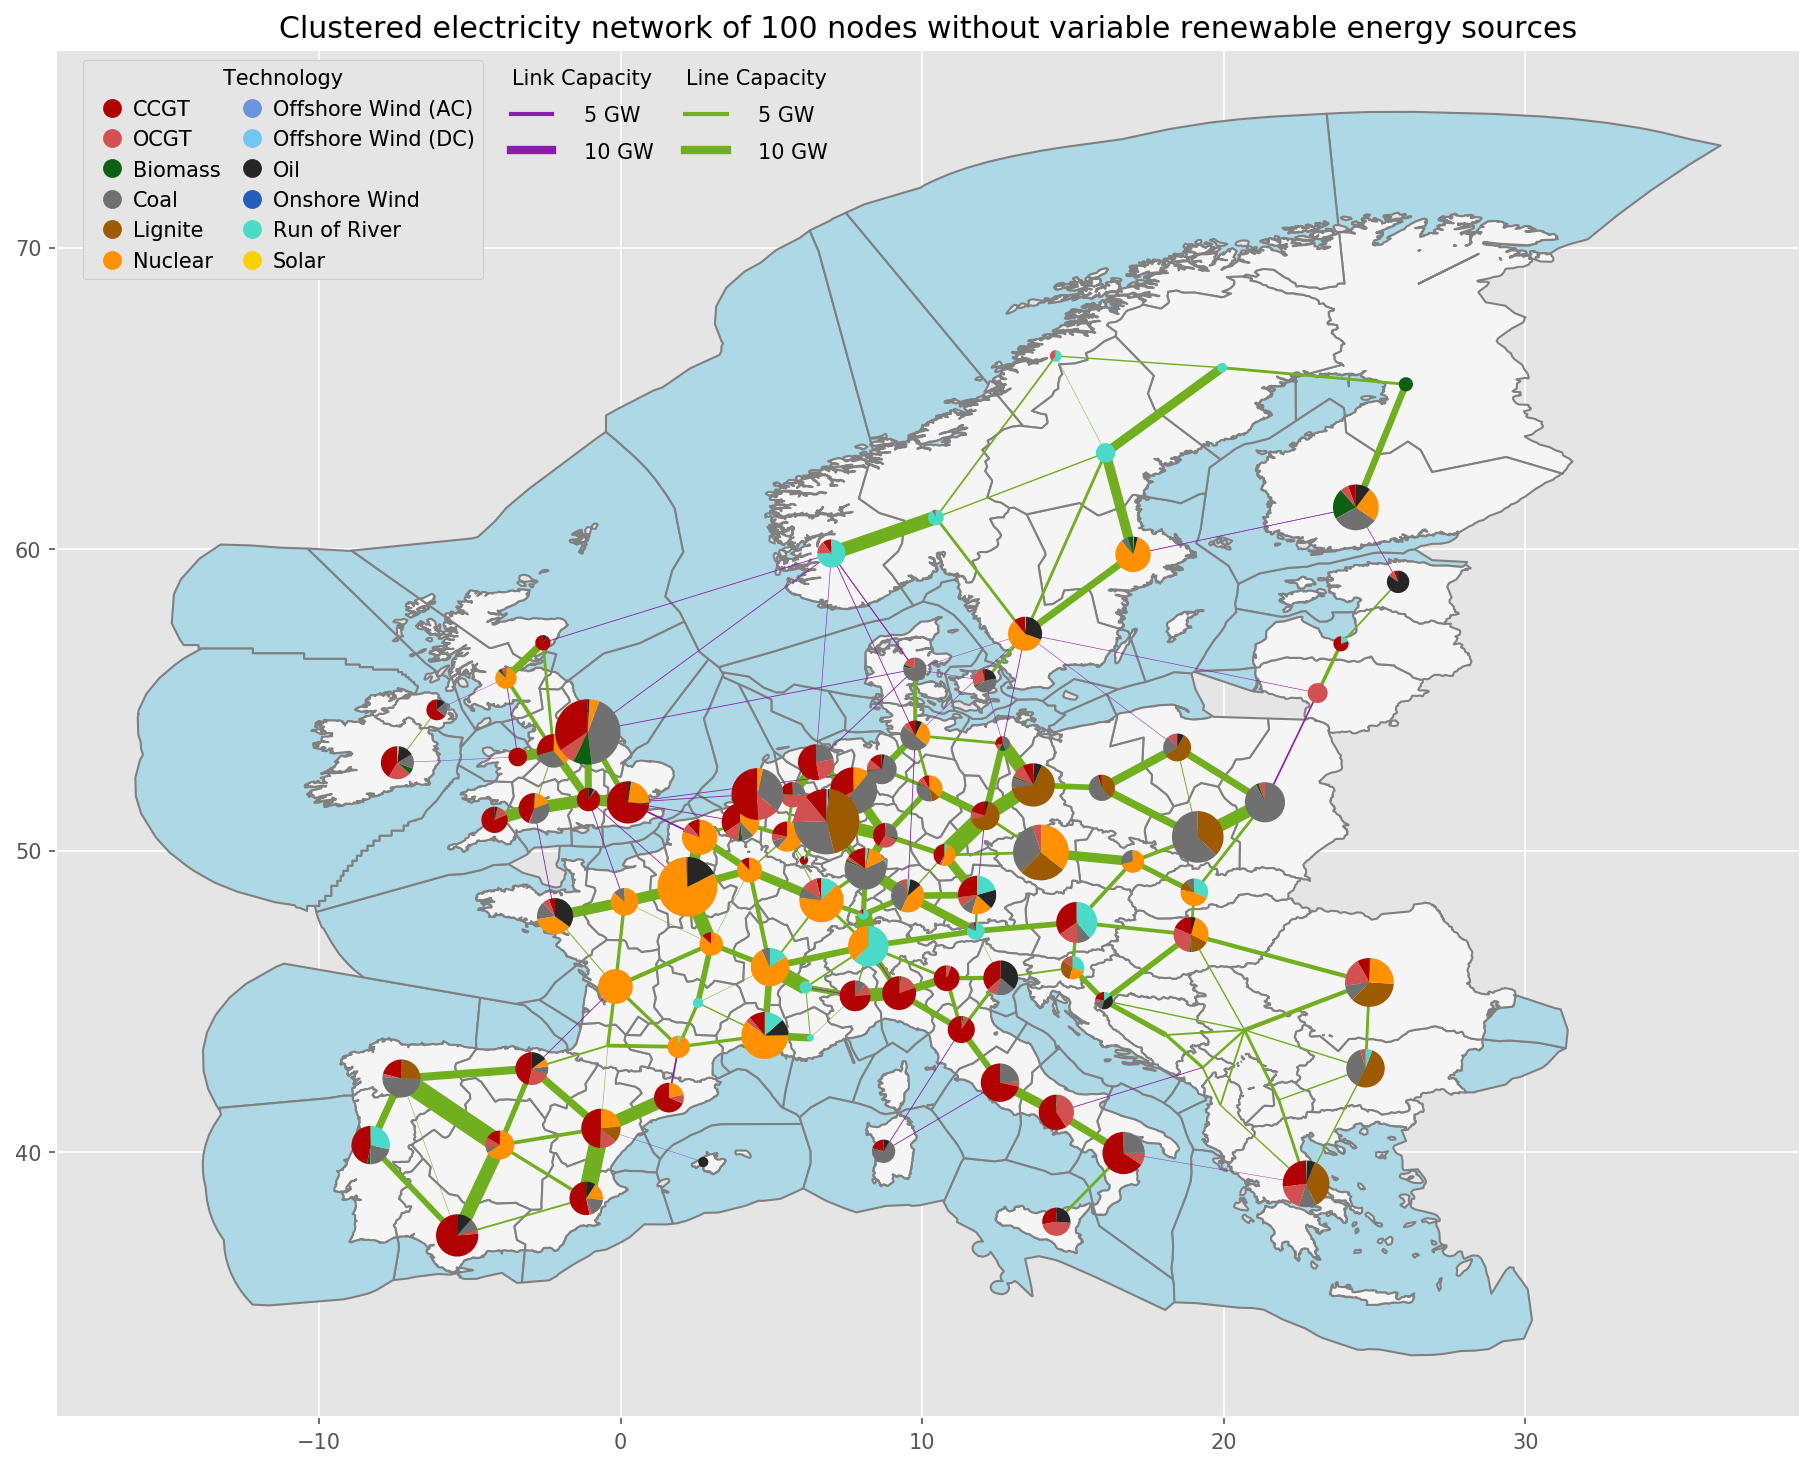
\includegraphics[width=8cm]{images/elec_s_100.png}
  \end{column}
  \end{columns}

  \source{Image: \href{https://github.com/PyPSA/pypsa-eur}{github.com/PyPSA/pypsa-eur}}
\end{frame}



\begin{frame}{Mathematical model of 24/7 CFE procurement}

  {\footnotesize
  \begin{itemize}
  \item The mathematical model of 24/7~CFE procurement is based on the former work of authors: \hrefc{https://zenodo.org/record/7180097}{System-level impacts of 24/7 carbon-free electricity procurement in Europe} published in October 2022. The study included mathematics additional to the PyPSA-Eur model to encode a situation when a fraction of C\&I consumers in a selected European countries commit to the 24/7~CFE goals. The resulting problem optimized investment and operational decisions to meet projected electricity demand for the 24/7~CFE consumers, as well as the demand of other consumers in the European electricity system, while meeting all relevant engineering, reliability, and policy constraints.
  
  \item In this study, we enhance the mathematical model of 24/7~CFE procurement by considering demand flexibility provided by data centers. The load flexibility involves \alert{temporal} (computing jobs scheduling) and \alert{spatial} (computing jobs migration) load shifting. 

  \item Thus, a data center operator (i.e., a flexible consumer following 24/7~CFE goal) can meet a given CFE target by either procuring energy generation and storage assets directly, and buying electricity from a local grid in hours when electricity mix is sufficiently clean  (like in the previous study), as well as utilize spatial and/or temporal flexibility to achieve hourly matching of demand with clean electricity more efficiently.
  \end{itemize}
  }
\end{frame}



\begin{frame}{Matching electricity supply and demand: a case of inflexible consumer}

  {\footnotesize
  The model optimizes a portfolio of carbon-free generation and storage technologies 
  procured by the C\&I consumers that commit to 24/7~CFE goal. The portfolio assets have to be located in the same market zone.

  The hourly demand of 24/7 participating consumer $d_t$ for hour $t$ can be met by a combination of the following: \\
    \begin{itemize}
      \item dispatch $g_{r,t}$ of procured carbon-free generators $r\in CFE$ 
      \item dispatch $\bar{g}_{s,t}$ of procured storage technologies $s\in STO$
            (requires charge $\ubar{g}_{s,t}$)
      \item imports of electricity from the grid $im_t$.
    \end{itemize}

  \begin{columns}
  \begin{column}{8cm}
  \begin{equation}
  \sum_{r\in CFE} g_{r,t} + \sum_{s\in STO} \left(\bar{g}_{s,t} - \ubar{g}_{s,t}\right) - ex_t + im_t  =  d_t \hspace{.7cm} \forall t
  \label{eqn:inflexnb}
  \end{equation}

  \vspace{0.3cm}
  NB: the excess from the local supply $ex_t$ can either be sold to the grid at market prices or curtailed.
  \end{column}

\begin{column}{5cm}
\centering
{\small
\begin{circuitikz}
  \draw (0,13.5) to [short,i^=$im_t$]  (1.5,13.5) to (1.5,13);
  \draw [ultra thick] (0,13) node[anchor=south]{} -- (4,13);
  \draw(2.5,13) |- +(0,0.5) to [short,i^=$ex_t$] +(1.5,0.5);
  \draw (0.5,13) -- +(0,-0.5) node[sground]{};
  \draw (2,12) node[vsourcesinshape, rotate=270](V2){}
  (V2.left) -- +(0,0.6);
  \draw (3.5,13) -- (3.5,12.4);
  \draw (3.5,12.4) to [esource] (3.5,11.7);
  \draw (0.5,11.3) node{$d_t$};
  \draw (2,11.3) node{$g_{CFE,t}$};
  \draw (3.5,11.3) node{$g_{STO,t}$};
\end{circuitikz}
}
\end{column}
\end{columns}

}
\end{frame}



\begin{frame}{24/7 CFE matching: a case of inflexible consumer}

  {\footnotesize

  The \alert{24/7 CFE matching} is modelled with a constraint (\ref{eqn:CFE}), 
  which matches demand of participating consumers with carbon-free resources on an hourly basis.  The constraint ensures that sum over generators from procured CFE resources $r\in CFE$, discharge and charge from storage technologies $s\in STO$,
  as well as import from the grid $im_t$ multiplied by the grid's CFE factor $CFE_t$
  must be higher or equal than a certain \alert{CFE score} $x$ multiplied with the total load $d_t$:
  \vspace{0.1cm}
  \begin{equation}
  \sum_{r\in CFE, t\in T} g_{r,t} + \sum_{s\in STO, t\in T} \left(\bar{g}_{s,t} - \ubar{g}_{s,t}\right) - \sum_{t\in T} ex_t + \sum_{t\in T} CFE_t \cdot im_t \geq x \cdot \sum_{t\in T} d_t
  \label{eqn:CFE}
  \end{equation}

  \vspace{0.3cm}

  \begin{columns}[T]
    \begin{column}{7.5cm}
    \centering  
    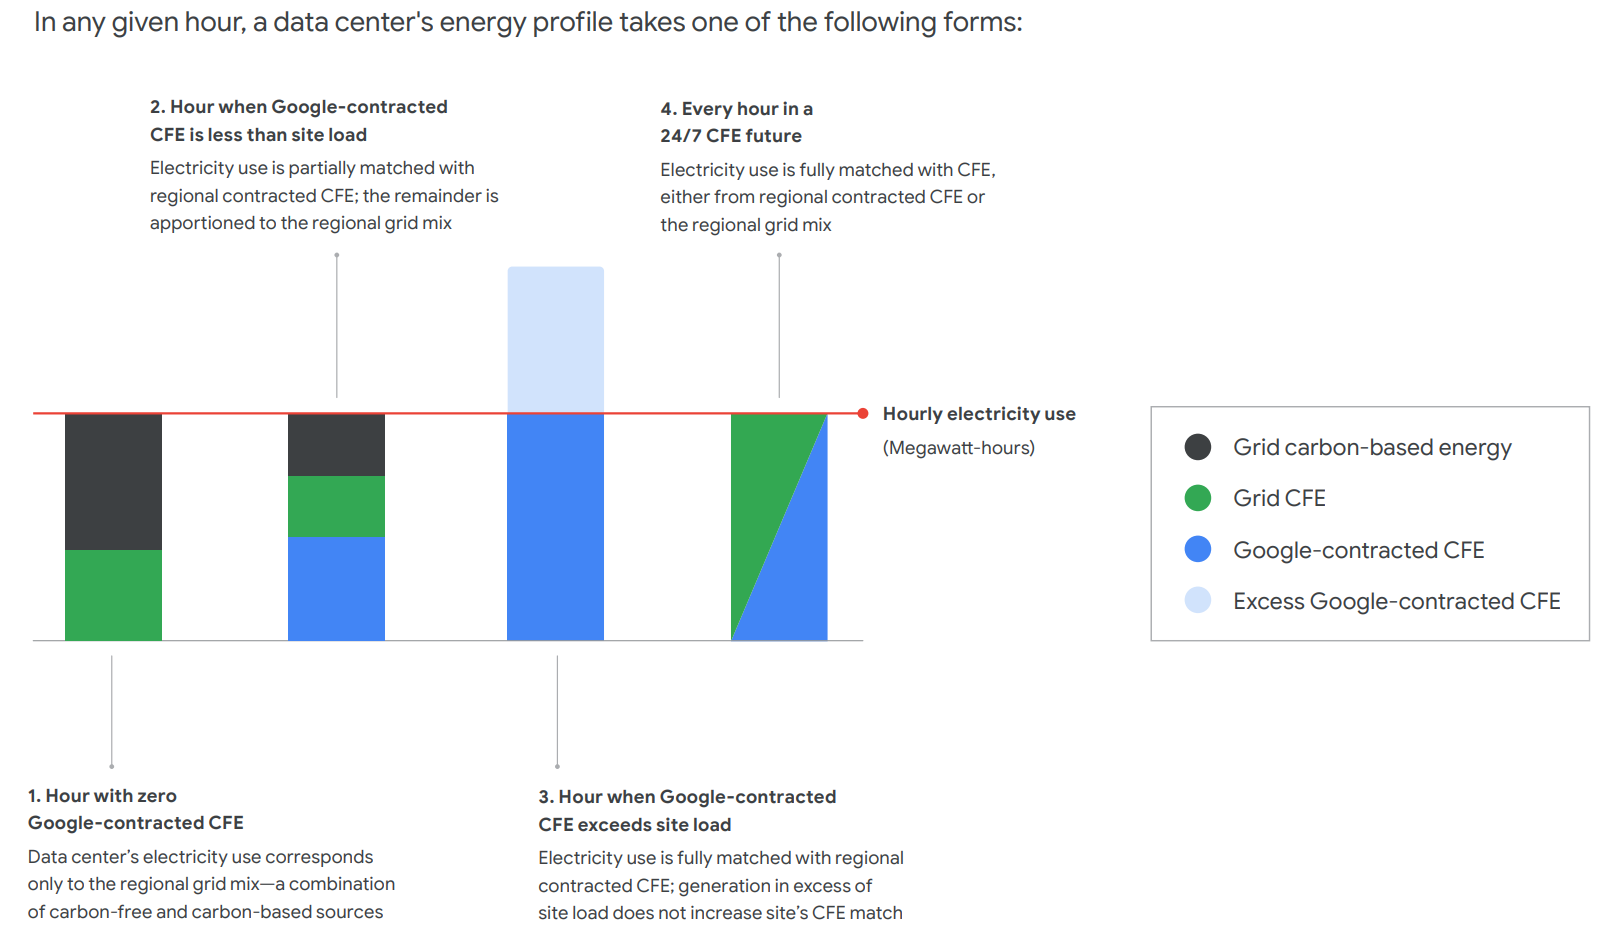
\includegraphics[width=8cm]{images/247-concept.png}
    \end{column}
    \begin{column}{6cm}
    \vspace{0.3cm}
      \noindent\fbox{%
      \parbox{\textwidth}{%
    The \alert{CFE score} $x$~[\%] measures the degree to which hourly electricity consumption is matched with carbon-free electricity generation within the regional grid.
    The matric is calculated using both CFE contracted by 24/7 participant, as well as CFE coming from the regional grid mix. \\
    \\
    The 24/7 CFE matching concept is aligned with \hrefc{https://www.gstatic.com/gumdrop/sustainability/24x7-carbon-free-energy-methodologies-metrics.pdf}{24/7 CFE: Methodologies and Metrics} paper by Google.
    }} 

    \end{column}
    \end{columns}
    }
\source{Image: \href{https://www.gstatic.com/gumdrop/sustainability/24x7-carbon-free-energy-methodologies-metrics.pdf}{24/7 CFE: Methodologies and Metrics}, Google 2021}    
\end{frame}


\begin{frame}{24/7 CFE matching: grid CFE factor}

  {\footnotesize

  The \alert{grid CFE factor} $CFE_t$ in eq. (\ref{eqn:CFE}) defines the percentage of clean electricity in each MWh of imported electricity from the grid to supply participating 24/7 loads in a given hour. The factor depends on the generation mix in the region where 24/7 participant is located, as well as on the generation mix in other regions from which electricity is imported to the local region ($import_t$).

  \begin{columns}
    \begin{column}{8cm}
    Using notation on the right, the average cleanness of the rest of the electricity system is:   
  \begin{equation*}
  ImportCFE_t = \frac{A_t}{A_t + D_t}
  \end{equation*}

  The CFE factor of grid supply\footnote{\scriptsize{Generators contracted by 24/7 consumers (C) are excluded from the grid supply.}} for a given hour $t$ is:

  \begin{equation*}
  CFE_t = \frac{B_t + ImportCFE_t * import_t}{B_t + E_t + import_t}
  \end{equation*}    

  \end{column}
  \begin{column}{5cm}
  \centering
  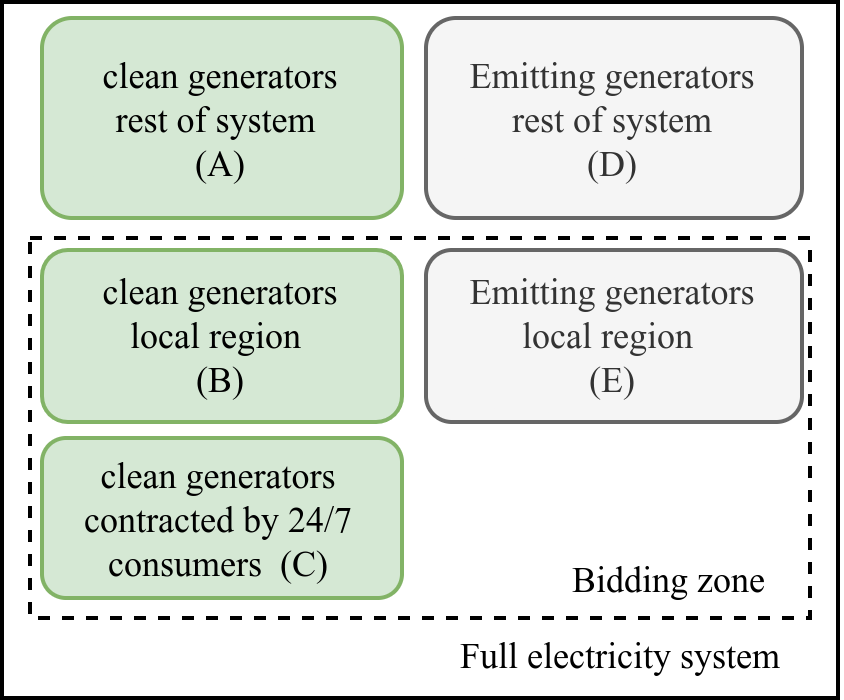
\includegraphics[width=4.5cm]{images/cfe.png} \\
  \scriptsize{Here we follow \hrefc{https://acee.princeton.edu/24-7/}{Xu et al. (2021)}}
  \end{column}
    
  \end{columns}
  \noindent\fbox{%
  \parbox{\textwidth}{%
  \scriptsize{
  Note that the grid CFE factor is affected by capacity procured by 24/7 consumers. This
  introduces a nonconvex term to the optimization problem. The nonconvexity can be avoided by treating the grid CFE factor as a parameter that is iteratively updated (starting with $CFE_t =0 \,~\forall t$). In the previous study, we concluded that one forward pass (i.e. 2 iterations) yields very good convergence. This observation holds true also for the optimization problem behind this study with multiple 24/7 consumers.}
  }}
  }
\end{frame}


\begin{frame}{24/7 CFE matching: excess CFE}

  {\footnotesize

  The \alert{excess CFE} represents generation from the procured resources above consumption of the 24/7 participant in a particular hour.  The excess CFE \alert{is not counted toward the CFE score} -- and thus it is subtracted on the left-hand side of the eq. (\ref{eqn:CFE}). While it does not contribute to the CFE Score, excess CFE could potentially be stored (using batteries) and shifted to another hour, sold to the regional grid at {\bf market prices}, or curtailed. 

  \vspace{0.2cm}

  The total amount of CFE exported to the regional grid is constrained to a certain level on an annual basis. The export limit ($ExLimit$) is set to 20\% of annual 24/7 participating consumer's demand. 
  Thus, constraint (\ref{eqn:excess}) gives the 24/7 participant flexibility to sell electricity to the regional grid, while avoiding the situation that sales to the grid become significantly larger than CFE supply to own demand.
  
  \begin{equation}
  \sum_{t\in T} export_t \leq ExLimit \cdot \sum_{t\in T} d_t
  \label{eqn:excess}
  \end{equation}

  \vspace{0.2cm}
  \noindent\fbox{%
  \parbox{\textwidth}{%
  The {\bf market prices} are derived from the dual variable of each zone's
  \hrefc{https://pypsa.readthedocs.io/en/latest/components.html}{energy balance constraint}. An infinitely small relaxation of the constraint, i.e., one unit of load less to be met, returns the marginal costs of providing that unit, which can be used as the electricity price indicator in a competitive market.
  }}
  }

\end{frame}



%%%%%%%%%%%%%%%%%%%%%%%%%%%%%%%%%%%%%%%%%%%%%%%%%%%%%%%%%%%%%%%%%%%%%%%
\begin{frame}{Spatial load shifting problem 1/3}

  {\footnotesize

  We introduce a concept of \alert{spatial load management system} that allows for shifting load across locations. The load shifts take place via \alert{virtual links} -- non-physical pathways between data centers (\href{https://doi.org/10.1016/j.apenergy.2022.119930}{Zhang \& Zavala~(2022)}).

  \centering
  \vspace{-0.2cm}
  \hspace*{0.5cm}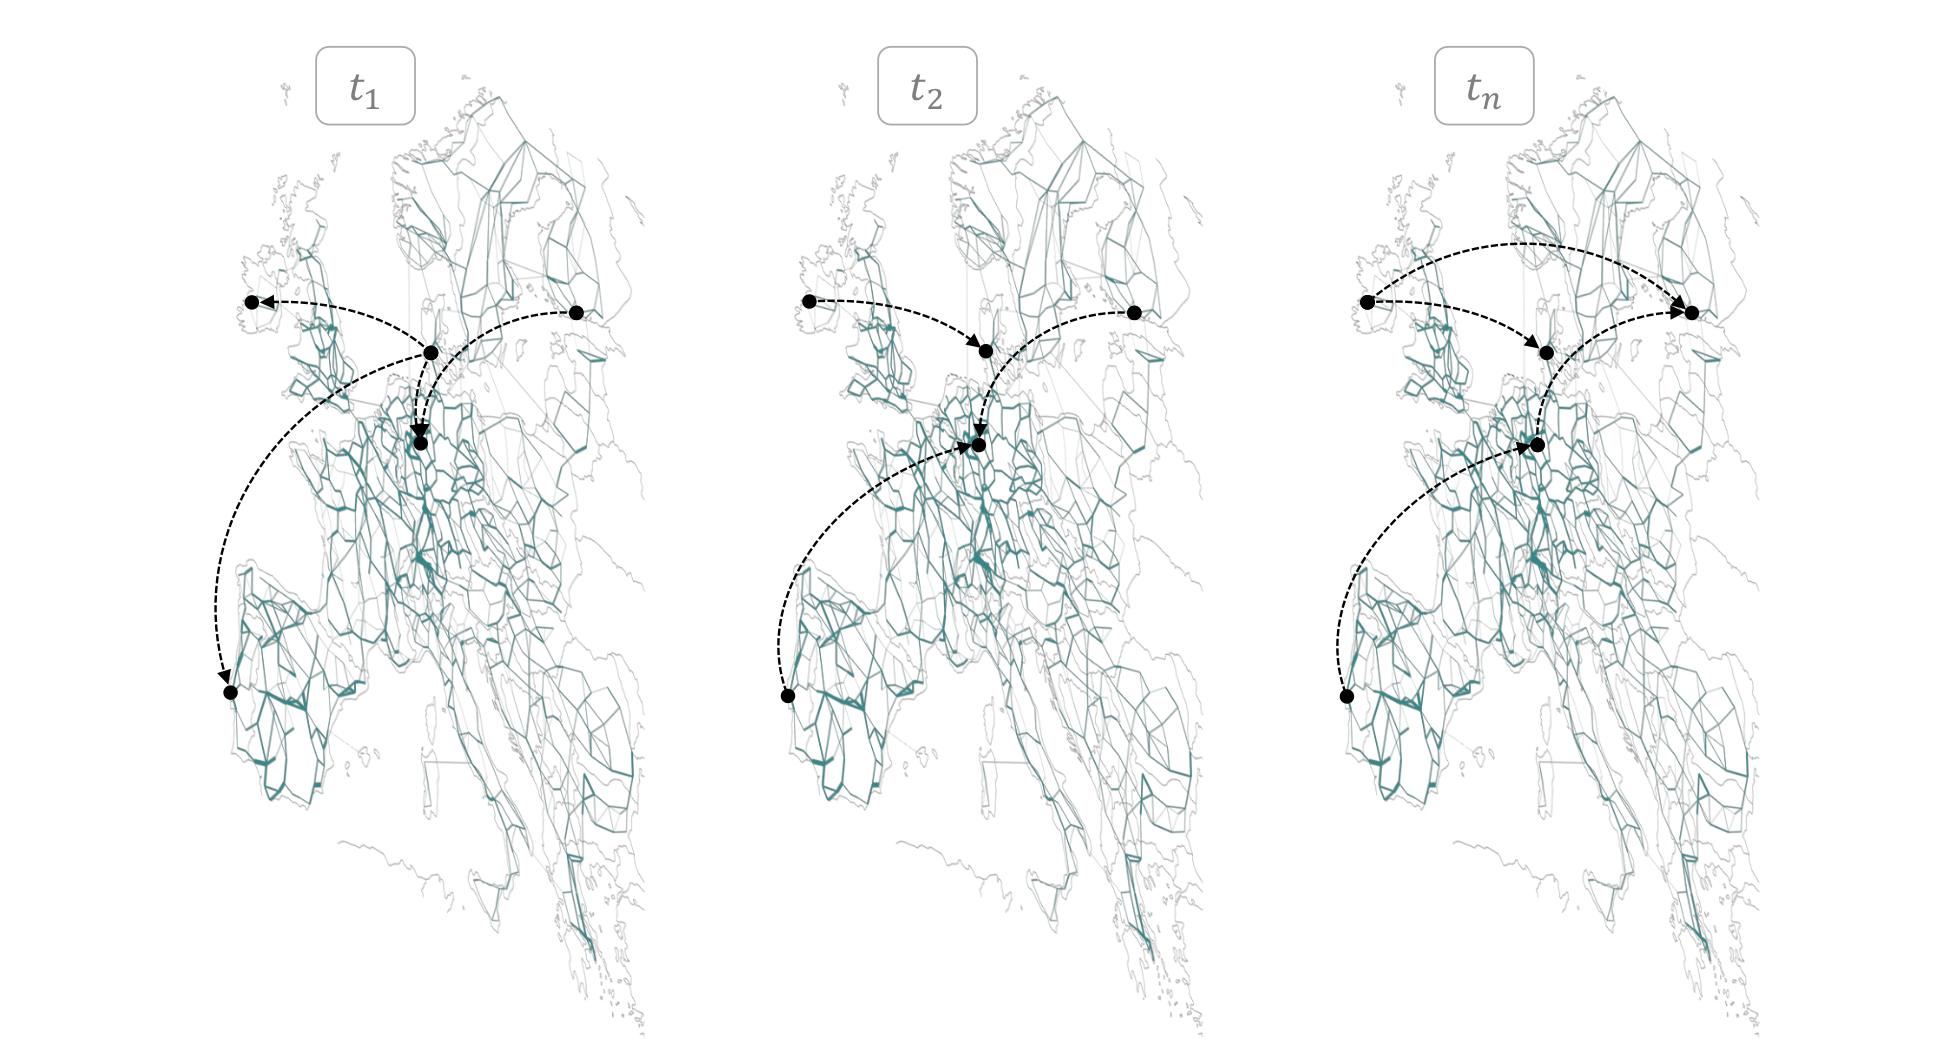
\includegraphics[width=13cm]{images/spatial-vlinks.png}
  }
\end{frame}


\begin{frame}{Spatial load shifting problem 2/3}

  {\footnotesize

  We introduce a concept of \alert{spatial load management system} that allows for shifting workloads across locations. The load shifts take place via \alert{virtual links} -- non-physical pathways between data center nodes (\href{https://doi.org/10.1016/j.apenergy.2022.119930}{Zhang \& Zavala (2022)}).

  Let $\Theta$ be the set of all virtual links; let $\delta_\vartheta \in \mathbb{R}_{+}$ be load shifts (flows via virtual pathways); and let $N_{DC}$ be the set of data centers (flexible consumers). We can define $\Theta_n^{snd} := \{\vartheta \in \Theta | snd(\vartheta) = n\} \subseteq \Theta$, $\Theta_n^{rec} := \{\vartheta \in \Theta | rec(\vartheta) = n\} \subseteq \Theta$ to be the set of sending and receiving virtual links at node $n \in N_{DC}$. 

  The nodal energy balance defined for inflexible consumers (eq.~\ref{eqn:inflexnb}) is now extended by variables representing shifts of load \alert{across locations}, since the dispatched load at a given node can include shifts to/from other data center nodes: 

  \begin{columns}
    \begin{column}{8cm}
      \begin{equation}
        \begin{split}
     & \sum_{r\in CFE} g_{r,n,t} + \sum_{s\in STO} \left(\bar{g}_{s,n,t} - \ubar{g}_{s,n,t}\right) - ex_{n,t} + im_{n,t}  = \\
     & \textcolor{TUred}{d_{n,t} + \sum_{\vartheta \in \Theta_n^{rec}}\delta_{\vartheta, t} - \sum_{\vartheta \in \Theta_n^{snd}}\delta_{\vartheta, t}} \hspace{.5cm} \forall n \in N_{DC}, t \in T 
        \end{split}
      \label{eqn:spatialnb}
      \end{equation}
    \end{column}
  \begin{column}{5cm}
  \centering
  {\small
  \begin{circuitikz}
    \draw (0,13.5) to [short,i^=$im_{n,t}$]  (1.5,13.5) to (1.5,13);
    \draw [ultra thick] (0,13) node[anchor=south]{} -- (4,13);
    \draw(2.5,13) |- +(0,0.5) to [short,i^=$ex_{n,t}$] +(1.5,0.5);
    \draw (0.5,13) -- +(0,-0.5) node[sground]{};
    \draw (2,12) node[vsourcesinshape, rotate=270](V2){}
    (V2.left) -- +(0,0.6);
    \draw (3.5,13) -- (3.5,12.4);
    \draw (3.5,12.4) to [esource] (3.5,11.7);
    \draw (0.5,11.3) node{\textcolor{TUred}{$\widetilde{d}_{n,t}$}};
    \draw (2,11.3) node{$g_{CFE,n,t}$};
    \draw (3.5,11.3) node{$g_{STO,n,t}$};
  \end{circuitikz}
  }
  \end{column}
  \end{columns}
  }
\end{frame}


\begin{frame}{Spatial load shifting problem 3/3}

  {\footnotesize
  \begin{columns}

    \begin{column}{6cm}
      Computing capacity constraints (eq. \ref{eqn:spatialflex}) ensure that the dispatched load at each data center  $\widetilde{d}_{n,t}$ does not exceed available capacity (an upper limit, eq. \ref{eqn:spatialb}), as well as that a certain data center does not shift load that exceeds flexible jobs share (a lower limit, eq. \ref{eqn:spatialc}).
    \end{column}

  \begin{column}{7cm}
    \begin{subequations}
      \begin{align}
          \widetilde{d}_{n,t} &=  d_{n,t} + \sum_{\vartheta \in \Theta_n^{rec}}\delta_{\vartheta, t} - \sum_{\vartheta \in \Theta_n^{snd}}\delta_{\vartheta, t} \quad \forall n \in N_{DC}, t \in T \label{eqn:spatiala} \\
          \widetilde{d}_{n,t} &\le [1+f] \cdot d_{n,t}  \quad \forall n \in N_{DC}, t \in T \label{eqn:spatialb} \\
          \widetilde{d}_{n,t} &\ge [1-f] \cdot d_{n,t}  \quad \forall n \in N_{DC}, t \in T \label{eqn:spatialc}
      \end{align}
      \label{eqn:spatialflex}
      \end{subequations}
  \end{column}
  \end{columns}

  \vspace{-0.1cm}
  NB spatial load shifts are not subject to any electricity network transmission constraints; as such, the only source of congestion for the virtual links is computing capacity constraints (i.e., availability of flexible workloads). \\

  \vspace{0.1cm}
  The 24/7~CFE matching constraint for inflexible consumer (eq. \ref{eqn:CFE}) is now defined over a set of data center nodes $n \in N_{DC}$ and is extended on the right-hand side by spatial load shifts. Thus, flexible consumer can benefit from an additional degree of freedom that helps relaxing the constraint for locations and times when providing demand with carbon-free electricity is difficult:
  \vspace{0.1cm}
  \begin{equation}
    \begin{split}
  &\sum_{r\in CFE, t\in T} g_{r,n,t} + \sum_{s\in STO, t\in T} \left(\bar{g}_{s,n,t} - \ubar{g}_{s,n,t}\right) - \sum_{t\in T} ex_{n,t} + \sum_{t\in T} CFE_{n,t} \cdot im_{n,t} \geq \\ 
  &x_n \cdot \textcolor{TUred}{\sum_{t\in T} \left( d_{n,t} + \sum_{\vartheta \in \Theta_n^{rec}}\delta_{\vartheta, t} - \sum_{\vartheta \in \Theta_n^{snd}}\delta_{\vartheta, t}\right)} \quad \forall n \in N_{DC} \label{eqn:spatialCFE}
    \end{split}
  \end{equation}
  }
  
\end{frame}


%%%%%%%%%%%%%%%%%%%%%%%%%%%%%%%%%%%%%%%%%%%%%%%%%%%%%%%%%%%%%%%%%%%%%%%
\begin{frame}{Temporal load shifting problem 1/3}

  {\footnotesize

  To capture temporal flexibility, we introduce a concept a data center \alert{temporal load management system} that allows for shifting load from a given time to another time point in the future.

  \centering
  \vspace{-0.2cm}
  \hspace*{0.5cm}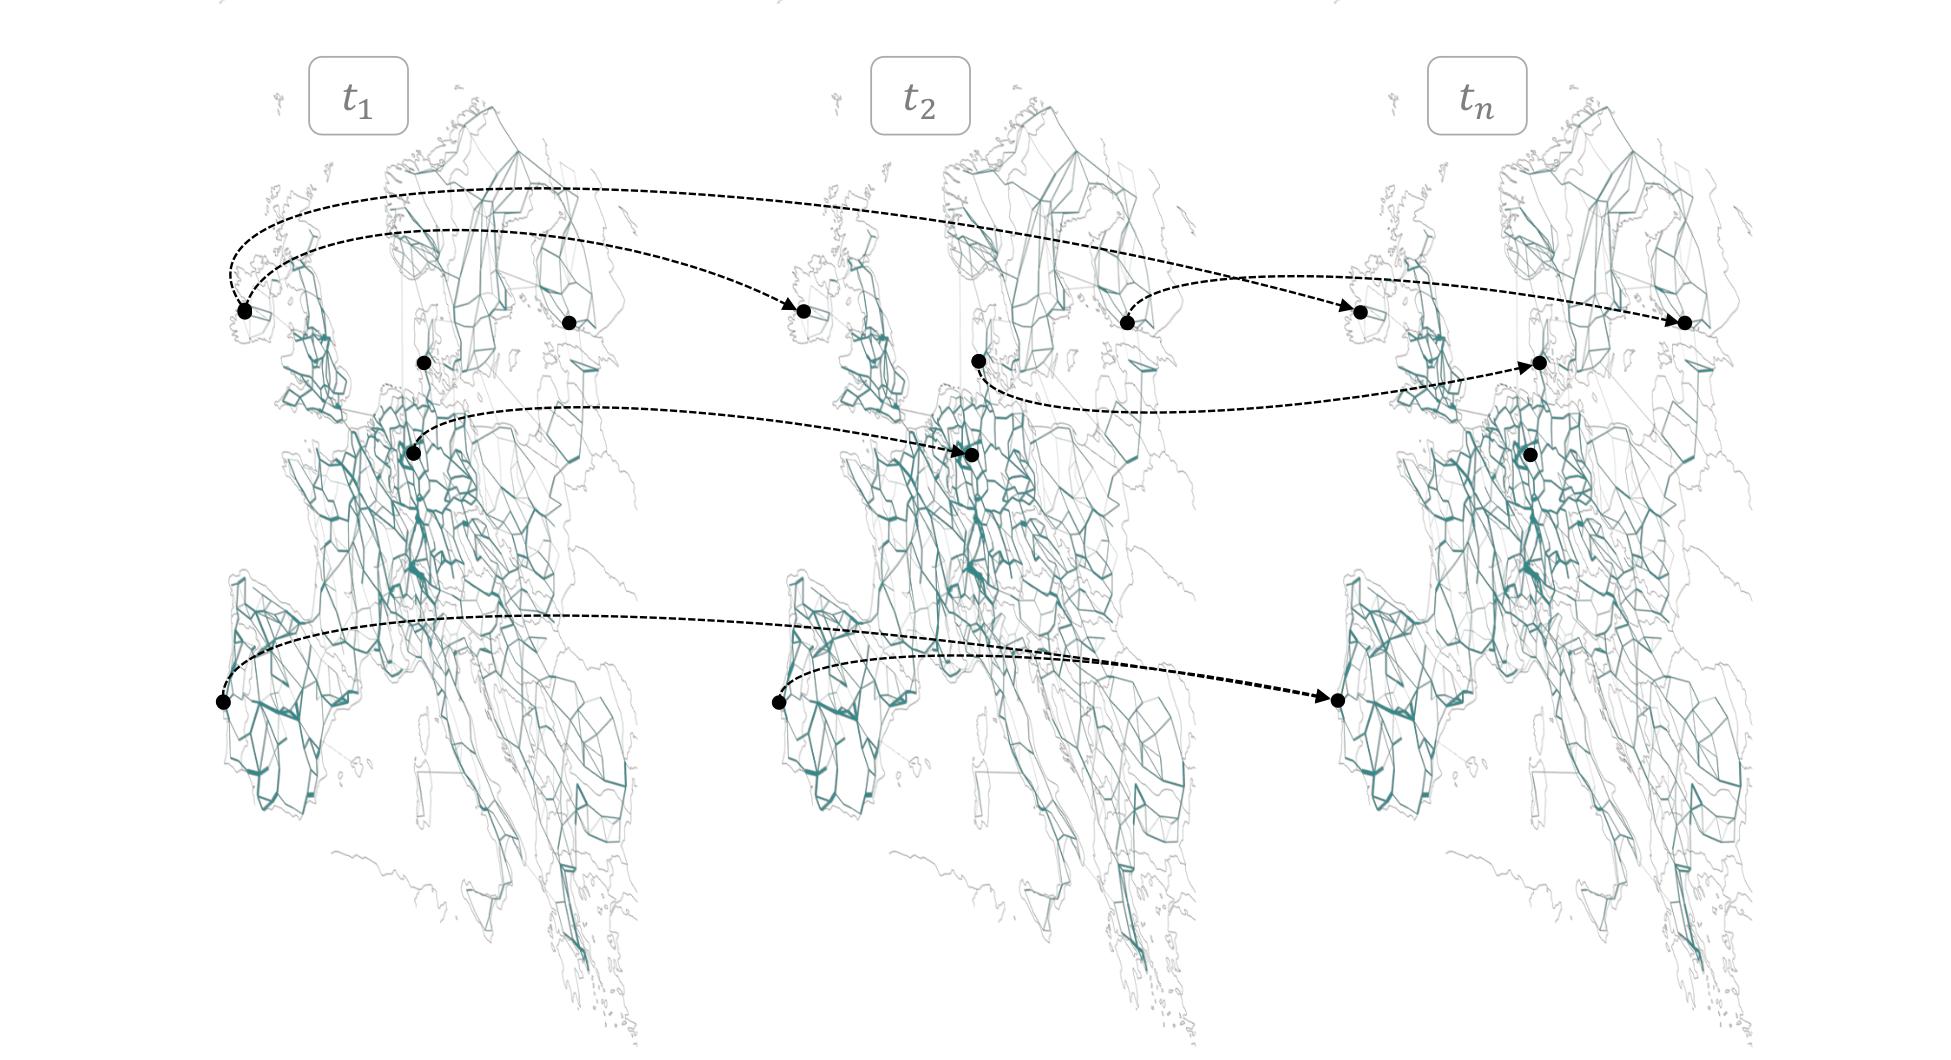
\includegraphics[width=13cm]{images/temporal-vlinks.png}
  }
\end{frame}


\begin{frame}{Temporal load shifting problem 2/3}

  {\footnotesize

  To capture temporal flexibility, we introduce a concept a data center \alert{temporal load management system} that allows for shifting load from a given time to another time point in the future.

  Consider a time horizon of our optimization problem $T = \{t_1 , t_2 , ..., t_T\}$. For simplicity, let us assume that there is a single flexible consumer (i.e., no spatial load shifts) with a demand-side temporal load management mechanism denoted with a singleton set $\{s'\}$. Let variables $\bar{g}_{s',t},\ubar{g}_{s',t} \in \mathbb{R}_{+}$ be workloads that are resheduled in time, i.e., shifted from a time $t$ to a later time $t'$. Thus, the dispatched load  $\widetilde{d_{t}}$ of flexible consumer can deviate from the nominal value $d_{n,t}$ due to temporal load management. 
  
  The nodal energy balance is now extended with variables representing shifts of load \alert{across time}:

  \begin{columns}
    \begin{column}{8cm}
      \begin{equation}
        \begin{split}
        &\sum_{r\in CFE} g_{r,t} + \sum_{s\in STO} \left(\bar{g}_{s,t} - \ubar{g}_{s,t}\right) - ex_{t} + im_{t}  = \\
        &\textcolor{TUred}{d_{t} + \sum_{{s'}} \left(\bar{g}_{s',t} - \ubar{g}_{s',t}\right)}\hspace{.5cm} \{N_{DC}\}, \forall t \in T 
        \label{eqn:temporalnb}
        \end{split}
      \end{equation}
      \end{column}
  \begin{column}{5cm}
  \centering
  {\small
  \begin{circuitikz}
    \draw (0,13.5) to [short,i^=$im_{t}$]  (1.5,13.5) to (1.5,13);
    \draw [ultra thick] (0,13) node[anchor=south]{} -- (4,13);
    \draw(2.5,13) |- +(0,0.5) to [short,i^=$ex_{t}$] +(1.5,0.5);
    \draw (0.5,13) -- +(0,-0.5) node[sground]{};
    \draw (2,12) node[vsourcesinshape, rotate=270](V2){}
    (V2.left) -- +(0,0.6);
    \draw (3.5,13) -- (3.5,12.4);
    \draw (3.5,12.4) to [esource] (3.5,11.7);
    \draw (0.5,11.3) node{\textcolor{TUred}{$\widetilde{d_{t}}$}};
    \draw (2,11.3) node{$g_{CFE,t}$};
    \draw (3.5,11.3) node{$g_{STO,t}$};
  \end{circuitikz}
  }
  \end{column}
  \end{columns}
  }
\end{frame}


\begin{frame}{Temporal load shifting problem 3/3}

  {\footnotesize
  \begin{columns}

    \begin{column}{7.2cm}
      Computing capacity constraints for temporal load shifting problem (eq. \ref{eqn:temporalflex}) ensure that workloads delayed to a given time $t$ do not exceed available cluster capacity (an upper limit, eq. \ref{eqn:temporalb}), as well as that only flexible workloads can be shifted in time (a lower limit, eq. \ref{eqn:temporalc}).
    \end{column}

  \begin{column}{5.8cm}
  \begin{subequations}
    \begin{align}
        \widetilde{d_{t}} =  d_{t} + \sum_{{s'}} \left(\bar{g}_{s',t} - \ubar{g}_{s',t}\right)\quad &\forall t \in T  \label{eqn:temporala} \\
        \widetilde{d_{t}} \le [1+f] \cdot d_{t}  \quad &\forall t \in T  \label{eqn:temporalb} \\
        \widetilde{d_{t}} \ge [1-f] \cdot d_{t}  \quad &\forall t \in T  \label{eqn:temporalc}
    \end{align}
    \label{eqn:temporalflex}
    \end{subequations}
  \end{column}
  \end{columns}

  \vspace{-0.1cm}
  We follow \href{https://arxiv.org/abs/2106.11750}{Radovanovic et al. (2021)} implementing the daily usage conservation rule -- an additional constraint to ensure that the cluster-level daily compute usage is preserved when flexible workload is shifted in time:

  \begin{equation}
    \sum_{t | t \in t(DAYS)} \left(\bar{g}_{s',t} - \ubar{g}_{s',t}\right) = 0 \quad \{s'\}
    \label{eqn:dailyconserv}
  \end{equation}

  The 24/7~CFE matching constraint is also extended to account for the temporal load management mechanism. Consumer with temporally flexible demand benefits from an additional degree of freedom that helps achieving a CFE target by shifting load away from hours when matching demand with carbon-free electricity is expensive:
  \vspace{0.1cm}
  \begin{equation}
    \begin{split}
  &\sum_{r\in CFE, t\in T} g_{r,t} + \sum_{s\in STO, t\in T} \left(\bar{g}_{s,t} - \ubar{g}_{s,t}\right) - \sum_{t\in T} ex_{t} + \sum_{t\in T} CFE_{t} \cdot im_{t} \geq \\ 
  &x \cdot \textcolor{TUred}{\sum_{t\in T} \left( d_{t} + \sum_{{s'}}\left(\bar{g}_{s',t} - \ubar{g}_{s',t}\right)\right)} \hspace{.5cm} \{N_{DC}\} 
  \label{eqn:temporalCFE}
    \end{split}
  \end{equation}
  
  }
\end{frame}


%%%%%%%%%%%%%%%%%%%%%%%%%%%%%%%%%%%%%%%%%%%%%%%%%%%%%%%%%%%%%%%%%%%%%%%
\begin{frame}{Spatially-temporal load shifting problem 1/3}
  \centering
  \vspace{0.3cm}
  \hspace{-0.3cm}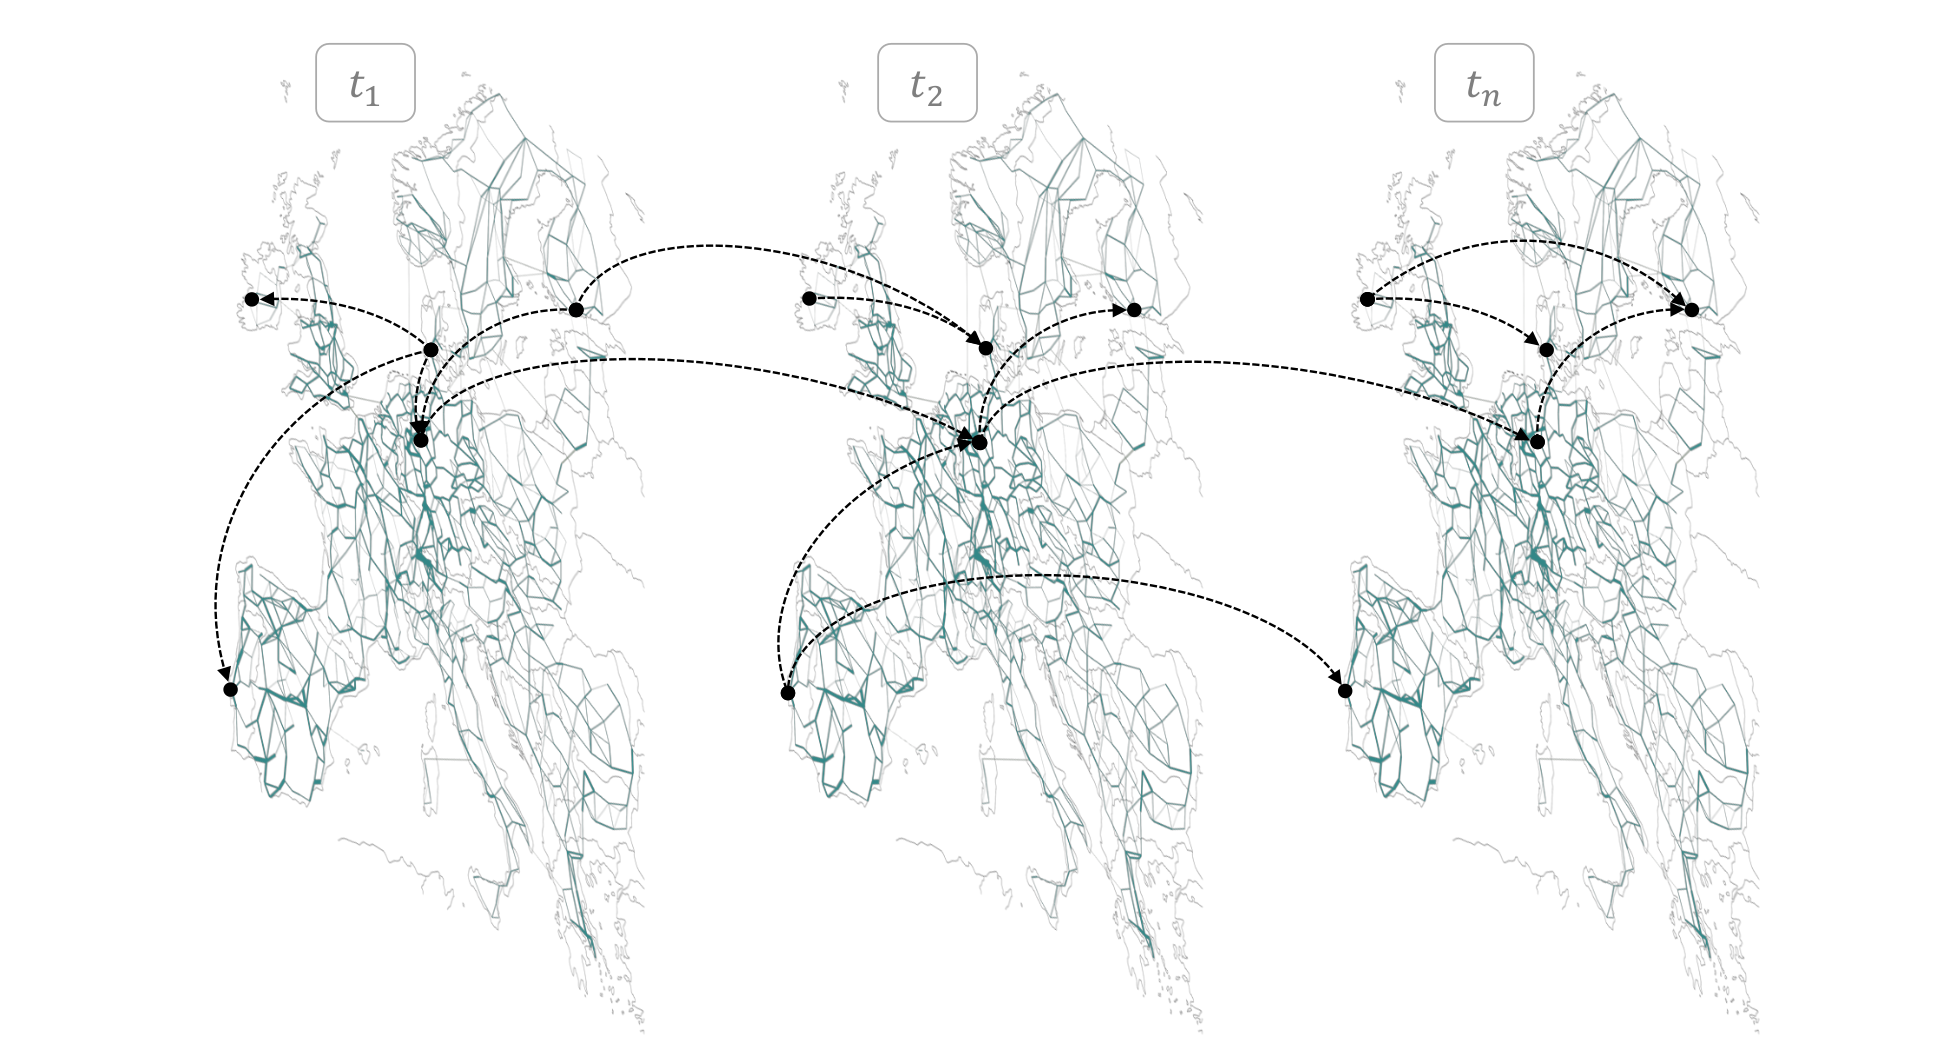
\includegraphics[width=13cm]{images/spatial-temporal-vlinks.png}
\end{frame}


\begin{frame}{Spatially-temporal load shifting problem 2/3}

  {\footnotesize

  The temporal and spatial flexibility of electricity demand can be \alert{co-optimized} to help achieve clean electricity targets. The resulting mathematical problem brings together the formulations of spatial and temporal load management systems shown above.

  We consider a set of data centers (flexible consumers) $n \in N_{DC}$ located in various locations within the electricity network. Data centers are interconnected with virtual links $\Theta_n^{snd}, \Theta_n^{rec}$ (complete graph). Each data center also has a temporal load management mechanism $S_n^{dsm} := \{s' \in S | dsm(s') = n\}$.

  The nodal energy balance is adjusted to account for variables representing load shifts \alert{across space and time}:

  \vspace{0.2cm}
  \begin{columns}
    \begin{column}{9cm}
      \begin{equation}
        \begin{split}
        &\sum_{r\in CFE} g_{r,n,t} + \sum_{s\in STO} \left(\bar{g}_{s,n,t} - \ubar{g}_{s,n,t}\right) - ex_{n,t} + im_{n,t}  = \\
        & \textcolor{TUred}{d_{n,t} + \sum_{\vartheta \in \Theta_n^{rec}}\delta_{\vartheta, t} - \sum_{\vartheta \in \Theta_n^{snd}}\delta_{\vartheta, t} + \sum_{{s'} \in S_n^{dsm}} \left(\bar{g}_{s',n,t} - \ubar{g}_{s',n,t}\right)} \\ 
        & \hspace{.5cm} \forall n \in N_{DC}, t \in T 
        \label{eqn:bothnb}
        \end{split}
      \end{equation}
    \end{column}
  \begin{column}{5cm}
  \centering
  {\small
  \begin{circuitikz}
    \draw (0,13.5) to [short,i^=$im_{n,t}$]  (1.5,13.5) to (1.5,13);
    \draw [ultra thick] (0,13) node[anchor=south]{} -- (4,13);
    \draw(2.5,13) |- +(0,0.5) to [short,i^=$ex_{n,t}$] +(1.5,0.5);
    \draw (0.5,13) -- +(0,-0.5) node[sground]{};
    \draw (2,12) node[vsourcesinshape, rotate=270](V2){}
    (V2.left) -- +(0,0.6);
    \draw (3.5,13) -- (3.5,12.4);
    \draw (3.5,12.4) to [esource] (3.5,11.7);
    \draw (0.5,11.3) node{\textcolor{TUred}{$\widetilde{d}_{n,t}$}};
    \draw (2,11.3) node{$g_{CFE,n,t}$};
    \draw (3.5,11.3) node{$g_{STO,n,t}$};

  \end{circuitikz}
  }
  \end{column}
  \end{columns}
  }
\end{frame}


\begin{frame}{Spatially-temporal load shifting problem 3/3}

  {\footnotesize
  \begin{columns}

    \begin{column}{5cm}
      Computing capacity constraints (eq.~\ref{eqn:bothflex}) now ensure that the dispatched load at each data center  $\widetilde{d}_{n,t}$ does not exceed the limits for each data center $n \in N_{DC}$ considering both spatial and temporal load shifts at each time point $t$.
    \end{column}

  \begin{column}{8cm}
    \begin{subequations}
      \begin{align}
        \begin{split}
          &\widetilde{d}_{n,t} =  d_{n,t} + \sum_{\vartheta \in \Theta_n^{rec}}\delta_{\vartheta, t} - \sum_{\vartheta \in \Theta_n^{snd}}\delta_{\vartheta, t} \\
          &+ \sum_{{s'} \in S_n^{dsm}} \left(\bar{g}_{s',n,t} - \ubar{g}_{s',n,t}\right) \quad \forall n \in N_{DC}, t \in T \\
        \end{split}
        \label{eqn:botha} \\
        &\widetilde{d}_{n,t} \le [1+f] \cdot d_{n,t}  \quad \forall n \in N_{DC}, t \in T \label{eqn:bothb} \\
        &\widetilde{d}_{n,t} \ge [1-f] \cdot d_{n,t}  \quad \forall n \in N_{DC}, t \in T \label{eqn:bothc}
      \end{align}
      \label{eqn:bothflex}
      \end{subequations}
  \end{column}
  \end{columns}

  The daily compute usage conservation rule is applied to each data center:
  \begin{equation}
    \sum_{t | t \in t(DAYS)} \left(\bar{g}_{s',t} - \ubar{g}_{s',t}\right) = 0 \quad \forall {s'} \in S_n^{dsm}
    \label{eqn:dailyconserv2}
  \end{equation}

  Finally, the 24/7~CFE matching constraint is adjusted accordingly. With co-optimization of temporal or spatial load shifting, flexibility can be harnessed to achieve clean electricity targets more efficiently:
  \vspace{0.1cm}
  \begin{equation}
    \begin{split}
  &\sum_{r\in CFE, t\in T} g_{r,n,t} + \sum_{s\in STO, t\in T} \left(\bar{g}_{s,n,t} - \ubar{g}_{s,n,t}\right) - \sum_{t\in T} ex_{n,t} + \sum_{t\in T} CFE_{n,t} \cdot im_{n,t} \geq \\ 
  &x_n \cdot \textcolor{TUred}{\sum_{t\in T} \left( d_{n,t} + \sum_{\vartheta \in \Theta_n^{rec}}\delta_{\vartheta, t} - \sum_{\vartheta \in \Theta_n^{snd}}\delta_{\vartheta, t} + \sum_{{s'} \in S_n^{dsm}} \left(\bar{g}_{s',n,t} - \ubar{g}_{s',n,t}\right)\right)}\quad \forall n \in N_{DC} \label{eqn:bothCFE}
    \end{split}
  \end{equation}
  }
  
\end{frame}



%----------------------------------------
%----------------------------------------

\section{Annex B: Tools and data sources}


\begin{frame}
  \frametitle{PyPSA: an energy modelling ecosystem}

\begin{columns}[T]
\begin{column}{7cm}

{\footnotesize
  \begin{itemize}
  \item \hrefc{https://pypsa.org/}{pypsa.org} project provides a free, user-friendly and performant model environment to support a smooth energy transition around the world. 
  \item The project includes individual packages that enable to go all the way from data processing (e.g., calculating renewable energy potentials or collecting energy assets data) to creating complex energy optimization problems. 
  \item All packages are build in a modular sense so that they may be used independently from each other but interact easily.
  \item PyPSA development and maintenance is coordinated by the Department of Energy Systems @ TU~Berlin \hrefc{https://www.tu.berlin/en/ensys/about-us}{(ENSYS)}.  
  \end{itemize}
}
\end{column}
\begin{column}{9cm}

\centering
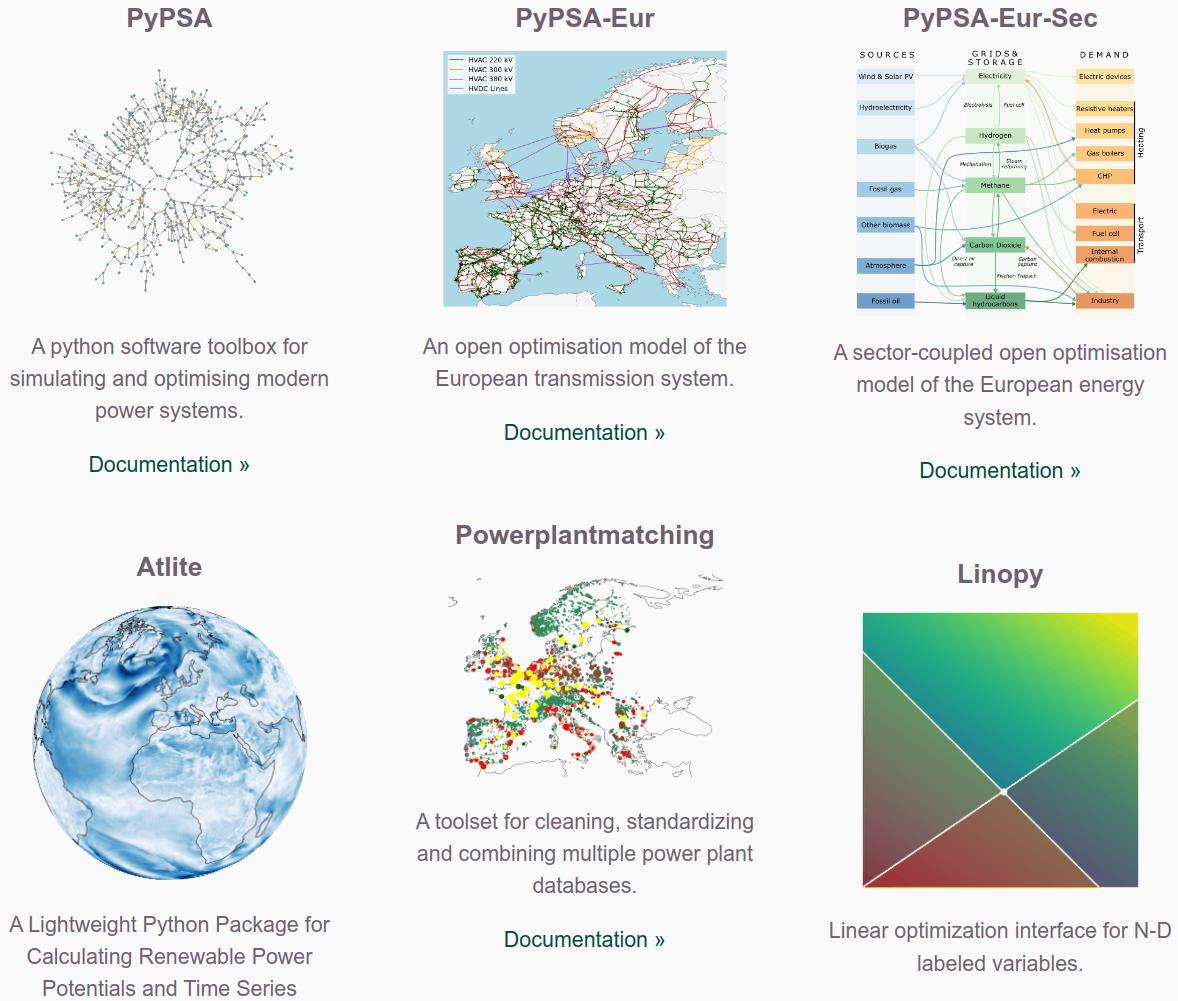
\includegraphics[width=8.5cm]{images/pypsa-web.png}
\source{\href{https://pypsa.org/}{Image: pypsa.org}}

\end{column}
\end{columns}

\end{frame}



\begin{frame}{Data sources: electricity grid}
 
  \begin{columns}[T]
  \begin{column}{6cm}

  \centering

  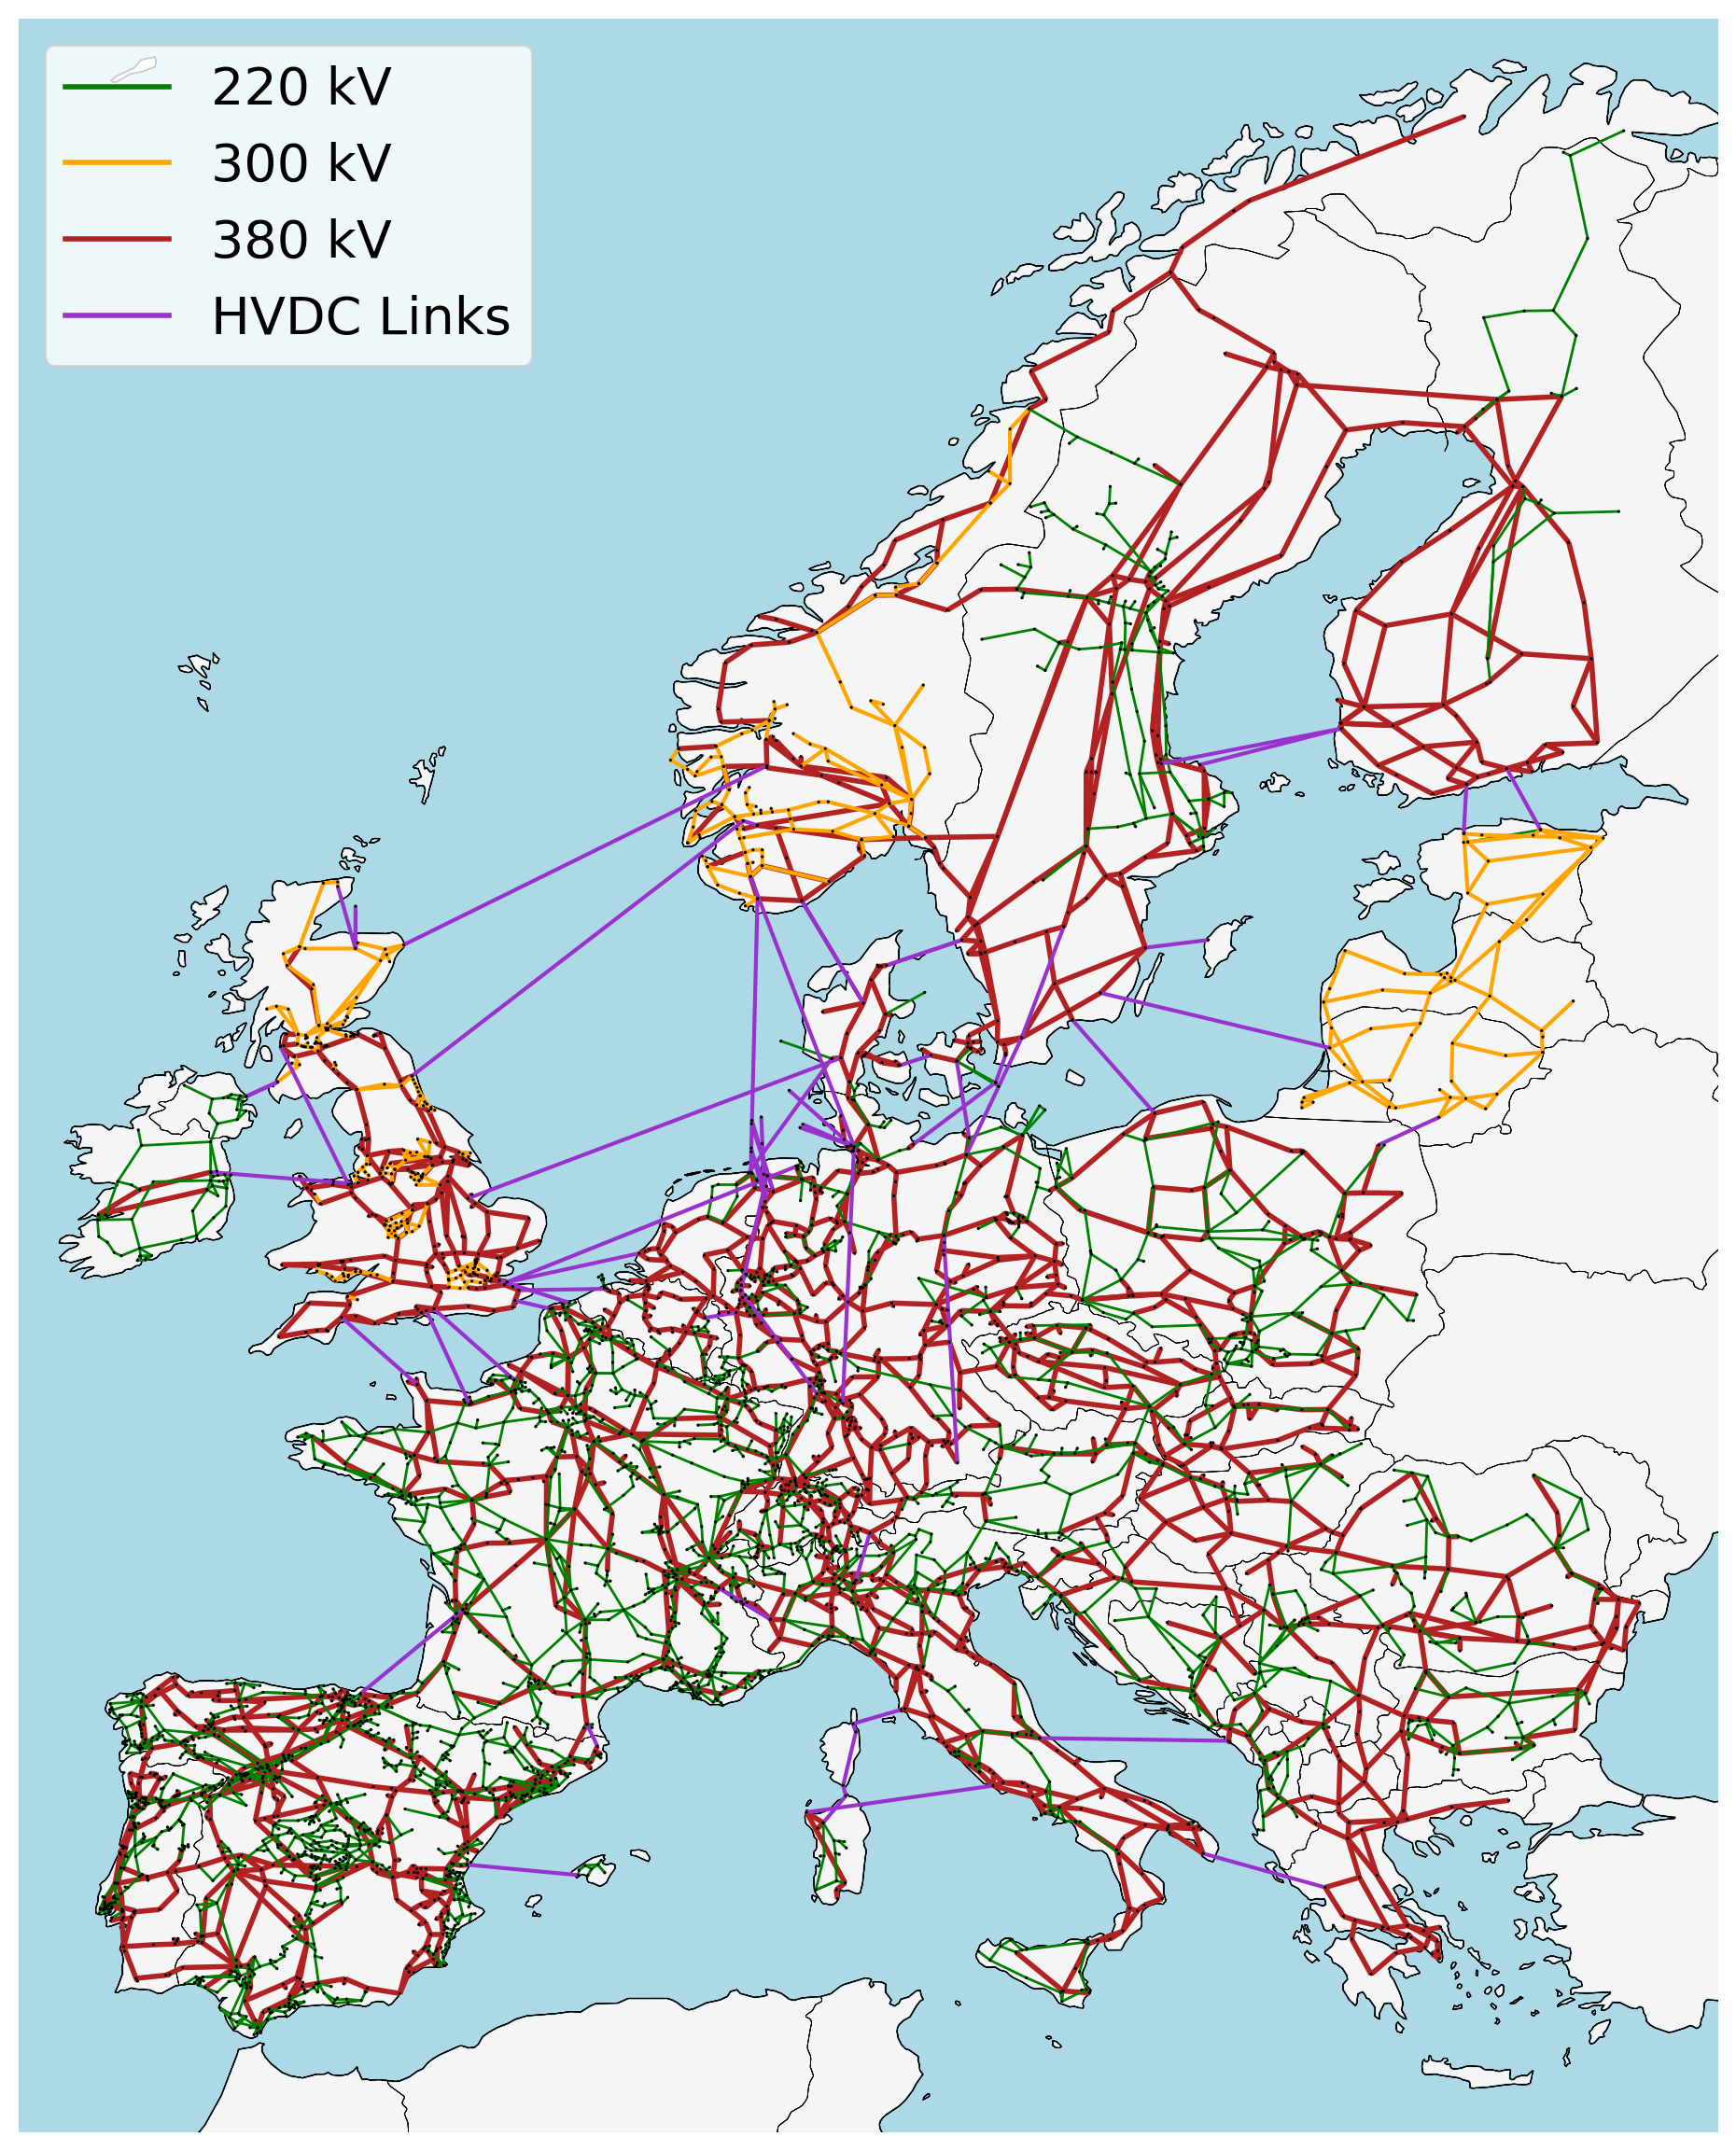
\includegraphics[width=6.5cm]{images/pypsa-eur-grid.png}

  {\footnotesize 
  \vspace{.1cm}
  Basic validation of grid model in 
  \hrefc{https://doi.org/10.1016/j.esr.2018.08.012}{Hörsch et al. (2018)}
  }
  \end{column}

  \begin{column}{8cm}
  {\footnotesize
  \begin{itemize}
    \item Grid data contains AC lines at and above 220~kV voltage level, 
    all high voltage DC lines, and substations for the full 
    \hrefc{https://www.entsoe.eu/data/map/}{ENTSO-E area}.
    \item Grid data is collected by a modified \faGithub~\hrefc{https://github.com/PyPSA/GridKit}{GridKit} extraction of the \hrefc{https://www.entsoe.eu/data/map/}{ENTSO-E Transmission System Map}. GridKit uses spatial and topological analysis to transform map objects from the ENTSO-E interactive map into a network model of the electric power system. The full grid model contains near 6760 lines and 3640 substations. 
    \item The number of nodes fed into optimization model is adjustable, what allows for spatial and topological analysis at 
    \hrefc{https://pypsa-eur.readthedocs.io/en/latest/spatial_resolution.html}{different levels}. The number of nodes can vary between 37 (the number of independent countries / synchronous areas) and several hundred (for computational tractability).\\
  \end{itemize}
  }
  
  \end{column}
  \end{columns}

  \source{Image: \href{https://github.com/PyPSA/pypsa-eur}{github.com/PyPSA/pypsa-eur}}
\end{frame}



\begin{frame}{Data sources: power plants}
 
  \begin{columns}[T]\

  \begin{column}{8cm}
    {\footnotesize 
    \begin{itemize}
      \item Existing power generation fleet data is collected with a \href{https://github.com/PyPSA/powerplantmatching}{\alert{powerplantmatching}} toolset.
      
      \item Powerplantmatching cleans, standardizes and merges the data from multiple open \hrefc{https://powerplantmatching.readthedocs.io/en/latest/basics.html}{power plant datasets} to create a combined dataset, which includes all the important information about power plants in Europe in a ready-to-use format for energy system modelling. 
      
      \item The toolset allows to update the combined data as soon as new input datasets are released.
  
      \item Powerplantmatching is an open-source project maintained by TU Berlin team. \\
      \faGithub~\hrefc{https://github.com/PyPSA/powerplantmatching}{GitHub} \\
      \faBook~\hrefc{https://powerplantmatching.readthedocs.io/en/latest/index.html}{Documentation}
    
    \end{itemize}
    }  
  \end{column}

  \begin{column}{8cm}
  \vspace{0.2cm}
  \centering
  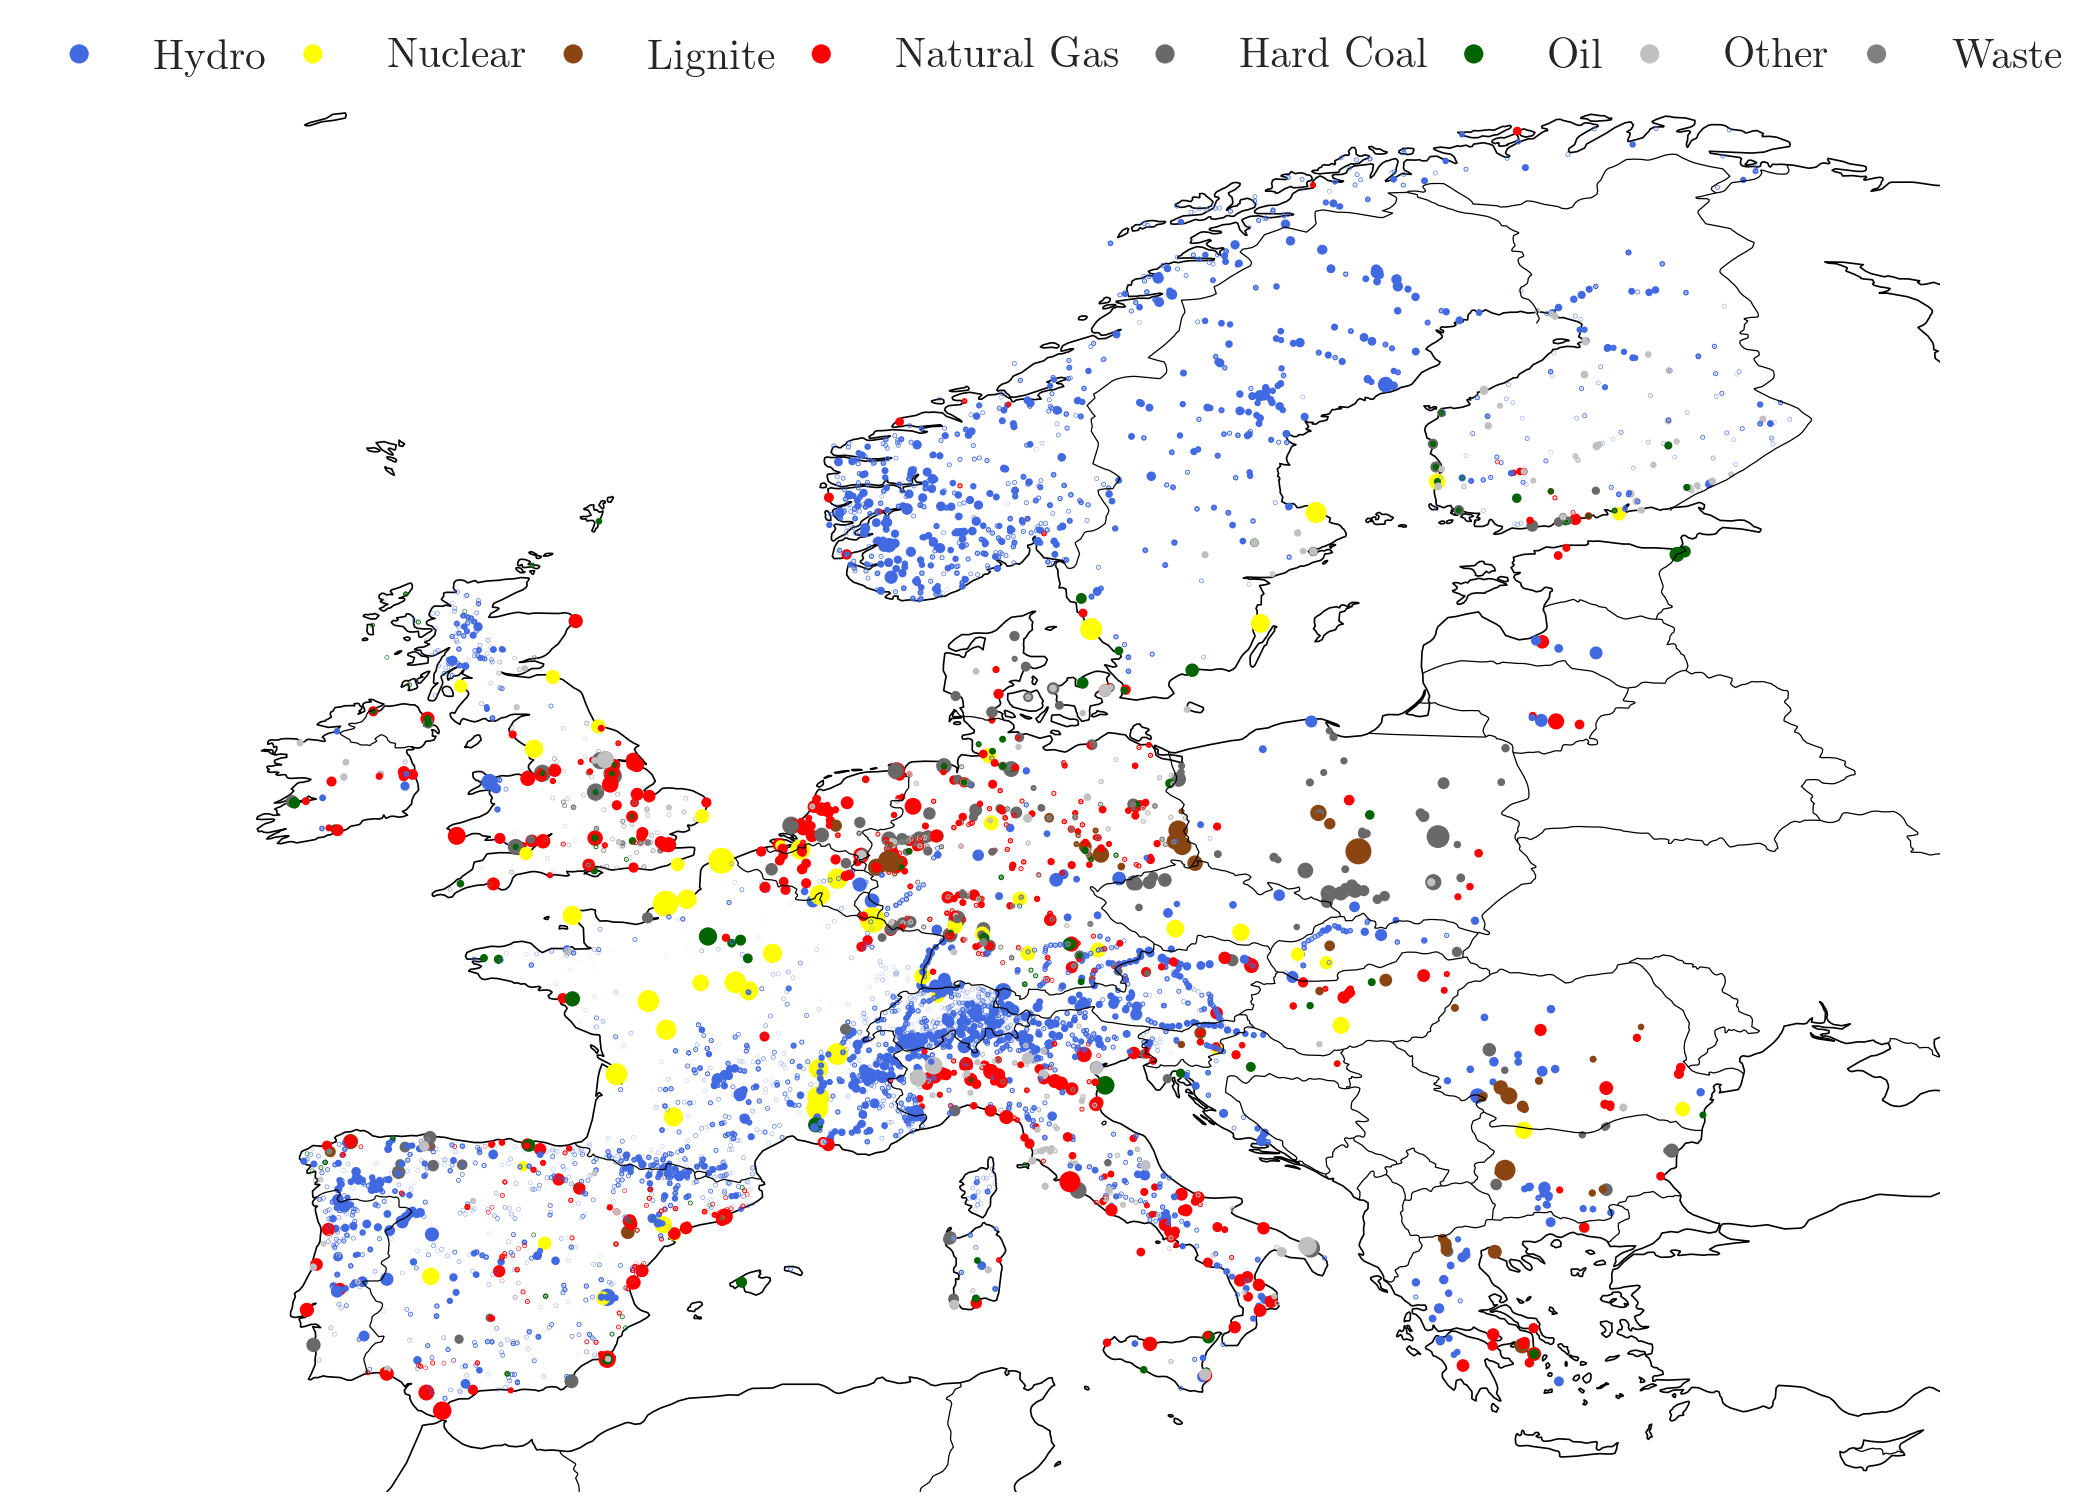
\includegraphics[width=8cm]{images/powerplantmatching.png}
  \end{column}

  \end{columns}
  \source{Image: \href{https://github.com/PyPSA/powerplantmatching}{github.com/PyPSA/powerplantmatching}}

\end{frame}



\begin{frame}{Data sources: technology cost assumptions}
 
  \begin{columns}[T]\

  \begin{column}{8cm}
    {\footnotesize 
    \begin{itemize}
      \item The database of assumptions for energy system technologies (such as capital and operational costs, efficiencies, lifetimes, etc.) is retrieved from the repository \alert{\href{https://github.com/pypsa/technology-data}{PyPSA/technology-data}}. 
      
      \item The technology-data project compiles information about energy technologies from a variety of sources. The complied dataset has standardized technology names and energy units. All values are linked to original sources.

      \item  technology-data is an open-source project maintained by TU Berlin team. \\
      \faGithub~\hrefc{https://github.com/PyPSA/technology-data}{GitHub} \\
      \faBook~\hrefc{https://technology-data.readthedocs.io/en/latest/}{Documentation}

    \end{itemize}}  
  \end{column}

  \begin{column}{7cm}
  \centering
  
\includegraphics[width=7.2cm]{images/technology-data.png}
  \vspace{0.5cm}
  {\footnotesize
  \begin{flushright}
    Cost assumptions used in this study originate from the \hrefc{https://ens.dk/en/our-services/projections-and-models/technology-data}{technology data catalogue} published by The~Danish~Energy~Agency.
  \end{flushright}
  }
  \end{column}
  \end{columns}

  \source{Image: \href{https://github.com/PyPSA/technology-data}{github.com/PyPSA/technology-data}}
\end{frame}



\begin{frame}{Data sources: renewable potentials and time series}
 
  \begin{columns}[T]
  \begin{column}{7.5cm}

  \vspace{0.5cm}
  \centering

  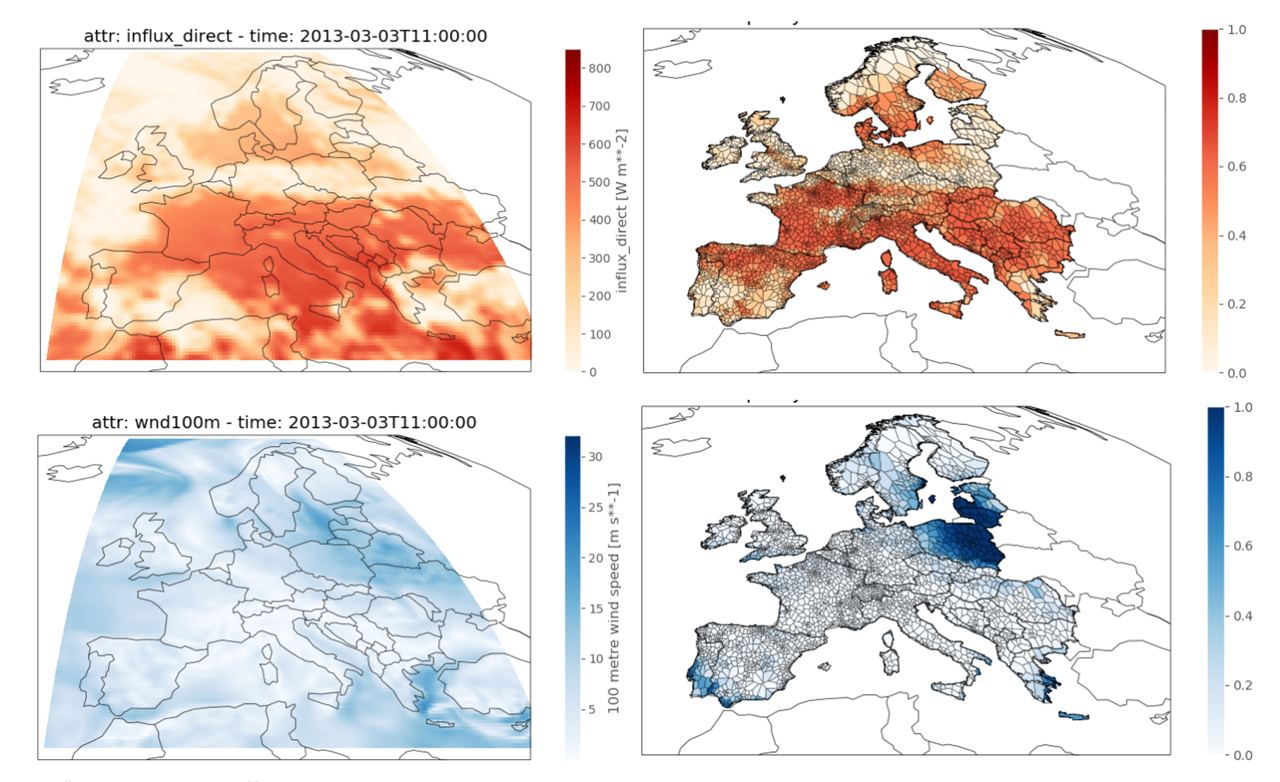
\includegraphics[width=7.8cm]{images/atlite.jpg}

  {\footnotesize 
  Converting weather data to energy system data
  }
  \end{column}

  \begin{column}{8cm}
  {\footnotesize 
  \begin{itemize}
    \item Renewable power potentials and generation profiles are processed by 
    the \href{https://github.com/PyPSA/atlite}{\alert{atlite}} package, 
    which converts terabytes of weather data (like wind speeds, solar influx) 
    into the data for energy systems modelling.
    \item With atlite, we process datasets for land cover (CORINE2018), natural protection areas (NATURA2000), and bathymetry (GEBCO2018) to conduct own geospatial land availability analysis.
    \item The standard data source for renewable time time-series estimation is ECMWF's ERA5 dataset (reanalysis weather data in ca. 30km x 30km and hourly resolution). 
    \item  atlite is also an open-source project maintained by TU~Berlin team. \\
    \faGithub~\hrefc{https://github.com/PyPSA/atlite}{GitHub} \\
    \faBook~\hrefc{https://atlite.readthedocs.io/en/latest/}{Documentation}

  \end{itemize}
  }
  \end{column}
  \end{columns}

\source{Image: \href{https://github.com/PyPSA/atlite}{atlite.readthedocs.io/}}
\end{frame}



\begin{frame}{Other background system assumptions}

\begin{itemize}
  {\footnotesize 
\item Electrical demand time-series is based on the 
\hrefc{https://open-power-system-data.org/}{OPSD project}. 
We assume the same demand profile per bidding zone for 2025 and 2030, as in the representative year 2013. 
\item We assume 2013 as the representative climate year for renewable in-feed.
\item Renewable expansion in the background electricity system is endogenous; we implement renewable generation targets by country that follow the \hrefc{https://energy.ec.europa.eu/topics/energy-strategy/national-energy-and-climate-plans-necps_en}{national energy and climate plans}. For countries w/o a 2025 target, a linear increase from renewable generation in 2020 to 2030 target is assumed. The modelled \co~emission intensity of electricity generation in European energy system matches the \hrefc{https://www.eea.europa.eu/ims/greenhouse-gas-emission-intensity-of-1}{estimated values} for 2025/2030.
\item  National policies and decommissioning plans for coal and nuclear 
power plants are based on the 
\hrefc{https://beyond-coal.eu/}{Europe Beyond Coal}, 
and \hrefc{https://world-nuclear.org/}{world-nuclear.org} projects.
\item We assume price for EU ETS allowances to be 80~\euro/tCO$_2$ for 2025.
The price for natural gas is assumed to be 35~\euro/MWh.\footnote{{\scriptsize Aligned with natural gas price assumptions in the \hrefc{https://energy.ec.europa.eu/system/files/2022-05/SWD_2022_230_1_EN_autre_document_travail_service_part1_v3.pdf}{REPowerEU Plan}
issued by the European Commission in 2022.}}
}
\vspace{0.2cm}
\end{itemize}

\end{frame}


\begin{frame}{Assumptions about technologies available for 24/7~CFE consumers}
  
  \centering
  {\footnotesize 

    \begin{tabular}{cccccccc}
      \hline
      \hline
      Year & Technology & CAPEX & FOM & VOM & Efficiency & lifetime \\
       &  & (overnight cost)  &  (\%/year) &  (€/MWh) & (per unit) & (years) \\
      \hline
      \hline
      2025 & utility solar PV & 612 €/kW & 1.7 & 0.01 & - & 37.5 \\
      \hline
      2025 & onshore wind & 1077 €/kW & 1.2 & 0.015 & - & 28.5 \\
      \hline
      2025 & battery storage & 187 €/kWh & 0 & - & - & 22.5 \\
      \hline
      2025  & battery inverter & 215 €/kW & 0.3 & - & 0.96  & 10.0 \\
      \hline
      2025 & hydrogen storage\footnote{{\scriptsize Underground hydrogen storage in salt cavern}} 
                  & 2.5 €/kWh & 0 & - & - & 100.0 \\
      \hline
      2025 & electrolysis & 550 €/kW & 2.0 & - & 0.67 & 27.5  \\
      \hline
      2025 & fuel cell & 1200 €/kW & 5.0 & - & 0.50 & 10.0 \\
      \hline
      \hline
      % 2030 & utility solar PV & 492 €/kW & 2.0 & 0.01 & - & 40.0 \\
      % \hline
      % 2030 & onshore wind & 1035 €/kW & 1.2 & 0.015 & - & 30 \\
      % \hline
      % 2030 & battery storage & 142 €/kWh & 0 & - & - & 25 \\
      % \hline
      % 2030  & battery inverter & 160 €/kW & 0.3 & - & 0.96  & 10.0 \\
      % \hline
      % 2030 & hydrogen storage  & 2.0 €/kWh & 0 & - & - & 100.0 \\
      % \hline
      % 2030 & electrolysis & 450 €/kW & 2.0 & - & 0.68 & 30  \\
      % \hline
      % 2030 & fuel cell & 1100 €/kW & 5.0 & - & 0.50 & 10.0 \\
      % \hline
      % \hline
      \end{tabular}
  
    Data is originally retrieved from the \hrefc{https://ens.dk/en/our-services/projections-and-models/technology-data}{DEA's catalogue for energy technologies}
      \vspace{0.2cm}
  }
\end{frame}

%----------------------------------------
%----------------------------------------

\section{Annex C: Supplementary graphics}


%---------------------------------------- Carbon Heat Maps
%----------------------------------------


\begin{frame}{Hourly CFE score of supply from grid -- DE 2025}
  \label{CFEheatmaps}
  \vspace{.5cm}
  \includegraphics[height=5.5cm]{../results/1H-IEDKDEFIPT-spatial/plots/2025/EU/p1/cfe100/heatmaps/0_GridCFE_DE1 0.pdf}
\end{frame}

\begin{frame}{Hourly CFE score of supply from grid -- DK 2025}
  \vspace{.5cm}
  \includegraphics[height=5.5cm]{../results/1H-IEDKDEFIPT-spatial/plots/2025/EU/p1/cfe100/heatmaps/0_GridCFE_DK1 0.pdf}
\end{frame}

\begin{frame}{Hourly CFE score of supply from grid -- IE 2025}
  \vspace{.5cm}
  \includegraphics[height=5.5cm]{../results/1H-IEDKDEFIPT-spatial/plots/2025/EU/p1/cfe100/heatmaps/0_GridCFE_IE5 0.pdf}
\end{frame}

\begin{frame}{Hourly CFE score of supply from grid -- FI 2025}
  \vspace{.5cm}
  \includegraphics[height=5.5cm]{../results/1H-IEDKDEFIPT-spatial/plots/2025/EU/p1/cfe100/heatmaps/0_GridCFE_FI2 0.pdf}
\end{frame}


%---------------------------------------- Isolated values story
%----------------------------------------

\begin{frame}{24/7~CFE costs as a function of load flexibility:\\
  isolated spatial load shifting}
  \label{isolated_spatial_cfe100_p1}

  {\footnotesize
  
  Isolating values of spatial and temporal load management for a scenario with {\bf CFE score of 100\% and technology palette~1}. 
  The plots below show the average costs (per MWh of consumption) {\bf (left)} and the net annual costs (per annum) for achieving 24/7 policy in all locations {\bf (right)} with {\bf spatial} load shifting.

  \begin{columns}[T]
  \begin{column}{8cm}
  \centering
  \includegraphics[width=8cm]{../results/1H-IEDKDEFIPT-spatial/plots/2025/EU/p1/cfe100/ci_costandrev.pdf}
  \end{column}

  \begin{column}{7cm}
    \includegraphics[width=7cm]{../results/1H-IEDKDEFIPT-spatial/plots/2025/EU/p1/cfe100/ci_abs_costs.pdf}
  \end{column}
  \end{columns}
  }
  \source{24/7 CFE 100\% -- palette~1 tech -- spatial shifts}
\end{frame}


\begin{frame}{24/7~CFE costs as a function of load flexibility:\\
  isolated temporal load shifting}
  \label{isolated_temporal_cfe100_p1}

  {\footnotesize
  
  Isolating values of spatial and temporal load management for a scenario with {\bf CFE score of 100\% and technology palette~1}. 
  The plots below show the average costs (per MWh of consumption) {\bf (left)} and the net annual costs (per annum) for achieving 24/7 policy in all locations {\bf (right)} with {\bf temporal} load shifting.

  \begin{columns}[T]
  \begin{column}{8cm}
  \centering
  \includegraphics[width=8cm]{../results/1H-IEDKDEFIPT-temporal/plots/2025/EU/p1/cfe100/ci_costandrev.pdf}
  \end{column}

  \begin{column}{7cm}
    \includegraphics[width=7cm]{../results/1H-IEDKDEFIPT-temporal/plots/2025/EU/p1/cfe100/ci_abs_costs.pdf}
  \end{column}
  \end{columns}
  }
  \source{24/7 CFE 100\% -- palette~1 tech -- temporal shifts}
\end{frame}


%---------------------------------------- Curtailment
%----------------------------------------

\begin{frame}{Reduction of renewable energy curtailment}
  \label{curtailment}
  
    {\footnotesize
  The plots below show the absolute amount of energy curtailment [GWh] from the portfolio of CFE generators procured by a data center operator as a function of load flexibility. The results are displayed per share of flexible loads $f = \{0\%, 10\%, 20\%, 40\%\}$.
  \\
  {\bf Left panel}: technology palette 1 (no LDES); {\bf right panel}: technology palette 2 (with LDES)
    
    \vspace{0.3cm} 
    \begin{columns}
      \begin{column}{7cm}
      \includegraphics[width=7cm]{../results/1H-IEDKDEFIPT-allflex/plots/2025/EU/p1/cfe100/ci_curtailment.pdf}
      \end{column}
      
      \begin{column}{7cm}
      \includegraphics[width=7cm]{../results/1H-IEDKDEFIPT-allflex/plots/2025/EU/p2/cfe100/ci_curtailment.pdf}
      \end{column}
    \end{columns}
  
    \source{24/7 CFE 100\% -- palettes 1 and 2 -- spatial \& temporal shifts}
    }
    
  \end{frame}

%---------------------------------------- Nodal balances
%----------------------------------------

\begin{frame}{Data center CFE supply and demand}
  \label{nb1-40}

  {\footnotesize
  
  \begin{columns}[T]
    \begin{column}{3.5cm}
      \vspace{0.3cm}
      The plot on the right shows the {\bf nodal energy balance} [MW*h/h], i.e., the (cost-optimal) matching of data center consumption with carbon-free energy supply.

      \vspace{0.2cm}
      Data center in Ireland. \\
      The first week of March. \\
      40\% of flexible workloads.\\
      100\% CFE score.\\
    \end{column}
  
    \begin{column}{11cm}
      \includegraphics[width=11cm]{../results/1H-IEDKDEFIPT-allflex/plots/2025/EU/p1/cfe100/03.01-03.08/40_balance_ireland.pdf}
    \end{column}
    \end{columns}
    } 

  \source{DC in IE zone -- 24/7 CFE 100\% -- palette~1 tech -- spatial \& temporal shifts -- 40\% flexible workloads}
\end{frame}



\begin{frame}{Data center CFE supply and demand}
  \label{nb1-10}

  {\footnotesize
  
  \begin{columns}[T]
    \begin{column}{3.5cm}
      \vspace{0.3cm}
      The plot on the right shows the {\bf nodal energy balance} [MW*h/h], i.e., the (cost-optimal) matching of data center consumption with carbon-free energy supply.

      \vspace{0.2cm}
      Data center in Ireland. \\
      The first week of March. \\
      10\% of flexible workloads.\\
      100\% CFE score.\\
    \end{column}
  
    \begin{column}{11cm}
      \includegraphics[width=11cm]{../results/1H-IEDKDEFIPT-allflex/plots/2025/EU/p1/cfe100/03.01-03.08/10_balance_ireland.pdf}
    \end{column}
    \end{columns}
    } 

  \source{DC in IE zone -- 24/7 CFE 100\% -- palette~1 tech -- spatial \& temporal shifts -- 10\% flexible workloads}
\end{frame}


\begin{frame}{Data center CFE supply and demand}
  \label{nb2-40}

  {\footnotesize
  
  \begin{columns}[T]
    \begin{column}{3.5cm}
      \vspace{0.3cm}
      The plot on the right shows the {\bf nodal energy balance} [MW*h/h], i.e., the (cost-optimal) matching of data center consumption with carbon-free energy supply.

      \vspace{0.2cm}
      Data center in Denmark. \\
      The first week of March. \\
      40\% of flexible workloads.\\
      100\% CFE score.\\
    \end{column}
  
    \begin{column}{11cm}
      \includegraphics[width=11cm]{../results/1H-IEDKDEFIPT-allflex/plots/2025/EU/p1/cfe100/03.01-03.08/40_balance_denmark.pdf}
    \end{column}
    \end{columns}
    } 

  \source{DC in DK1 zone -- 24/7 CFE 100\% -- palette~1 tech -- spatial \& temporal shifts -- 40\% flexible workloads}
\end{frame}


\begin{frame}{Data center CFE supply and demand}
  \label{nb2-10}

  {\footnotesize
  
  \begin{columns}[T]
    \begin{column}{3.5cm}
      \vspace{0.3cm}
      The plot on the right shows the {\bf nodal energy balance} [MW*h/h], i.e., the (cost-optimal) matching of data center consumption with carbon-free energy supply.

      \vspace{0.2cm}
      Data center in Denmark. \\
      The first week of March. \\
      10\% of flexible workloads.\\
      100\% CFE score.\\
    \end{column}
  
    \begin{column}{11cm}
      \includegraphics[width=11cm]{../results/1H-IEDKDEFIPT-allflex/plots/2025/EU/p1/cfe100/03.01-03.08/10_balance_denmark.pdf}
    \end{column}
    \end{columns}
    } 

  \source{DC in DK1 zone -- 24/7 CFE 100\% -- palette~1 tech -- spatial \& temporal shifts -- 10\% flexible workloads}
\end{frame}


\begin{frame}{Data center CFE supply and demand}
  \label{nb3}

  {\footnotesize
  
  \begin{columns}[T]
    \begin{column}{3.5cm}
      \vspace{0.3cm}
      The plot on the right shows the {\bf nodal energy balance} [MW*h/h], i.e., the (cost-optimal) matching of data center consumption with carbon-free energy supply.

      \vspace{0.2cm}
      Data center in Germany. \\
      The first week of May. \\
      40\% of flexible workloads.\\
      100\% CFE score.\\
    \end{column}
  
    \begin{column}{11cm}
      \includegraphics[width=11cm]{../results/1H-IEDKDEFIPT-allflex/plots/2025/EU/p1/cfe100/05.01-05.08/40_balance_germany.pdf}
    \end{column}
    \end{columns}
    } 

  \source{DC in DE zone -- 24/7 CFE 100\% -- palette~1 tech -- spatial \& temporal shifts -- 40\% flexible workloads}
\end{frame}

%---------------------------------------- supplementary for temporal story

\begin{frame}{Data center CFE supply and demand}
  \label{nbtemp-40-PT}

  {\footnotesize
  
  \begin{columns}[T]
    \begin{column}{3.5cm}
      \vspace{0.3cm}
      The plot on the right shows the {\bf nodal energy balance} [MW*h/h], i.e., the (cost-optimal) matching of data center consumption with carbon-free energy supply.

      \vspace{0.2cm}
      Data center in Portugal. \\
      The first week of May. \\
      40\% of flexible workloads.\\
      98\% CFE score.\\

    \end{column}
  
    \begin{column}{11cm}
      \includegraphics[width=11cm]{../results/1H-IEDKDEFIPT-allflex/plots/2025/EU/p1/cfe98/05.01-05.08/40_balance_portugal.pdf}
    \end{column}
    \end{columns}
    } 

  \source{DC in PT zone -- 24/7 CFE 98\% -- palette~1 tech -- spatial \& temporal shifts -- 40\% flexible workloads}
\end{frame}


\begin{frame}{Data center CFE supply and demand}
  \label{nbtemp-40-IE}

  {\footnotesize
  
  \begin{columns}[T]
    \begin{column}{3.5cm}
      \vspace{0.3cm}
      The plot on the right shows the {\bf nodal energy balance} [MW*h/h], i.e., the (cost-optimal) matching of data center consumption with carbon-free energy supply.

      \vspace{0.2cm}
      Data center in Ireland. \\
      The first week of December. \\
      40\% of flexible workloads.\\
      98\% CFE score.\\

    \end{column}
  
    \begin{column}{11cm}
      \includegraphics[width=11cm]{../results/1H-IEDKDEFIPT-allflex/plots/2025/EU/p1/cfe98/12.01-12.08/40_balance_ireland.pdf}
    \end{column}
    \end{columns}
    } 

  \source{DC in IE zone -- 24/7 CFE 98\% -- palette~1 tech -- spatial \& temporal shifts -- 40\% flexible workloads}
\end{frame}


%---------------------------------------- supplementary for LDES


\begin{frame}{Data center CFE supply and demand}
  \label{nbp2-IE-40}

  {\footnotesize
  
  \begin{columns}[T]
    \begin{column}{3.5cm}
      \vspace{0.3cm}
      The plot on the right shows the {\bf nodal energy balance} [MW*h/h], i.e., the (cost-optimal) matching of data center consumption with carbon-free energy supply.

      \vspace{0.2cm}
      Data center in Ireland. \\
      The first week of March. \\
      40\% of flexible workloads.\\
      100\% CFE score.\\
      + LDES (palette~2). \\

    \end{column}
  
    \begin{column}{11cm}
      \includegraphics[width=11cm]{../results/1H-IEDKDEFIPT-allflex/plots/2025/EU/p2/cfe100/03.01-03.08/40_balance_ireland.pdf}
    \end{column}
    \end{columns}
    } 

  \source{DC in IE zone -- 24/7 CFE 100\% -- palette~2 tech -- spatial \& temporal shifts -- 40\% flexible workloads}
\end{frame}


\begin{frame}{Data center CFE supply and demand}
  \label{nbp2-IE-0}

  {\footnotesize
  
  \begin{columns}[T]
    \begin{column}{3.5cm}
      \vspace{0.3cm}
      The plot on the right shows the {\bf nodal energy balance} [MW*h/h], i.e., the (cost-optimal) matching of data center consumption with carbon-free energy supply.

      \vspace{0.2cm}
      Data center in Ireland. \\
      The first week of March. \\
      0\% of flexible workloads.\\
      100\% CFE score.\\
      + LDES (palette~2).

    \end{column}
  
    \begin{column}{11cm}
      \includegraphics[width=11cm]{../results/1H-IEDKDEFIPT-allflex/plots/2025/EU/p2/cfe100/03.01-03.08/0_balance_ireland.pdf}
    \end{column}
    \end{columns}
    } 

  \source{DC in IE zone -- 24/7 CFE 100\% -- palette~2 tech -- spatial \& temporal shifts -- 0\% flexible workloads}
\end{frame}



\begin{frame}{Data center CFE supply and demand}
  \label{nbp2-DK-40}

  {\footnotesize
  
  \begin{columns}[T]
    \begin{column}{3.5cm}
      \vspace{0.3cm}
      The plot on the right shows the {\bf nodal energy balance} [MW*h/h], i.e., the (cost-optimal) matching of data center consumption with carbon-free energy supply.

      \vspace{0.2cm}
      Data center in Denmark. \\
      The first week of March. \\
      40\% of flexible workloads.\\
      100\% CFE score.\\
      + LDES (palette~2). \\

    \end{column}
  
    \begin{column}{11cm}
      \includegraphics[width=11cm]{../results/1H-IEDKDEFIPT-allflex/plots/2025/EU/p2/cfe100/03.01-03.08/40_balance_denmark.pdf}
    \end{column}
    \end{columns}
    } 

  \source{DC in DK zone -- 24/7 CFE 100\% -- palette~2 tech -- spatial \& temporal shifts -- 40\% flexible workloads}
\end{frame}



\begin{frame}{Data center CFE supply and demand}
  \label{nbp2-DK-0}

  {\footnotesize
  
  \begin{columns}[T]
    \begin{column}{3.5cm}
      \vspace{0.3cm}
      The plot on the right shows the {\bf nodal energy balance} [MW*h/h], i.e., the (cost-optimal) matching of data center consumption with carbon-free energy supply.

      \vspace{0.2cm}
      Data center in Denmark. \\
      The first week of March. \\
      0\% of flexible workloads.\\
      100\% CFE score.\\
      + LDES (palette~2). \\

    \end{column}
  
    \begin{column}{11cm}
      \includegraphics[width=11cm]{../results/1H-IEDKDEFIPT-allflex/plots/2025/EU/p2/cfe100/03.01-03.08/0_balance_denmark.pdf}
    \end{column}
    \end{columns}
    } 

  \source{DC in DK zone -- 24/7 CFE 100\% -- palette~2 tech -- spatial \& temporal shifts -- 0\% flexible workloads}
\end{frame}


\end{document}
%----------------------------------------
%----------------------------------------